\documentclass[10pt]{amsart}
\usepackage[a4paper,margin=23mm]{geometry}
\usepackage{amsmath,amssymb,amsthm,mathtools,hyperref,graphicx,xspace,letltxmacro,xpatch}
\usepackage[english]{babel}
\newtheorem{theo}{Theorem}[section]
\newtheorem{lemm}[theo]{Lemma}\newtheorem{prop}[theo]{Proposition}\newtheorem{coro}[theo]{Corollary}\newtheorem{conj}[theo]{Conjecture}
\theoremstyle{definition}\newtheorem{defi}[theo]{Definition}\newtheorem{rema}[theo]{Remark}\newtheorem{exam}[theo]{Example}\newtheorem{exem}[theo]{Example}\newtheorem{nota}[theo]{Notation}
\newcommand{\ie}{i.e.}\newcommand{\eg}{e.g.}\newcommand{\resp}{resp.}\newcommand{\skpt}{\par\smallskip\noindent}
\emergencystretch=3em\pagestyle{plain}
%~Mouliné par MaN_auto v.0.23.0 2020-05-25 16:49:39
%
%\makeatletter
%%\def\@altabstractlanguage{}
%\makeatother


\usepackage{tikz}
\usepackage{tkz-tab}
\usepackage{array}
%\usepackage[normalem]{ulem}
%\usepackage{multirow}
%\usepackage{amscd}
\usepackage{mathtools}

\DeclarePairedDelimiter{\vect}{\langle}{\rangle}

\let\oldtilde\tilde
\renewcommand*{\tilde}[1]{\mathchoice{\widetilde{#1}}{\widetilde{#1}}{\oldtilde{#1}}{\oldtilde{#1}}}
\let\oldhat\hat
\renewcommand*{\hat}[1]{\mathchoice{\widehat{#1}}{\widehat{#1}}{\oldhat{#1}}{\oldhat{#1}}}

\makeatletter
\let\save@mathaccent\mathaccent
\newcommand*\if@single[3]{%
  \setbox0\hbox{${\mathaccent"0362{#1}}^H$}%
  \setbox2\hbox{${\mathaccent"0362{\kern0pt#1}}^H$}%
  \ifdim\ht0=\ht2 #3\else #2\fi
  }
%The bar will be moved to the right by a half of \macc@kerna, which is computed by amsmath:
\newcommand*\rel@kern[1]{\kern#1\dimexpr\macc@kerna}
%If there's a superscript following the bar, then no negative kern may follow the bar;
%an additional {} makes sure that the superscript is high enough in this case:
\newcommand*\widebar[1]{\@ifnextchar^{{\wide@bar{#1}{0}}}{\wide@bar{#1}{1}}}
%Use a separate algorithm for single symbols:
\newcommand*\wide@bar[2]{\if@single{#1}{\wide@bar@{#1}{#2}{1}}{\wide@bar@{#1}{#2}{2}}}
\newcommand*\wide@bar@[3]{%
  \begingroup
  \def\mathaccent##1##2{%
%Enable nesting of accents:
    \let\mathaccent\save@mathaccent
%If there's more than a single symbol, use the first character instead (see below):
    \if#32 \let\macc@nucleus\first@char \fi
%Determine the italic correction:
    \setbox\z@\hbox{$\macc@style{\macc@nucleus}_{}$}%
    \setbox\tw@\hbox{$\macc@style{\macc@nucleus}{}_{}$}%
    \dimen@\wd\tw@
    \advance\dimen@-\wd\z@
%Now \dimen@ is the italic correction of the symbol.
    \divide\dimen@ 3
    \@tempdima\wd\tw@
    \advance\@tempdima-\scriptspace
%Now \@tempdima is the width of the symbol.
    \divide\@tempdima 10
    \advance\dimen@-\@tempdima
%Now \dimen@ = (italic correction / 3) - (Breite / 10)
    \ifdim\dimen@>\z@ \dimen@0pt\fi
%The bar will be shortened in the case \dimen@<0 !
    \rel@kern{0.6}\kern-\dimen@
    \if#31
      \overline{\rel@kern{-0.6}\kern\dimen@\macc@nucleus\rel@kern{0.4}\kern\dimen@}%
      \advance\dimen@0.4\dimexpr\macc@kerna
%Place the combined final kern (-\dimen@) if it is >0 or if a superscript follows:
      \let\final@kern#2%
      \ifdim\dimen@<\z@ \let\final@kern1\fi
      \if\final@kern1 \kern-\dimen@\fi
    \else
      \overline{\rel@kern{-0.6}\kern\dimen@#1}%
    \fi
  }%
  \macc@depth\@ne
  \let\math@bgroup\@empty \let\math@egroup\macc@set@skewchar
  \mathsurround\z@ \frozen@everymath{\mathgroup\macc@group\relax}%
  \macc@set@skewchar\relax
  \let\mathaccentV\macc@nested@a
%The following initialises \macc@kerna and calls \mathaccent:
  \if#31
    \macc@nested@a\relax111{#1}%
  \else
%If the argument consists of more than one symbol, and if the first token is
%a letter, use that letter for the computations:
    \def\gobble@till@marker##1\endmarker{}%
    \futurelet\first@char\gobble@till@marker#1\endmarker
    \ifcat\noexpand\first@char A\else
      \def\first@char{}%
    \fi
    \macc@nested@a\relax111{\first@char}%
  \fi
  \endgroup
}
\makeatother
\let\oldbar\bar
\renewcommand*{\bar}[1]{\mathchoice{\widebar{#1}}{\widebar{#1}}{\oldbar{#1}}{\oldbar{#1}}}

%%%%%%%%%%%%%%


\newcounter{a}
\setcounter{a}{0}
\newcommand{\Cond}{Cond.}
\newenvironment{cond}{\refstepcounter{a}{\upshape\emph{Cond.~\thea}}\pointir}{}
\newenvironment{condd}{{\upshape\emph{Cond~\thea*}\pointir}}{}
\newenvironment{conddd}[1]{{\upshape\emph{Cond~\ref{#1}}\pointir}}{}

%\theoremstyle{remark}
%\newtheorem{cond}{Cond.}
%\newtheorem{condd}{Cond.}
%\renewcommand*{\thecondd}{\thecond*}


\newcommand{\tT}{\tilde T}

\newcommand{\encadre}[1]{\begin{tabular}{|c|} \hline #1 \\ \hline\end{tabular}}
% Ça marchait pas trop mal, mais je trouve que ma version est un peu mieux
\newcommand{\myencadre}[2][5.1cm]{\vspace{0.15cm}\fbox{\parbox{#1}{#2}}\vspace{0.15cm}}
 
\newcommand{\app}[5]{\begin{array}{rccl} #1:&#2&\longrightarrow &#3\\ &#4&\longmapsto &#5\end{array}}
%\newcommand{\rv}[1]{\mathbf{#1}}

%% Commande ci dessous désactivée en raison des problèmes d'alignement causées dans les formules :
%%remplacement en manuel
%%\newcommand{\prob}[1]{\mathbb{P}\left(#1\right)}

%%COMMANDES OK
\newcommand{\pw}[1]{\mathbb{P}_W\left(#1\right)}
\newcommand{\eqd}{\stackrel{(d)}{=}}
\newcommand{\ind}[1]{1_{#1}}
\newcommand{\diff}[1]{\mathrm{d} #1}
%%\DeclareMathOperator{\diff}{d}
\newcommand{\borel}[1]{\mathcal{B}\left(#1 \right)}
\newcommand{\triang}[2]{\mathcal{T}_{#1} \left(#2 \right)}
\newcommand{\triangE}[1]{\mathcal{T}_{#1}}



%\newcommand{\id}{\mathrm{id}}%%mathop
\DeclareMathOperator{\id}{id}

%%math caract%%%%%%%%%%%%%%%%
\newcommand{\NN}{\mathbb{N}}
\newcommand{\ZZ}{\mathbb{Z}}
\newcommand{\Z}{\mathbb{Z}}
\newcommand{\Ze}{\mathbb{Z}_{\mathrm{e}^2}}
\newcommand{\RR}{\mathbb{R}}
\newcommand{\Pbb}{\mathbb{P}}

\newcommand{\ber}{\mathcal{B}}
\renewcommand{\L}{\mathcal{L}}

%%Mathop%%%%%%%%%%%%%%%%%%%%%%%%%%%%

%%\newcommand{\vu}{{\bf \textup{u}}}
\DeclareMathOperator{\vu}{u}
%%\newcommand{\vv}{{\bf \textup{v}}}
\DeclareMathOperator{\vv}{v}

\newcommand{\Fh}{M_{-\vv}}
\newcommand{\Bh}{M_{\vu}}

%%\newcommand{\sym}{\text{sym}}
\DeclareMathOperator{\sym}{sym}


%\newcommand{\M}{\mathcal{M}}

%\newcommand{\ppm}{\Pi_p}

\newcommand{\haut}[1]{$\begin{array}{c}(#1)\\ \;\end{array}$}
\newcommand{\espace}{\rule{0pt}{6ex}}
\newcommand{\test}{\vspace{0.15cm}\rule{0pt}{5ex}\vspace{0.15cm}}

%\renewcommand{\thefootnote}{\alph{footnote}}

\newcommand{\isdef}{\triangleq}


%%%%%%%%%%%%%%%%%%%%%%%%%%%%%%%%%%
\definecolor{grey}{rgb}{0.5,0.5,0.5}

\usetikzlibrary{arrows}
\usetikzlibrary{decorations.markings}
\tikzset{->-/.style={decoration={ markings, mark=at position.7 with {\arrow[scale=2]{>}}},postaction={decorate}}}
\tikzset{>>/.style={decoration={ markings, mark=at position.7 with {\arrow[scale=5]{>}}},postaction={decorate}}}
\tikzset{>>>/.style={decoration={ markings, mark=at position 1 with {\arrow[scale=5]{>}}},postaction={decorate}}}

%%%%%%%%%%%%%%%%%%%%%%%%%%%%%%%%%%%%%%%%%%

\graphicspath{{./figures/}}

\newcommand*{\mk}{\mkern -1mu}
\newcommand*{\Mk}{\mkern -2mu}
\newcommand*{\mK}{\mkern 1mu}
\newcommand*{\MK}{\mkern 2mu}

\hypersetup{urlcolor=purple, linkcolor=blue, citecolor=red}

\newcommand*{\romanenumi}{\renewcommand*{\theenumi}{\roman{enumi}}}
\newcommand*{\Romanenumi}{\renewcommand*{\theenumi}{\Roman{enumi}}}
\newcommand*{\alphenumi}{\renewcommand*{\theenumi}{\alph{enumi}}}
\newcommand*{\Alphenumi}{\renewcommand*{\theenumi}{\Alph{enumi}}}
\let\oldforall\forall
\renewcommand*{\forall}{\mathrel{\oldforall}}
%%%%%%%%%%%%%%%%%%%%%%%%%%%%%%%%%%%%%%%%%%%%%%

\providecommand{\pointir}{.\ }

\newtheorem{definition}[theo]{Definition}
\newtheorem{lemma}[theo]{Lemma}
\newtheorem{proposition}[theo]{Proposition}
\newtheorem{corollary}[theo]{Corollary}
\newtheorem{theorem}[theo]{Theorem}
\newtheorem{remark}[theo]{Remark}
\newenvironment{proofc}[1][\proofname]{\begin{proof}[{#1}]}{\end{proof}}
\title{Dimensions of multidirectionally reversible memory-two probabilistic cellular automata}
\author{Casse, Jérôme, Marcovici, Irène}
\date{doi:10.5802/ahl.39; CC BY 4.0}
\begin{document}
\maketitle
\noindent\textit{Editorial note.} Complete original mathematical body and author bibliography retained. Original embedded Forms and both raster figures with soft masks recovered. Local class wrapper only; raster resolution matches native printed scale.\par\medskip
\noindent\textit{Allowed standard prerequisites (editorial).}\begin{itemize}
\item Standard functional analysis, measure theory and the author-cited classical theorems. Standard prior results stay cited; complete source-local proofs and definitions retained.
\end{itemize}\medskip

\section{Introduction}

Probabilistic cellular automata (PCA) are a class of random discrete dynamical systems. They can be seen both as the synchronous counterparts of finite-range interacting particle systems, and as a generalization of deterministic cellular automata: time is discrete and at each time step, all the cells are updated independently in a random fashion, according to a distribution depending only on the states of a finite number of their neighbours.

In this article, we focus on a family of one-dimensional probabilistic cellular automata with \emph{memory two} (or \emph{order two}): the value of a given cell at time $t+1$ is drawn according to a distribution which is a function of the states of its two nearest neighbours at time $t$, and of its own state at time $t-1$. The space-time diagrams describing the evolution of the states can thus be represented on a two-dimensional grid.

We study the invariant measures of these PCA with memory two. In particular, we give necessary and sufficient conditions for which the invariant measure has a product form or a Markovian form, and we prove an ergodicity result holding in that context. We also show that when the parameters of the PCA satisfy some conditions, the stationary space-time diagram presents some multidirectional (quasi-)reversibility property: the random field has the same distribution as if we had iterated a PCA with memory two in another direction (the same PCA in the reversible case, or another PCA in the quasi-reversible case). This can be seen has a probabilistic extension of the notion of \emph{expansivity} for deterministic CA. For expansive CA, one can indeed reconstruct the whole space-time diagram from the knowledge of only one column. In the context of PCA with memory two, the criteria of quasi-reversibility that we obtain are reminiscent of the notion of \emph{permutivity} for deterministic CA.\linebreak Stationary space-time diagrams of PCA are known to be Gibbs random fields \cite{GKLM,LMS}. The family of PCA that we will describe thus provide examples of Gibbs fields with i.i.d. lines in many directions and nice combinatorial and geometric properties.

The first theoretical results on PCA and their invariant measures go back to the seventies~\cite{belyaev,kozlov,vasilyev}, and were then gathered in a survey which is still today a reference book~\cite{dobrushin}. In particular, it contains a detailed study of binary PCA of memory one with only two neighbours, including a presentation of the necessary and sufficient conditions that the four parameters defining the PCA must satisfy in order to have an invariant measure with a product form or a Markovian form. Some extensions and alternative proofs were proposed by Mairesse and Marcovici in a later article~\cite{mm_ihp}, together with a study of some properties of the random fields given by stationary space-time diagrams of PCA having a product form invariant measure (see also the survey on PCA of the same authors~\cite{mm_tcs}). The novelty was to highlight that these space-time diagrams are i.i.d. along many directions, and present a directional reversibility: they can also be seen as being obtained by iterating some PCA in another direction. Soon after, Casse and Marckert have proposed an in-depth study of the Markovian case~\cite{Casse16,CM15}. Motivated by the study of the $8$-vertex model, Casse was then led to introduce a class of one-dimensional PCA with memory two, called \emph{triangular PCA}~\cite{Casse17}.

In the present article, we propose a comprehensive study of PCA with memory two having an invariant measure with a product form, and we show that their stationary space-time diagrams share some specificities. We first extend the notion of reversibility and quasi-reversibility to take into account other symmetries than the time reversal and, in a second time, we characterize PCA with an invariant product measure that are reversible or quasi-reversible. Even if most one-dimensional positive-rates PCA are usually expected to be ergodic, the ergodicity of PCA is known to be a difficult problem, algorithmically undecidable~\cite{bmm_aap,dobrushin}. In Section~\ref{sec:cond_ergo}, after characterizing positive-rates PCA having a product invariant measure, we prove that these PCA are ergodic (Theorem~\ref{theo:ergo}). A novelty of our work is also to display some PCA for which the invariant measure has neither a product form nor a Markovian one, but for which the finite-dimensional marginals can be exactly computed (Corollaries~\ref{theo:cool} and~\ref{theo:cool_hzmc}). In Section~\ref{sec:markov}, we study PCA having Markov invariant measures. Section~\ref{sec:sp} is then devoted to the presentation of some applications of our models and results to statistical physics ($8$-vertex model, enumeration of directed animals, TASEP). In particular, we introduce an extension of the TASEP model, in which the probability for a particle to move depends on the distance of the previous particle and of its speed. It can also be seen as a traffic flow model, more realistic than the classical TASEP model. Finally, we give on one si%\foreach \y in {0,1,2} \draw[blue] (-5,\y) -- (5,\y) ;
%\foreach \x in {-4,-2,\dots,4} \foreach \y in {0,2} {\draw [fill=red] (\x,\y) circle [radius=0.1] ;}
%\foreach \x in {-5,-3,\dots,5} \foreach \y in {1} {\draw [fill=red] (\x,\y) circle [radius=0.1] ;}
%\foreach \x in {-4,-2,\dots,4} \foreach \y in {2} {\draw[->-,thick] (\x,\y-2) -- (\x,\y) ;}
%%\foreach \x in {-4,-2,\dots,4} \foreach \y in {2} {\draw[->-,thick] (\x+1,\y-1) -- (\x,\y) ;}
%%\foreach \x in {-4,-2,\dots,4} \foreach \y in {2} {\draw[->-,thick] (\x-1,\y-1) -- (\x,\y) ;}
%\node at (6,2) {$\eta_{t+1}$};
%\node at (6,1) {$\eta_{t}$};
%\node at (6,0) {$\eta_{t-1}$};
%\node[above] at (-1,1.1) {$a$};
%\node[above right] at (0,0.1) {$b$};
%\node[above] at (1,1.1) {$c$};
%\node[above] at (0,2.1) {$d$};
%\node at (-1,-0.3) {\small{$i-1$}};
%\node at (0,-0.3) {\small{$i$}};
%\node at (1,-0.3) {\small{$i+1$}};
%\foreach \x in {-4,-2,\dots,0} {\draw [color=gray!50,dashed] (\x,-1) -- (\x+4,3) ;}
%\draw [color=gray!50,dashed] (-5,0) -- (-5+3,3) ;
%\draw [color=gray!50,dashed] (-2,-1) -- (-2-3,2) ;
%\foreach \x in{0,2,\dots,4} {\draw [color=gray!50,dashed] (\x,-1) -- (\x-4,3) ;}
%\draw [color=gray!50,dashed] (5,0) -- (5-3,3) ;
%\draw [color=gray!50,dashed] (2,-1) -- (2+3,2) ;
%\end{tikzpicture}
%%\end{center}de a more explicit description of (quasi-)reversible binary PCA (Section~\ref{sec:binary}), and on the other side, we provide some extensions to general sets of symbols (Section~\ref{sec:general}).

When describing the family of PCA presenting some given directional reversibility or quasi-reversibility property, for each family of PCA involved, we give the conditions that the parameters of the PCA must satisfy in order to present that behaviour, and we provide the dimension of the corresponding submanifold of the parameter space, see Table~\ref{table:pres}. Our purpose is to show that despite their specificity, these PCA build up rich classes, and we set out the detail of the computations of the dimensions in the last section.

\section{Definitions and presentation of the results}\label{sec:introdef}

\subsection{Introductory example} \label{sec:introExample}

In this paragraph, we give a first introduction to PCA with memory two, using an example motivated by the study of the $8$-vertex model~\cite{Casse17}. We present some properties of the stationary space-time diagram of this PCA: although it is a non-trivial random field, it is made of lines of i.i.d. random variables, and it is reversible. In the rest of the article, we will study exhaustively the families of PCA having an analogous behaviour. We will also come back to the $8$-vertex model in Section~\ref{sec:sp}.

Let us set $\Z_{e}^2 = \{(i,t) \in \Z^2 : i+t \equiv 0 \mod 2\}$, and introduce the notations: $\Z_t=2\Z$ if $t\in 2\Z$, and $\Z_t=2\Z+1$ if $t\in 2\Z+1$, so that the grid $\Z_{e}^2$ can be seen as the union on $t\in\ZZ$ of the points $\{(i,t) : i\in\Z_t\}$, that will contain the information on the state of the system at time~$t$. Note that one can scroll the positions corresponding to two consecutive steps of time along an horizontal zigzag line: $\ldots(i,t), (i+1,t+1), (i+2,t), (i+3,t+1) \ldots $ This will explain the terminology introduced later.

We now define a PCA dynamics on the \emph{alphabet} $S=\{0,1\}$, which, through a recoding, can be shown to be closely related to the $8$-vertex model (see Section~\ref{sec:8V} for details). The configuration $\eta_t$ at a given time $t\in\Z$ is an element of $S^{\Z_t}$, and the evolution is as follows. Let us denote by $\ber(q)$ the Bernoulli measure $q\delta_1+(1-q)\delta_0$. Given the configurations $\eta_t$ and $\eta_{t-1}$ at times $t$ and $t-1$, the configuration $\eta_{t+1}$ at time $t+1$ is obtained by updating each site $i \in\Z_{t+1}$ simultaneously and independently, according to the distribution $T(\eta_t(i-1),\eta_{t-1}(i),\eta_{t}(i+1);\cdot)$, where
\begin{align*}
&T(0,0,1; \cdot)=T(1,0,0; \cdot)=\ber(q),\\
&T(0,1,1; \cdot)=T(1,1,0; \cdot)=\ber(1-q)\\
&T(0,1,0; \cdot)=T(1,1,1; \cdot)=\ber(r),\\
&T(1,0,1; \cdot)=T(0,0,0; \cdot)=\ber(1-r).
\end{align*}

As a special case, for $q\!=\!r$, we have $T(a,b,c; \cdot)\!=\!q\,\delta_{a+b+c\!\mod 2} + (1-q)\, \delta_{a+b+c+1\!\!\mod 2}$, so that the new state is equal to $a+b+c \mod 2$ with probability $q$, and to $a+b+c+1 \mod 2$ with probability $1-q$. Figure~\ref{fig:def} shows how $\eta_{t+1}$ is computed from $\eta_{t}$ and $\eta_{t-1}$, illustrating the progress of the Markov chain.

\begin{figure}
%%\begin{center}
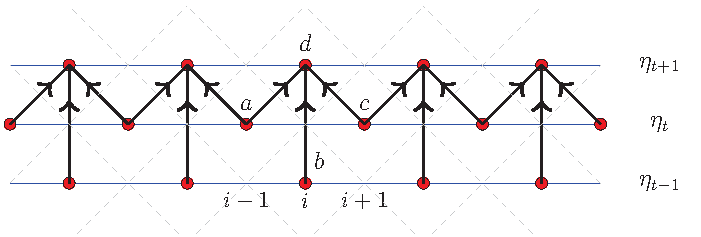
\includegraphics[scale=1]{Pictures/Figure_21.pdf} 
%%\begin{tikzpicture}
%\foreach \y in {0,1,2} \draw[blue] (-5,\y) -- (5,\y) ;
%\foreach \x in {-4,-2,\dots,4} \foreach \y in {0,2} {\draw [fill=red] (\x,\y) circle [radius=0.1] ;}
%\foreach \x in {-5,-3,\dots,5} \foreach \y in {1} {\draw [fill=red] (\x,\y) circle [radius=0.1] ;}
%\foreach \x in {-4,-2,\dots,4} \foreach \y in {2} {\draw[->-,thick] (\x,\y-2) -- (\x,\y) ;}
%%\foreach \x in {-4,-2,\dots,4} \foreach \y in {2} {\draw[->-,thick] (\x+1,\y-1) -- (\x,\y) ;}
%%\foreach \x in {-4,-2,\dots,4} \foreach \y in {2} {\draw[->-,thick] (\x-1,\y-1) -- (\x,\y) ;}
%\node at (6,2) {$\eta_{t+1}$};
%\node at (6,1) {$\eta_{t}$};
%\node at (6,0) {$\eta_{t-1}$};
%\node[above] at (-1,1.1) {$a$};
%\node[above right] at (0,0.1) {$b$};
%\node[above] at (1,1.1) {$c$};
%\node[above] at (0,2.1) {$d$};
%\node at (-1,-0.3) {\small{$i-1$}};
%\node at (0,-0.3) {\small{$i$}};
%\node at (1,-0.3) {\small{$i+1$}};
%\foreach \x in {-4,-2,\dots,0} {\draw [color=gray!50,dashed] (\x,-1) -- (\x+4,3) ;}
%\draw [color=gray!50,dashed] (-5,0) -- (-5+3,3) ;
%\draw [color=gray!50,dashed] (-2,-1) -- (-2-3,2) ;
%\foreach \x in{0,2,\dots,4} {\draw [color=gray!50,dashed] (\x,-1) -- (\x-4,3) ;}
%\draw [color=gray!50,dashed] (5,0) -- (5-3,3) ;
%\draw [color=gray!50,dashed] (2,-1) -- (2+3,2) ;
%\end{tikzpicture}
%%\end{center}
\caption{Illustration of the way $\eta_{t+1}$ is obtained from $\eta_{t}$ and $\eta_{t-1}$, using the transition kernel~$T$. The value $\eta_{t+1}(i)$ is equal to $d$ with probability $T(a,b,c;d)$, and conditionally on $\eta_{t}$ and $\eta_{t-1}$, the values $(\eta_{t+1}(i))_{i \in \Z_{t+1}}$ are independent.}\label{fig:def}
\end{figure}

Let us assume that initially, $(\eta_0,\eta_1)$ is distributed according to the uniform product measure $\lambda=\ber(1/2)^{\otimes \Z_0}\otimes\ber(1/2)^{\otimes \Z_1}$. Then, we can show that for any $t\in \NN$, $(\eta_t,\eta_{t+1})$ is also distributed according to $\lambda$. We will say that the PCA has an invariant \emph{Horizontal Zigzag Product Measure}. By stationarity, we can then extend the space-time diagram to a random field with values in $S^{\Z_{e}^2}$. The study of the space-time diagram shows that it has some peculiar properties, which we will precise in the next sections. In particular, it is quasi-reversible: if we reverse the direction of time, the random field corresponds to the stationary space-time diagram of another PCA. Furthermore, the PCA is ergodic: whatever the distribution of $(\eta_0,\eta_1)$, the distribution of $(\eta_t,\eta_{t+1})$ converges weakly to $\lambda$ (meaning that for any $n\in\NN$, the restriction of $(\eta_t,\eta_{t+1})$ to the cells of abscissa ranging between $-n$ and $n$ converges to a uniform product measure). For $q=r$, the stationary space-time diagram presents even more symmetries and directional reversibilities: it has the same distribution as if we had iterated the PCA in any other of the four cardinal directions. In addition, any straight line drawn along the space-time diagram is made of i.i.d. random variables, see Figure~\ref{fig:std} for an illustration.

We will show that this PCA belongs to a more general class of PCA that are all ergodic and for which the stationary space-time diagram share specific properties (independence, directional reversibility).

\begin{figure}
\begin{center}
\begin{tabular}{cc}
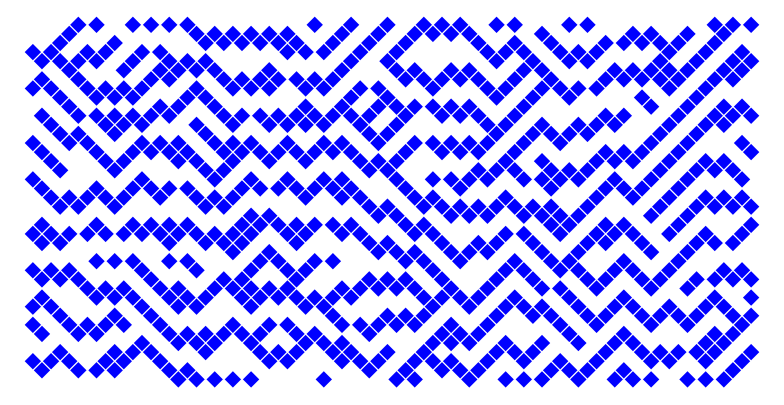
\includegraphics[scale=0.25]{Pictures/r=02,p=09.png} &
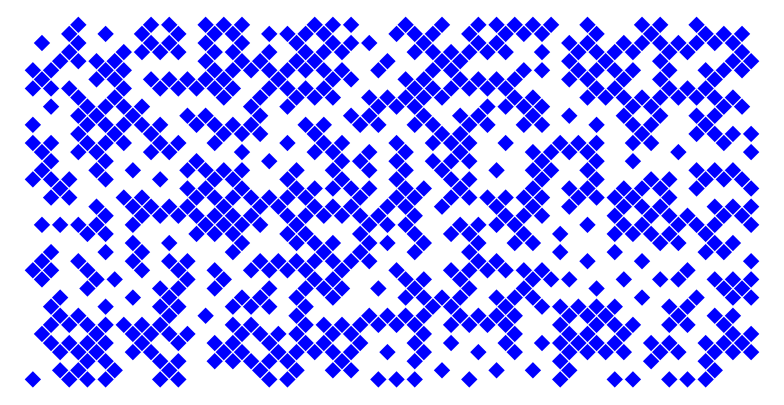
\includegraphics[scale=0.25]{Pictures/p=r=02.png} \\
$q=0.9$ and $r=0.2$ & $q=r=0.2$
\end{tabular}
\caption{Examples of portions of stationary space-time diagrams of the\break $8$-vertex PCA, for different values of the parameters. Cells in state $1$ are represented in blue, and cells in state $0$ are white.}\label{fig:std}
\end{center}
\end{figure}

\subsection{PCA with memory two and their invariant measures}

In this article, we only consider PCA with memory two for which the value of a given cell at time $t+1$ is drawn according to a distribution which is a function of the states of its two nearest neighbours at time $t$, and of its own state at time $t-1$. We thus introduce the following definition of transition kernel and of PCA with memory two.

\begin{definition}
Let $S$ be a finite set, called the \emph{alphabet}. A \emph{transition kernel} is a function $T$ that maps any $(a,b,c)\in S^3$ to a probability distribution on $S$. We denote by $T(a,b,c;\cdot)$ the distribution on $S$ which is the image of the triplet $(a,b,c)\in S^3$, so that: $\forall d\in S$, $T(a,b,c;d)\in [0,1]$ and $\sum_{d \in S} T(a,b,c;d)$=1.

A \emph{probabilistic cellular automaton (PCA) with memory two} of transition kernel $T$ is a Markov chain of order two $(\eta_t)_{t\geq 0}$ such that $\eta_t$ has values in $S^{\Z_t}$, and conditionally on $\eta_t$ and $\eta_{t-1}$, for any $i \in \Z_{t+1}$, $\eta_{t+1}(i)$ is distributed according to $T(\eta_t(i-1),\eta_{t-1}(i),\eta_{t}(i+1);\cdot)$, independently for different $i \in\Z_{t+1}$.
\end{definition}

By definition, if $(\eta_t(i-1),\eta_{t-1}(i),\eta_{t}(i+1))=(a,b,c)$, then $\eta_{t+1}(i)$ is equal to $d\in S$ with probability $T(a,b,c;d)$, see Figure~\ref{fig:def} for an illustration. We say that a PCA has \emph{positive rates} if its transition kernel $T$ is such that $\forall a,b,c,d\in S$, $T(a,b,c;d)>0$. One can consider a PCA of order 2 on $S$ as a PCA of order 1 on $S^2$, but the resulting PCA then does not have positive rates, which leads to significant difficulties. We thus introduce specific tools for the study of PCA of order 2.

Let $\mu$ be a distribution on $S^{\Z_{t-1}}\times S^{\Z_{t}}$, and let us introduce the two basis vectors $\vu=(-1,1)$ and $\vv=(1,1)$ of $\Z_{e}^2$. We denote by $\sigma_{\vv}(\mu)$ the distribution on $S^{\Z_{t}}\times S^{\Z_{t+1}}$ which is the image of $\mu$ by the mapping:
\[
\sigma_{\vv}: \left((x_k)_{k\in \Z_{t-1}},(y_l)_{l\in \Z_{t}}\right) \rightarrow \left((x_{k-1})_{k\in \Z_{t}},(y_{l-1})_{l\in \Z_{t+1}}\right).
\]

When considering the distribution $\mu$ as living on two consecutive horizontal lines of the lattice $\Z_{e}^2$, corresponding to times $t-1$ and $t$, the distribution $\sigma_{\vv}(\mu)$ thus corresponds to shifting $\mu$ by a vector $\vv=(1,1)$. Similarly, we denote by $\sigma_{\vv-\vu}(\mu)$ the distribution on $S^{\Z_{t-1}}\times S^{\Z_{t}}$ which is the image of $\mu$ by the application: $\sigma_{\vv-\vu}:\left((x_k)_{k\in \Z_{t-1}},(y_l)_{l\in \Z_{t}}\right) \rightarrow \left((x_{k-2})_{k\in \Z_{t-1}},(y_{l-2})_{l\in \Z_{t}}\right).$

For our specific context of PCA with memory two, we introduce the following definitions.

\begin{definition}\label{def:prob-inv}
Let $\mu$ be a probability distribution on $S^{\Z_{0}}\times S^{\Z_{1}}$.
\begin{itemize}
\item The distribution $\mu$ is said to be \emph{shift-invariant} if $\sigma_{\vv-\vu}(\mu)=\mu$.

\item The distribution $\mu$ on $S^{\Z_{0}}\times S^{\Z_{1}}$ is an \emph{invariant distribution} of a PCA with memory two if the PCA dynamics is such that: $(\eta_{0},\eta_{1}) \sim \mu \implies (\eta_{1},\eta_{2}) \sim \sigma_{\vv}(\mu).$

\end{itemize}
\end{definition}

By a standard compactness argument, one can prove that any PCA has at least one invariant distribution which is shift-invariant. In this article, we will focus on such invariant distributions. Note that if $\mu$ is both a shift-invariant measure and an invariant distribution of a PCA, then we also have $(\eta_{0},\eta_{1}) \sim \mu \implies (\eta_{1},\eta_{2}) \sim \sigma_{\vu}(\mu).$

\begin{defi}
Let $p$ be a distribution on $S$. The $p$-HZPM (for \emph{Horizontal Zigzag Product Measure}) on $S^{\Z_{t-1}}\times S^{\Z_{t}}$ is the distribution $\pi_p=p^{\otimes\Z_{t-1}}\otimes p^{\otimes\Z_t}$.
\end{defi}

Observe that we do not specify $t$ in the notation, since there will be no possible confusion. By Definition~\ref{def:prob-inv}, $\pi_p$ is invariant for a PCA if:
\[
(\eta_{t-1},\eta_t) \sim \pi_p \implies (\eta_{t},\eta_{t+1}) \sim \pi_p.
\]

\subsection{Stationary space-time diagrams and directional (quasi-)reversibility}\label{ssec:sstd}

Let $A$ be a PCA and $\mu$ one of its invariant measures. Let $G_k = (\eta_t(i) : t \in \{-k,\dots,k\}, i \in \ZZ_t)$ be a space-time diagram of $A$, started at time $t=-k$ under its invariant measure $\mu$, until time $t=k$. Then $(G_k)_{k\geq 0}$ induces a sequence of compatible measures on $\Z_{e}^2$ and, by Kolmogorov's extension theorem, defines a unique measure on $\Z_{e}^2$, that we denote by $\L(A,\mu)$.

\begin{defi}\label{def:std}
Let $A$ be a PCA and $\mu$ one of its invariant distributions which is shift-invariant. A random field $(\eta_t(i) : t \in \ZZ, i \in \ZZ_t)$ which is distributed according to $\L(A,\mu)$ is called a \emph{stationary space-time diagram} of $A$ taken under $\mu$.
\end{defi}

We will use the notation $G(A,\mu)$ to represent a stationary space-time diagram of $A$ taken under $\mu$, that is, a random field with distribution $\L(A,\mu)$.

We denote by $D_4$ the dihedral group of order $8$, that is, the group of symmetries of the square. We denote by $r$ the rotation of angle $\pi/2$ and by $h$ the horizontal reflection. We denote the vertical reflection by $v=r^2\circ h$, and the identity by $id$. For a subset $E$ of $D_4$, we denote by $\vect{E}$ the subgroup of $D_4$ generated by the elements of $E$.

\begin{defi}\label{def:rev}
Let $A$ be a positive-rates PCA, and let $\mu$ be an invariant measure of $A$ which is shift-invariant. For $g \in D_4$, we say that $(A,\mu)$ is \emph{$g$-quasi-reversible}, if there exists a PCA $A_g$ and a measure $\mu_g$ such that the associated stationary space time-diagrams satisfy
\[
{G(A,\mu) \eqd g^{-1} \circ G(A_g,\mu_g)}.
\]
In this case, the pair $(A_g,\mu_g)$ is the $g$-reverse of $(A,\mu)$. If, moreover, $(A_g,\mu_g)=(A,\mu)$, then $(A,\mu)$ is said to be \emph{$g$-reversible}.

For a subset $E$ of $D_4$, we say that $A$ is $E$-quasi-reversible (resp. $E$-reversible) if it is $g$-quasi-reversible (resp. $g$-reversible) for any $g\in E$.
\end{defi}

Classical definitions of quasi-reversibility and reversibility of PCA correspond to time-reversal, that are, $h$-quasi-reversibility and $h$-reversibility. Geometrically, the stationary space-time diagram $(A,\mu)$ is $g$-quasi-reversible if after the action of the isometry $g$, the random field has the same distribution as if we had iterated another PCA $A_g$ (or the same PCA $A$, in the reversible case). In particular, if $(A,\mu)$ is $r$-quasi-reversible (resp. $r^2$, $r^3$), it means that even if the space-time diagram is originally defined by an iteration of the PCA $A$ towards the North, it can also be described as the stationary space-time diagram of another PCA directed to the East (resp. to the South, to the West).

The stationary space-time diagram of a PCA (see Definition~\ref{def:std}) is a random field indexed by $\Z_{e}^2$. For a point $x=(i,t)\in\Z_{e}^2$, we will also use the notation $\eta(x)=\eta(i,t)=\eta_t(i)$, and for a family $L\subset\Z_{e}^2$, we define $\eta(L)=(\eta(x))_{x\in L}$.

The following Lemma~\ref{lem-std} proves that the space-time diagram of a positive-rate PCA characterizes its dynamics. Precisely, if two positive-rates PCA $A$ and $A'$ have the same space-time diagram (in law) taken under their respective invariant measures $\mu$ and $\mu'$, then $A=A'$ and $\mu=\mu'$.

\begin{lemm}\label{lem-std}
Let $(A,\mu)$ and $(A',\mu')$ be two positive-rates PCA with one of their invariant measure. Then, $\L(A,\mu) = \L(A',\mu') \implies (A,\mu) = (A',\mu').$
\end{lemm}

\begin{proof}
Let $G=G(A,\mu)=(\eta_t(i) : t \in \ZZ, i \in \ZZ_t)$ and $G'=G(A',\mu')=(\eta'_t(i) : t \in \ZZ, i \in \ZZ_t)$ be two space-time diagrams of law $\L(A,\mu)$ and $\L(A',\mu')$. By definition, $G|_{t=0,1} \sim \mu$ and $G'|_{t=0,1} \sim \mu'$. Since $G \eqd G'$, we obtain $\mu = \mu'$.

Let us denote $\mu(a,b,c)=\Pbb\left(\eta_1(-1) = a, \eta_0(0) = b, \eta_1(1) = c\right)$. As a consequence of the fact that $A$ has positive rates, we have $\forall (a,b,c) \in S^3, \mu(a,b,c)> 0$.
Thus, for any $a,b,c,d\in S,$ we have
\[
\Pbb\left(\eta_1(-1) = a, \eta_0(0) = b, \eta_1(1) = c, \eta_2(0) = d\right) = \mu(a,b,c) T(a,b,c;d) > 0.
\]
The same relation holds for $A'$ and as $G \eqd G'$, we obtain $\mu(a,b,c) T(a,b,c;d)= \mu'(a,b,c) T'(a,b,c;d).$ Since $\mu=\mu'$, we deduce that $T(a,b,c;d) = T'(a,b,c;d)$ for any $a,b,c,d\in S$. Hence, $A=A'$.
\end{proof}

By Lemma~\ref{lem-std}, if a PCA is $g$-quasi-reversible (see Definition~\ref{def:rev}), its $g$-reverse is thus unique. Let us now enumerate some easy results on quasi-reversible PCA and reversible PCA. Although the following proposition is quite straightforward, we are not aware of any reference formalizing the notion of directional reversibility and the properties below.

\begin{prop}\label{prop:obvious}
Let $A$ be a positive-rates PCA and let $\mu$ be one of its invariant measures.
\begin{enumerate}
\item \label{list2.7.1}$(A,\mu)$ is $\id$-reversible.
\item \label{list2.7.2}$(A,\mu)$ is $v$-quasi-reversible and the $v$-reverse PCA is defined by the transition kernel $T_v(c,b,a;d) = T(a,b,c;d)$.
\item \label{list2.7.3}For any $g \in D_4$, if $(A,\mu)$ is $g$-quasi-reversible, then its $g$-reverse $(A_g,\mu_g)$ is $g^{-1}$-quasi-reversible and $(A,\mu)$ is the $g^{-1}$-reverse of $(A_g,\mu_g)$.
\item \label{list2.7.4}If $(A,\mu)$ is $g$-quasi-reversible and $(A_g,\mu_g)$ is its $g$-reverse and if $(A_g,\mu_g)$ is $g'$-quasi-reversible and $(A_{g'g},\mu_{g'g})$ is its $g'$-reverse, then $(A,\mu)$ is $g' g$-quasi-reversible and $(A_{g'g},\mu_{g'g})$ is its $g' g$-reverse.
\item \label{list2.7.5}For any subset $E$ of $D_4$, if $(A,\mu)$ is $E$-reversible, then $(A,\mu)$ is $\vect{E}$-reversible.
\end{enumerate}
\end{prop}

\begin{rema}
Since $\vect{r,v}=D_4$, a consequence of the last point of Proposition~\ref{prop:obvious} is that if $(A,\mu)$ is $r$ and $v$-reversible, then it is $D_4$-reversible.
\end{rema}

Table~\ref{table:pres} presents a summary of the results that will be proven in the next sections, concerning PCA having a $p$-HZPM invariant distribution and their stationary space-time diagrams. For each possible (quasi-)reversibility behaviour, we give the conditions that the parameters of the PCA must satisfy (see Section~\ref{sec:rqrPCA} for details), and provide the number of degrees of freedom left by these equations, that is, the dimension of the corresponding submanifold of the parameter space (see Section~\ref{sec:dim}). In a similar fashion, Table~\ref{table:pres-HZMC} synthesized the main results about PCA having a Markovian invariant measure (see Section~\ref{sec:markov}).

%%A: la taille du tableau est problématique... tiny fait tenir dans la marge mais \scriptsize rend l'ensemble plus lisible...
%{\scriptsize
%%ou \tiny mais c'est trop petit
%~ \resizebox est parfait pour ça
\begin{table}
\caption{Summary of the characterization of (quasi-)reversible PCA having a $p$-HZPM invariant distribution. We denote by $n$ the cardinal of the alphabet $S$.}\label{table:pres}
\resizebox{0.95\textwidth}{!}{
\begin{tabular}{|c|c|c|}
\hline Conditions & Property & Dim. of the submanifold \\
on the parameters & of the PCA & (nb. of deg. of freedom)\\
\hline \hline
\begin{tabular}{c}
\myencadre{\begin{cond}\label{cond-pm}
$\forall a,c,d\in S$,\\ $p(d) = \sum_{b \in S} p(b) T(a,b,c;d)$%
\end{cond}}
\end{tabular}
&
\begin{tabular}{c}
$p$-HZPM invariant\\
$\{r^2,h\}$-quasi-reversible \\[0.2cm]
$T_{r^2}(c,d,a;b)=\frac{p(b)}{p(d)}T(a,b,c;d)$ \\[0.1cm]
$T_{h}(a,d,c;b)=\frac{p(b)}{p(d)}T(a,b,c;d)$
\end{tabular} & $n^2(n-1)^2$ \\
\hline
\begin{tabular}{c}
\Cond~\ref{cond-pm} + \\[0.15cm]
\myencadre{
\begin{cond}\label{cond:r1rev}
$\forall a,b,d \in S$,
\end{cond}\\ $p(d) = \sum_{c \in S} p(c) T(a,b,c;d)$}
\end{tabular} &
\begin{tabular}{c}
$r$-quasi-reversible\vspace{0.2cm} \\
$T_{r}(d,a,b;c)= \frac{p(c)}{p(d)}T(a,b,c;d)$
\end{tabular} & $n(n-1)^3$ \\
\hline
\begin{tabular}{c}
\Cond~\ref{cond-pm} + \\[0.15cm]
\myencadre{
\begin{cond}\label{cond:r3rev}
$\forall b,c,d \in S$
\end{cond},\\ $p(d) = \sum_{a \in S} p(a) T(a,b,c;d)$}
\end{tabular} &
\begin{tabular}{c}
$r^{-1}$-quasi-reversible \vspace{0.2cm}\\
$T_{r^{-1}}(b,c,d;a)=\frac{p(a)}{p(d)}T(a,b,c;d)$
\end{tabular} & $n(n-1)^3$ \\
\hline&&\\[-0.2em]
\begin{tabular}{c}
\Cond~\ref{cond-pm} + \Cond~\ref{cond:r1rev} + \Cond~\ref{cond:r3rev}
\end{tabular}%\foreach \y in {0,1,2} \draw[blue] (-5,\y) -- (5,\y) ;
%\foreach \x in {-4,-2,\dots,4} \foreach \y in {0,2} {\draw [fill=red] (\x,\y) circle [radius=0.1] ;}
%\foreach \x in {-5,-3,\dots,5} \foreach \y in {1} {\draw [fill=red] (\x,\y) circle [radius=0.1] ;}
%\foreach \x in {-4,-2,\dots,4} \foreach \y in {2} {\draw[->-,thick] (\x,\y-2) -- (\x,\y) ;}
%%\foreach \x in {-4,-2,\dots,4} \foreach \y in {2} {\draw[->-,thick] (\x+1,\y-1) -- (\x,\y) ;}
%%\foreach \x in {-4,-2,\dots,4} \foreach \y in {2} {\draw[->-,thick] (\x-1,\y-1) -- (\x,\y) ;}
%\node at (6,2) {$\eta_{t+1}$};
%\node at (6,1) {$\eta_{t}$};
%\node at (6,0) {$\eta_{t-1}$};
%\node[above] at (-1,1.1) {$a$};
%\node[above right] at (0,0.1) {$b$};
%\node[above] at (1,1.1) {$c$};
%\node[above] at (0,2.1) {$d$};
%\node at (-1,-0.3) {\small{$i-1$}};
%\node at (0,-0.3) {\small{$i$}};
%\node at (1,-0.3) {\small{$i+1$}};
%\foreach \x in {-4,-2,\dots,0} {\draw [color=gray!50,dashed] (\x,-1) -- (\x+4,3) ;}
%\draw [color=gray!50,dashed] (-5,0) -- (-5+3,3) ;
%\draw [color=gray!50,dashed] (-2,-1) -- (-2-3,2) ;
%\foreach \x in{0,2,\dots,4} {\draw [color=gray!50,dashed] (\x,-1) -- (\x-4,3) ;}
%\draw [color=gray!50,dashed] (5,0) -- (5-3,3) ;
%\draw [color=gray!50,dashed] (2,-1) -- (2+3,2) ;
%\end{tikzpicture}
%%\end{center}
& $D_4$-quasi-reversible & $(n-1)^4$ \\&&\\[-0.2em]
\hline \hline
\begin{tabular}{c}
\Cond~\ref{cond-pm} + \\[-0.1cm]
\test\encadre{$\forall a,b,c,d \in S$,\\
$T(a,b,c;d) = T(c,b,a;d)$}
\end{tabular} & $v$-reversible & $\displaystyle \frac{(n-1)^2n(n+1)}{2}$ \\
\hline%\foreach \y in {0,1,2} \draw[blue] (-5,\y) -- (5,\y) ;
%\foreach \x in {-4,-2,\dots,4} \foreach \y in {0,2} {\draw [fill=red] (\x,\y) circle [radius=0.1] ;}
%\foreach \x in {-5,-3,\dots,5} \foreach \y in {1} {\draw [fill=red] (\x,\y) circle [radius=0.1] ;}
%\foreach \x in {-4,-2,\dots,4} \foreach \y in {2} {\draw[->-,thick] (\x,\y-2) -- (\x,\y) ;}
%%\foreach \x in {-4,-2,\dots,4} \foreach \y in {2} {\draw[->-,thick] (\x+1,\y-1) -- (\x,\y) ;}
%%\foreach \x in {-4,-2,\dots,4} \foreach \y in {2} {\draw[->-,thick] (\x-1,\y-1) -- (\x,\y) ;}
%\node at (6,2) {$\eta_{t+1}$};
%\node at (6,1) {$\eta_{t}$};
%\node at (6,0) {$\eta_{t-1}$};
%\node[above] at (-1,1.1) {$a$};
%\node[above right] at (0,0.1) {$b$};
%\node[above] at (1,1.1) {$c$};
%\node[above] at (0,2.1) {$d$};
%\node at (-1,-0.3) {\small{$i-1$}};
%\node at (0,-0.3) {\small{$i$}};
%\node at (1,-0.3) {\small{$i+1$}};
%\foreach \x in {-4,-2,\dots,0} {\draw [color=gray!50,dashed] (\x,-1) -- (\x+4,3) ;}
%\draw [color=gray!50,dashed] (-5,0) -- (-5+3,3) ;
%\draw [color=gray!50,dashed] (-2,-1) -- (-2-3,2) ;
%\foreach \x in{0,2,\dots,4} {\draw [color=gray!50,dashed] (\x,-1) -- (\x-4,3) ;}
%\draw [color=gray!50,dashed] (5,0) -- (5-3,3) ;
%\draw [color=gray!50,dashed] (2,-1) -- (2+3,2) ;
%\end{tikzpicture}
%%\end{center}
\begin{tabular}{c}
\Cond~\ref{cond-pm} + \\[-0.1cm]
\test\encadre{$\forall a,b,c,d \in S$,\\
$p(b) T(a,b,c;d) = p(d) T(c,d,a;b)$}
\end{tabular} & $r^2$-reversible & $\displaystyle \frac{(n-1)^2n(n+1)}{2}$ \\
\hline
\begin{tabular}{c}
\Cond~\ref{cond-pm} + \\[-0.1cm]
\test\encadre{$\forall a,b,c,d \in S$,\\
$p(b) T(a,b,c;d) = p(d) T(a,d,c;b)$}
\end{tabular} & $h$-reversible & $\displaystyle \frac{n^3(n-1)}{2}$ \\
\hline

\begin{tabular}{c}
\Cond~\ref{cond-pm} + \\[0.1cm]
\test\encadre{$\forall a,b,c,d \in S$,\\
$T(a,b,c;d) = T(c,b,a;d)$ and \\
$p(b) T(a,b,c;d) = p(d) T(c,d,a;b)$}
\end{tabular} & $<r^2,v>$-reversible & $\displaystyle \frac{(n-1)n^2(n+1)}{4}$ \\
\hline

\begin{tabular}{c}
\Cond~\ref{cond-pm} + \\[-0.1cm]
\test\encadre{$\forall a,b,c,d \in S$,\\
$p(a) T(a,b,c;d) = p(d) T(b,c,d;a)$}
\end{tabular} & $\vect{r}$-reversible & $\displaystyle \frac{n(n-1)(n^2-3n+4)}{4}$ \\
\hline

\begin{tabular}{c}
\Cond~\ref{cond-pm} + \\[-0.1cm]
\test
\encadre{$\forall a,b,c,d \in S$,\\
$p(a) T(a,b,c;d) = p(d) T(d,c,b;a)$}
\end{tabular} & $<r \circ v>$-reversible & $\displaystyle \frac{(n-1)^2 (n^2-2n+2)}{2}$ \\
\hline
\begin{tabular}{c}
\Cond~\ref{cond-pm} + \\[0.1cm]
\test\encadre{$\forall a,b,c,d \in S$,\\
$p(a) T(a,b,c;d) = p(d) T(b,c,d;a)$ and\\
$T(a,b,c;d) = T(c,b,a;d)$}
\end{tabular} & $D_4$-reversible & $\displaystyle \frac{n(n-1)(n^2-n+2)}{8}$ \\
\hline
\end{tabular}}
\end{table}

{\scriptsize
\begin{table}
\caption{Summary of the characterization of (quasi-)reversible PCA having a $(F,B)$-HZMC invariant distribution.}\label{table:pres-HZMC}
\begin{tabular}{|c|c|}
\hline Conditions & Property \\
on the parameters & of the PCA \\
\hline \hline
\begin{tabular}{c}
\myencadre[6.9cm]{\begin{cond}\label{cond:DU-HZMC}
$\forall a,c,d\in S$,\\ $F(a;d) B(d;c) = \sum_{b \in S} B(a;b) F(b;c) T(a,b,c;d)$%
\end{cond}}
\end{tabular}&
\begin{tabular}{c}
$(F,B)$-HZMC invariant\\
$\{r^2,h\}$-quasi-reversible \vspace{0.2cm}\\
$T_{r^2}(c,d,a;b)= \frac{B(a;b)F(b;c)}{F(a;d)B(d;c)} T(a,b,c;d)$ \vspace{0.1cm}\\
$T_{h}(a,d,c;b) = \frac{B(a;b)F(b;c)}{F(a;d)B(d;c)} T(a,b,c;d)$
\end{tabular}\\
\hline
\begin{tabular}{c}
\Cond~\ref{cond:DU-HZMC} + \\[0.15cm]
\myencadre{
\begin{cond}\label{cond:r1DU}
$\forall a,c,d \in S$,
\end{cond}\\ $F(a;d) = \sum_{c \in S} F(b;c) T(a,b,c;d)$}
\end{tabular} &
\begin{tabular}{c}
$r$-quasi-reversible\vspace{0.2cm} \\
$T_{r}(d,a,b;c)= \frac{F(b;c)}{F(a;d)}T(a,b,c;d)$
\end{tabular} \\
\hline
\begin{tabular}{c}
\Cond~\ref{cond:DU-HZMC} + \\[0.15cm]
\myencadre[6cm]{
\begin{cond}\label{cond:r3DU}
$\forall b,c,d \in S$,\\ $\frac{\rho(d)}{\rho(c)} B(d;c) = \sum_{a \in S} \frac{\rho(a)}{\rho(b)} B(a;b) T(a,b,c;d)$
\end{cond}}
\end{tabular} &
\begin{tabular}{c}
$r^{-1}$-quasi-reversible \vspace{0.2cm}\\
$T_{r^{-1}}(b,c,d;a)=\frac{\rho(a) \rho(c) B(a;b)}{\rho(b) \rho(d) B(d;c)} T(a,b,c;d)$
\end{tabular}\\
\hline
\end{tabular}
\end{table}}

\section{Invariant product measures and ergodicity}\label{sec:cond_ergo}

In this section, we lay the groundwork for the study of PCA with memory two having an invariant measure with a product form. First, Theorem~\ref{theo:gen0} gives the necessary and sufficient condition for a PCA to have a $p$-HZPM invariant distribution (\Cond~\ref{cond-pm}). This condition will be extensively used in the continuation of the article. We then prove that any PCA satisfying this condition is ergodic, meaning that whatever the initial distribution for times $t=0$ and $t=1$, when iterating the dynamics, the PCA converges to the product measure of parameter $p$. Finally, we show that the stationary space-time diagrams of PCA having a $p$-HZPM invariant distribution share the following property: not only all the horizontal zigzag lines are distributed according to the product measure of parameter $p$, but also more general zigzag lines (in the sense of Definition~\ref{def:zigzagpolyline}).

\subsection{Conditions for having an invariant HZPM}

To start with, next Theorem~\ref{theo:gen0} gives a characterization of PCA with memory two having a $p$-HZPM invariant distribution.

\begin{theo}\label{theo:gen0}
Let $A$ be a positive-rates PCA with transition kernel $T$, and let $p$ be a probability vector on $S$. The $p$-HZPM distribution $\pi_p$ is invariant for $A$ if and only if:

\textnormal{\begin{conddd}{cond-pm}
for any $a,c,d\in S$, $p(d) = \sum_{b \in S} p(b) T(a,b,c;d)$.
\end{conddd}}
\end{theo}

Note that since $A$ has positive rates, if $\pi_p$ is invariant for $A$, then the vector $p$ has to be positive. For a positive probability vector $p$ on $S$, we define $\triang{S}{p}$ as the set of positive-rates PCA for which the measure $\pi_p$ is invariant. We denote by $\triangE{S}$ the set of all positive-rates PCA with set of symbols $S$ having an invariant $p$-HZPM, for some positive probability vector $p$ on $S$.

As an immediate consequence of Theorem~\ref{theo:gen0}, one obtains the following result.

\begin{coro}\label{theo:gen}
Let $A$ be a positive-rates PCA with transition kernel $T$. Then, $A\in \triangE{S}$ if and only if for any $a,c \in S$, the left eigenspace $E_{a,c}$ of matrices $\left(T(a,b,c;d)\right)_{b,d \in S}$ related to the eigenvalue~$1$ is the same. In that case, the invariant HZPM is unique: it is the measure $\pi_p$ defined by the unique vector $p$ such that $E_{a,c} = \text{Vect}(p)$ for all $a,c\in S$ and $\sum_{b \in S} p(b) =1$.
\end{coro}

\begin{proof}[Proof of Theorem~\ref{theo:gen0}]
Let $p$ be a positive vector such that $\pi_p$ is invariant by $A$ and assume that $(\eta_{t-1},\eta_t) \sim \pi_p$. Then, on the one hand, since $\pi_p$ is invariant by $A$, we have
\begin{equation*}
\Pbb\left(\eta_{t}(i-1)=a, \eta_{t+1}(i) = d, \eta_{t}(i+1) = c\right) = p(a) p(c) p(d).
\end{equation*}
And on the other hand, by definition of the PCA,
\begin{equation*}
\Pbb\left(\eta_{t}(i-1)=a, \eta_{t+1}(i) = d, \eta_{t}(i+1) = c\right) = \sum_{b\in S} p(a) p(b) p(c) T(a,b,c;d).
\end{equation*}
\Cond~\ref{cond-pm} follows.

Conversely, assume that \Cond~\ref{cond-pm} is satisfied, and that $(\eta_{t-1},\eta_t) \sim \pi_p$. For some given choice of $n\in\Z_{t}$, let us denote: $X_i=\eta_{t-1}(n+1+2i), Y_i=\eta_{t}(n+2i), Z_i=\eta_{t+1}(n+1+2i),$ for $i\in \Z$, see Figure~\ref{fig:hzpm_proof} for an illustration. Then, for any $k\geq 1$, we have
\begin{multline*}
\Pbb\big((Y_i)_{0\leq i\leq k}= (y_i)_{0\leq i\leq k}, (Z_i)_{0\leq i\leq k-1}=(z_i)_{0\leq i\leq k-1}\big) \\
\begin{aligned}
&= \sum_{(x_i : 0\leq i\leq k-1)}\!\! \Pbb\left((X_i)_{0\leq i\leq k}=(x_i)_{0\leq i\leq k-1}, (Y_i)_{0\leq i\leq k}=\!(y_i)_{0\leq i\leq k}\right) \prod_{i=0}^{k-1} T(y_i,x_{i},y_{i+1};z_i)\\
&= \sum_{(x_i : 0\leq i\leq k-1)} \prod_{i=0}^{k-1} p(x_i) \prod_{i=0}^{k} p(y_i) \prod_{i=0}^{k-1} T(y_i,x_{i},y_{i+1};z_i) \\
&= \prod_{i=0}^{k} p(y_i) \prod_{i=0}^{k-1} \sum_{x_i\in S} p(x_i)T(y_i,x_{i},y_{i+1};z_i) \\
&= \prod_{i=0}^{k} p(y_i) \prod_{i=0}^{k-1} p(z_i) \text{ by \Cond~\ref{cond-pm}, thus, } \pi_p \text{ is invariant by } A.\mathrlap{\mkern 157mu\qed}
\end{aligned}
\end{multline*}
\let\qed\relax
\end{proof}

\begin{figure}[!h]
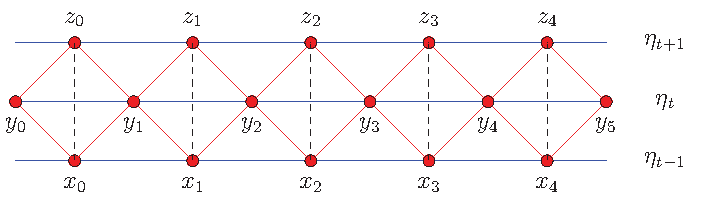
\includegraphics{Pictures/Figure_31.pdf} 
%%\begin{tikzpicture}
%%\foreach \y in {0,1,2} \draw[blue] (-5,\y) -- (5,\y) ;
%%\foreach \x in {-4,-2,\dots,4} \foreach \y in {0,2} {\draw [fill=red] (\x,\y) circle [radius=0.1] ;}
%%\foreach \x in {-5,-3,\dots,5} \foreach \y in {1} {\draw [fill=red] (\x,\y) circle [radius=0.1] ;}
%%\foreach \x in {-4,-2,\dots,4} \foreach \y in {2} {\draw[dashed] (\x,\y-2) -- (\x,\y) ;}
%\foreach \x in {-3,-1,\dots,3} \foreach \y in {1} {\draw[red] (\x-1,\y-1) -- (\x,\y) -- (\x+1,\y-1); \draw[red] (\x-1,\y+1) -- (\x,\y) -- (\x+1,\y+1);}
%\draw[red] (-5,1) -- (-4,2) ; \draw[red] (-5,1) -- (-4,0) ; \draw[red] (5,1) -- (4,0) ; \draw[red] (5,1) -- (4,2) ;
%\foreach \x in {0,1,\dots,4} \foreach \y in {0} {\node at (2*\x-4,\y-0.4) {$x_{\x}$};}
%\foreach \x in {0,1,\dots,4} \foreach \y in {2} {\node at (2*\x-4,\y+0.4) {$z_{\x}$};}
%\foreach \x in {0,1,\dots,5} \foreach \y in {1} {\node at (2*\x-4-1,\y-0.4) {$y_{\x}$};}
%\node at (6,2) {$\eta_{t+1}$};
%\node at (6,1) {$\eta_{t}$};
%\node at (6,0) {$\eta_{t-1}$};
%%\end{tikzpicture}
\caption{Illustration of the proof of Theorem~\ref{theo:gen0}.}\label{fig:hzpm_proof}
\end{figure}




As a consequence of Corollary~\ref{theo:gen}, $A\in\triangE{S}$ if and only if $A\in\triang{S}{p}$ for the unique $p$ given by the corollary.





\subsection{Ergodicity}

\begin{theo}\label{theo:ergo}
If $A\in \triangE{S}(p)$, then, $A$ is ergodic. Precisely, for any distribution of $(\eta_0, \eta_1)$, the distribution of $(\eta_t,\eta_{t+1})$ converges weakly to $\pi_p$.
\end{theo}

\begin{proof}
The proof we propose is inspired from~\cite{vasilyev}, see also~\cite{dobrushin} and \cite{marco_cie}. Let us fix some boundary conditions $(\ell, r)\in S^2$. Then, for any $k\geq 0$, the transition kernel $T$ induces a Markov chain on $S^{2k+1}$, such that the probability of a transition from the sequence $(a_0,b_0,a_1,b_1,\ldots, b_{k-1},a_{k})\in S^{2k+1}$ to a sequence $(a'_0,b'_0,a'_1,b'_1,\ldots, b'_{k-1},a'_{k})\in S^{2k+1}$ is given by:
\begin{multline*}
P_k^{(\ell,r)}\big((a_0,b_0,a_1,b_1,\ldots, b_{k-1},a_{k}), (a'_0,b'_0,a'_1,b'_1,\ldots, b'_{k-1},a'_{k})\big)\\
\begin{aligned}
& =T(\ell, a_0, b_0;a'_0)T(a'_0,b_0,a_1;b'_0)T(b_0, a_1, b_1;a'_1)\cdots T(b_{k-1},a_{k},r;a'_k)\\
& = T(\ell, a_0, b_0;a'_0)T(b_{k-1},a_{k},r;a'_k)\prod_{i=1}^{k-1}T(b_{i-1}, a_i, b_{i+1};a'_i)\prod_{i=0}^{k-1}T(a'_{i}, b_i, a'_{i+1};b'_i).
\end{aligned}
\end{multline*}
We refer to Figure~\ref{fig:ergo_proof} for an illustration. Let us observe that the restriction\linebreak $\pi^k_p=p^{\otimes 2k+1}$ of the $p$-HZPM is left invariant by this Markov chain. This is an easy consequence of \Cond~\ref{cond-pm}. For any $(\ell,r)\in S^2$, the transition kernel $P^{(\ell,r)}$ is positive. Therefore, there exists $\theta_{(\ell,r)}<1$ such that for any probability distributions $\nu, \nu'$ on $S^{2k+1}$, we have
\[
\left\|P_k^{(\ell,r)}\nu-P_k^{(\ell,r)}\nu'\right\|_1\leq \theta_k^{(\ell,r)} \|\nu-\nu'\|_1,
\]
the above inequality being true in particular for $\theta_k^{(\ell,r)}=1-\varepsilon_k^{(\ell,r)}$, where:
\[
\varepsilon_k^{(\ell,r)}=\min\{P_k^{(\ell,r)}(x,y) \, : \; x,y\in S^{2k+1}\}.
\]
Let us set $\theta_k=\max\{\theta_k^{(\ell,r)} \, : \; (\ell,r)\in S^2\}$. It follows that for any sequence $(\ell_t,r_t)_{t\geq 0}$ of elements of $S^2$, we have
\[
\left\|P_k^{(\ell_{t-1},r_{t-1})}\cdots P_k^{(\ell_{1},r_{1})}P_k^{(\ell_{0},r_{0})}\nu-P_k^{(\ell_{t-1},r_{t-1})}\cdots P_k^{(\ell_{1},r_{1})}P_k^{(\ell_{0},r_{0})}\nu'\right\|_1\leq \theta^t \|\nu-\nu'\|_1.
\]
In particular, for $\nu'=\pi^k_p$, we obtain that for any distribution $\nu$ on $S^{2k+1}$ and any sequence $(\ell_t,r_t)_{t\geq 0}$ of elements of $S^2$, we have
\[
\left\|P_k^{(\ell_{t-1},r_{t-1})}\cdots P_k^{(\ell_{1},r_{1})}P_k^{(\ell_{0},r_{0})}\nu-\pi^k_p\right\|_1\leq 2\theta^t.
\]
Let now $\mu$ be a distribution on $S^{\Z_0\cup\Z_1}$, and let $k\geq 0$. When iterating $A$, the\linebreak distribution $\mu$ induces a random sequence of symbols $\ell_t=\eta_{2t+1}(-(2k+1))$ and $r_t=\eta_{2t+1}(2k+1)$. Let us denote by $\nu_t$ the distribution of the sequence $(\eta_{2t}(-2k),\linebreak \eta_{2t+1}(-2k+1),\eta_{2t}(-2k+2),\ldots,\eta_{2t}(2k-2),\eta_{2t+1}(2k-1),\eta_{2t}(2k))$, and let $\pi^{2k}_p=p^{\otimes 4k+1}$. We have
\[
\forall t\geq\!0,\, \|\nu_t-\pi^{2k}_p\|_1\leq\! \max_{(\ell_0,r_0)\ldots (\ell_{t-1},r_{t-1})\in S^2} \left\|P_{2k}^{(\ell_{t-1},r_{t-1})}\ldots P_{2k}^{(\ell_{1},r_{1})}P_{2k}^{(\ell_{0},r_{0})}\nu_0-\pi^{2k}_p\right\|_1\!\leq 2\theta^t.
\]
This concludes the proof.
\end{proof}

\begin{figure}
\begin{center}
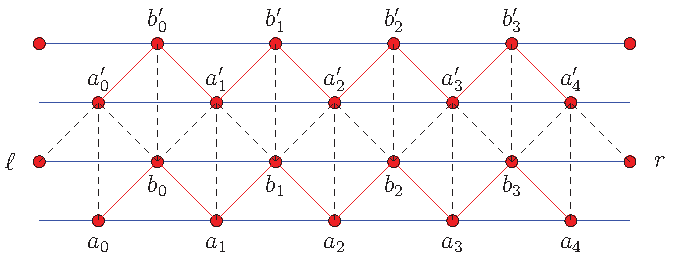
\includegraphics{Pictures/Figure_32.pdf} 
%%\begin{tikzpicture}
%%\foreach \y in {0,1,2, 3} \draw[blue] (-5,\y) -- (5,\y) ;
%%\foreach \x in {-4,-2,\dots,4} \foreach \y in {0,2} {\draw [fill=red] (\x,\y) circle [radius=0.1] ;}
%%\foreach \x in {-5,-3,\dots,5} \foreach \y in {1,3} {\draw [fill=red] (\x,\y) circle [radius=0.1] ;}
%%\foreach \x in {-4,-2,\dots,4} \foreach \y in {2} {\draw[dashed] (\x,\y-2) -- (\x,\y) ;}
%%\foreach \x in {-3,-1,\dots,3} \foreach \y in {3} {\draw[dashed] (\x,\y-2) -- (\x,\y) ;}
%%\foreach \x in {-4,-2,\dots,4} \foreach \y in {2} {\draw[dashed] (\x+1,\y-1) -- (\x,\y) ;}
%%\foreach \x in {-4,-2,\dots,4} \foreach \y in {2} {\draw[dashed] (\x-1,\y-1) -- (\x,\y) ;}
%%\foreach \x in {-3,-1,\dots,3} \foreach \y in {1,3} {\draw[red] (\x-1,\y-1) -- (\x,\y) ;}
%%\foreach \x in {-3,-1,\dots,3} \foreach \y in {1,3} {\draw[red] (\x+1,\y-1) -- (\x,\y) ;}
%%\node at (5.5,1) {$r$};
%%\node at (-5.5,1) {$\ell$};
%%\foreach \x in {0,1,\dots,4} \foreach \y in {0} {\node at (2*\x-4,\y-0.4) {$a_{\x}$};}
%%\foreach \x in {0,1,\dots,4} \foreach \y in {2} {\node at (2*\x-4,\y+0.4) {$a'_{\x}$};}
%%\foreach \x in {0,1,\dots,3} \foreach \y in {1} {\node at (2*\x-3,\y-0.4) {$b_{\x}$};}
%%\foreach \x in {0,1,\dots,3} \foreach \y in {3} {\node at (2*\x-3,\y+0.4) {$b'_{\x}$};}
%%\end{tikzpicture}
\end{center}\caption{Illustration of the proof of Theorem~\ref{theo:ergo}.}\label{fig:ergo_proof}
\end{figure}

\subsection{First properties of the space-time diagram}

Let us now focus on the space-time diagram $G(A,\pi_p)$ of a PCA $A\in\triang{S}{p}$, taken under its unique invariant measure $\pi_p$. By definition, any horizontal line of that space-time diagram is i.i.d. The following proposition extends this result to other types of lines.

\begin{defi}\label{def:zigzagpolyline}
A \emph{zigzag polyline} is a sequence $(i,t_i)_{m_1\leq i\leq m_2}\in \Z_{e}^2$ such that for any $i\in\{m_1,\ldots, m_2\}$, $(t_{i+1}-t_i)\in\{-1,1\}$.
\end{defi}

\begin{prop}\label{prop:ind}
Let $A \in \triang{S}{p}$ be a PCA of stationary space-time diagram $G(A,\pi_p)=(\eta_t(i) : t \in \ZZ, i \in \ZZ_t)$. For any zigzag polyline $(i,t_i)_{m_1\leq i\leq m_2}$, we have $(\eta_{t_i}(i) : i \in \{m_1,\ldots,m_2\}) \sim \mathcal{B}(p)^{\otimes (m_2-m_1+1)}$.
\end{prop}

Observe that Proposition~\ref{prop:ind} implies that (bi-)infinite zigzag polylines are also made of i.i.d. random variables with distribution $p$.

\begin{proof}
The proof is done by induction on $T = \max(t_i) - \min(t_i)$. If $T = 1$, then the zigzag polyline is an horizontal zigzag, and since $A \in \triang{S}{p}$, the result is true.

Now, suppose that the result is true for any zigzag polyline such that $\max(t_i)-\min(t_i) = T$, and consider a zigzag polyline $(i,t_i)_{m_1\leq i\leq m_2}$ such that $\max(t_i) - \min(t_i) = T+1$. Then, there exists $t$ such that $\min(t_i) = t$ and $\max(t_i) =t+T+1$. Let $M = \{i \in \{m_1,\ldots,m_2\} : t_i = t+T+1\}$. For any $i \in M$, we have $t_{i\pm 1} = t+T$ (we assume that $m_1,m_2\notin M$, even if it means extending the line). So, by induction, we have $(\eta(i,t_i - 2\ \ind{i \in M}) : i \in \{m_1,\ldots,m_2\}) \sim \mathcal{B}(p)^{\otimes (m_2-m_1+1)}$. For any $(a_i)_{m_1 \leq i \leq m_2}\in S^{m_2-m_1+1}$, we have
\begin{align*}
&\Pbb\left(\eta(x_i,t_i) = a_i : m_1 \leq i \leq m_2\right)\\
& = \sum_{(b_i : i \in M) \in S^{M}} \!\!\Pbb\big(\{\eta(i,t_i) \Mk=\Mk a_i\!:\!i \Mk\notin\Mk M\},\{\eta(i,t_i\Mk-\Mk2) \Mk=\Mk b_i\!:\!i \Mk\in\Mk M\}\big) \prod_{i \in M} T(a_{i-1},b_i,a_{i+1} ; a_i) \\
& = \sum_{(b_i : i \in M) \in S^{M}} \prod_{i \notin M} p(a_i) \prod_{i \in M} p(b_i) T(a_{i-1},b_i,a_{i+1} ; a_i) \\
& = \prod_{i \notin M} p(a_i) \prod_{i \in M} \sum_{b_i \in S} p(b_i) T(a_{i-1},b_i,a_{i+1} ; a_i) = \prod_{i =m_1}^{m_2} p(a_i).\mathrlap{\mkern 185mu\qed}
\end{align*}
\let\qed\relax
\end{proof}
%% régler le problème avec un alignement à droite. & ou mkern mu
\section{Directional (quasi-)reversibility of PCA having an invariant product measure} \label{sec:rqrPCA}

We now explore the directional reversibility and quasi-reversibility properties of PCA having an invariant $p$-HZPM. First, for any transformation $g$ of the dihedral group $D_4$, we give the necessary and sufficient condition under which the PCA is $g$-quasi-reversible or $g$-reversible, thus proving the results that were announced in Table~\ref{table:pres}. We then present some further properties of the stationary space-time diagrams that hold in this context, beyond Proposition~\ref{prop:ind}. Finally, these results will allow us to exhibit a family of PCA having an invariant measure that can be computed explicitly, although it does not have a product form or a Markovian one.

\subsection{(Quasi-)reversible PCA with invariant \texorpdfstring{$p$}{p}-HZPM}\label{sec:qrPCAinv}
In this section, we characterize PCA of $\triang{S}{p}$ that are $g$-quasi-reversible, for each possible $g\in D_4$. Let $A\in\triang{S}{p}$, and $g\in D_4$. From the transition kernel $T$ of $A$, we define a map $T_g: S^3 \times S\to \mathbb R_+$ by:
\[
\forall a,b,c,d\in S, \quad T_g(g(a,b,c);g(d))\isdef\frac{p(g(d))}{p(d)}T(a,b,c;d),
\]
where in the above expression, we use some abuse of notation when denoting by $g(a,b,c)$ and $g(d)$ the images of the vertices by the permutation induced by the transformation $g\in D_4$ (see~Figure~\ref{fig:def}). For example, in the case where $g=r$, we have $g(a,b,c)=(d,a,b)$, $g(d)=c$, and the expression above stands for:
\[
\forall a,b,c,d\in S, \quad T_r(d,a,b;c)\isdef\frac{p(c)}{p(d)}T(a,b,c;d).
\]
The expressions of $T_{r^2}, T_{h},$ and $T_{r^{-1}}$ can be found in Table~\ref{table:pres}.

Observe that $T_g$ is not necessarily a transition kernel. For example, $T_r$ is a transition kernel if and only if:
\[
\forall a,b,d\in S, \quad \sum_{c\in S} \frac{p(c)}{p(d)}T(a,b,c;d)=1,
\]
which is equivalent to \Cond~\ref{cond:r1rev}, see again Table~\ref{table:pres}. Analogously, $T_{r^{-1}}$ is a transition kernel if and only if \Cond~\ref{cond:r3rev} is satisfied. And it appears that as soon as a PCA belongs to $\triang{S}{p}$, $T_{r^2}$ and $T_h$ are transition kernels, since \Cond~\ref{cond-pm} is satisfied.

\begin{theo}\label{theo:referee}
A PCA $A \in \triang{S}{p}$ of transition kernel $T$ is $g$-quasi-reversible if and only if $T_g$ is a transition kernel. In that case, $T_g$ is the transition kernel of the $g$-reverse $A_g$ of $A$.
\end{theo}

Before proving Theorem~\ref{theo:referee}, let us present two corollaries that derive from it. First, the next result is a direct consequence of Theorem~\ref{theo:referee}.

\begin{corollary}\label{cor:reversibility}
Any PCA $A \in \triang{S}{p}$ is $r^2$-quasi-reversible and $h$-quasi-reversible.
\end{corollary}

For any stationary Markov chain, we can define a time-reversed chain, which still has the Markov property. But in general, the time-reversed chain of a stationary PCA is no more a PCA. Indeed, nothing ensures that for the time-reversed process, the states of different cells are independently distributed, conditionally on the states of their neighbours at the previous time step. So, it is restrictive to ask that the time reversal of the stationary Markov chain associated to a PCA of transition kernel $T$ is still distributed according to some transition kernel $T'$. Here, Corollary~\ref{cor:reversibility} shows that any PCA in $\triang{S}{p}$ is $r^2$-quasi-reversible, which means that the time-reversed chain of a PCA of $\triang{S}{p}$ is still a PCA with memory two, which furthermore belongs to $\triang{S}{p}$, since it preserves the measure $\pi_p$.

We also have the following characterization of reversible PCA.

\begin{coro}\label{theo:rev}
Let $A \in \triang{S}{p}$ and $g\in D_4$. The PCA $A$ is $g$-reversible iff $T_g=T$.
\end{coro}

\begin{proof}[Proof of Corollary~\ref{theo:rev}]
By Theorem~\ref{theo:referee}, $A$ is $g$-quasi-reversible iff $T_g$ is a transition kernel. It is furthermore reversible if $T_g=T$. Since $T$ is obviously a transition kernel, $A$ is $g$-reversible iff $T_g=T$.
\end{proof}

As a direct consequence, we obtain easily all the conditions for reversibility that are given in Table~\ref{table:pres}.

Let us now prove Theorem~\ref{theo:referee}. We begin the proof with the case $g=r^2$. The cases $g=\id$ and $g=v$ are obvious by Proposition~\ref{prop:obvious}, and the case $g=h$ will directly follow from the case $g=r^2$.



\begin{proof}[Proof of Theorem~\ref{theo:referee}, case $g=r^2$]
If $A\in\triang{S}{p}$, its transition kernel $T$ satisfies \Cond~\ref{cond-pm}, and thus, $T_{r^2}$ is a transition kernel. It only remains to prove that $A$ is indeed $r^{2}$-quasi-reversible, and that $T_{r^2}$ is the transition kernel of the $r^2$-reverse of $A$.



For some given choice of $n\in\Z_{t}$, let us denote again: $X_i=\eta_{t-1}(n+1+2i)$,\linebreak $Y_i=\eta_{t}(n+2i)$, $Z_i=\eta_{t+1}(n+1+2i)$, for $i\in \Z$, see Figure~\ref{fig:hzpm_proof}.

%\noindent
The following computation proves the result wanted.
\begin{multline*}
\Pbb\big((X_i)_{0\leq i\leq k} = (x_i)_{0\leq i\leq k} |(Y_i)_{0\leq i\leq k+1} = (y_i)_{0\leq i\leq k+1}, (Z_i)_{0\leq i\leq k} = (z_i)_{0\leq i\leq k}\big)\\
\begin{aligned}
&=\frac{\Pbb\big((X_i)_{0\leq i\leq k} = (x_i)_{0\leq i\leq k},(Y_i)_{0\leq i\leq k+1} = (y_i)_{0\leq i\leq k+1}, (Z_i)_{0\leq i\leq k} = (z_i)_{0\leq i\leq k}\big)}{\Pbb\big((Y_i)_{0\leq i\leq k+1} = (y_i)_{0\leq i\leq k+1}, (Z_i)_{0\leq i\leq k} = (z_i)_{0\leq i\leq k}\}\big)}\\
&=\frac{p(y_0) \prod_{i=0}^k p(x_i)p(y_{i+1}) T(y_i,x_i,y_{i+1};z_i)}{p(y_{0}) \prod_{i=0}^k p(z_i) p(y_{i+1})}\\
&=\prod_{i=0}^k \frac{p(x_i)}{p(z_i)} T(y_i,x_i,y_{i+1};z_i)\\
&=\prod_{i=0}^k T_{r^2}(y_{i+1},z_i,y_i ; x_i). \mathrlap{\mkern 373mu\qed}
\end{aligned}
\end{multline*}
\let\qed\relax
\end{proof}

Now, we will characterize PCA in $\triangE{S}(p)$ that are $r$-quasi-reversible.

We give now the proof of Theorem~\ref{theo:referee} in the case $g=r$. The case $g=r^{-1}$ is similar and the cases $g=r\circ v, g=r^{-1}\circ v$ then follow.

\goodbreak
\begin{proof}[Proof of Theorem~\ref{theo:referee}, case $g=r$]
%\begin{itemize}
%\item[$\bullet$]
Let us first prove that if $A$ is $r$-quasi-reversible, then \Cond~\ref{cond:r1rev} is satisfied and the transition kernel $\tilde T$ of the $r$-reverse $A_r$ of $A$ is equal to $T_r$. Let us recall the notations $\vu=(-1,1)$ and $\vv=(1,1)$. Since $A \in \triang{S}{p}$, for any $x \in \Z_{e}^2$ and $a,b,c,d \in S$, we have
\begin{align*}
\Pbb\left(\eta(x+\vu) = a, \eta(x) = b, \eta(x + \vv) = c, \eta(x+\vu+\vv) = d\right) = p(a) p(b) p(c) T(a,b,c;d).
\end{align*}
Hence, the transition kernel $\tilde T$ of $A_r$ satisfies:
\begin{equation}
\begin{aligned}
\tilde T(d,a,b;c)& = \Pbb\left(\eta(x + \vv) = c | \eta(x + \vu) = a, \eta(x) = b, \eta(x + \vu + \vv) = d\right) \\
& = \frac{p(a) p(b) p(c) T(a,b,c;d)}{\sum_{c'\in S} p(a) p(b) p(c') T(a,b,c';d)}  \\
& = \frac{p(c) T(a,b,c;d)}{\sum_{c'\in S} p(c') T(a,b,c';d)}. \label{eq:uniquerev}
\end{aligned}
\end{equation}

\begin{figure}[!h]
\begin{center}
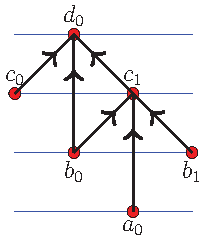
\includegraphics{Pictures/Figure_41.pdf} 
%%\begin{tikzpicture}[scale=1]
%%\foreach \y in {0,1,2,3} \draw[blue] (-2,\y) -- (1,\y) ;
%%\foreach \x in {0} \foreach \y in {0} {\draw [fill=red] (\x,\y) circle [radius=0.1] ;}
%%\foreach \x in {-1,1} \foreach \y in {1} {\draw [fill=red] (\x,\y) circle [radius=0.1] ;}
%%\foreach \x in {-2,0} \foreach \y in {2} {\draw [fill=red] (\x,\y) circle [radius=0.1] ;}
%%\foreach \x in {-1} \foreach \y in {3} {\draw [fill=red] (\x,\y) circle [radius=0.1] ;}
%%\foreach \x in {0} \forea%\foreach \y in {0,1,2} \draw[blue] (-5,\y) -- (5,\y) ;
%\foreach \x in {-4,-2,\dots,4} \foreach \y in {0,2} {\draw [fill=red] (\x,\y) circle [radius=0.1] ;}
%\foreach \x in {-5,-3,\dots,5} \foreach \y in {1} {\draw [fill=red] (\x,\y) circle [radius=0.1] ;}
%\foreach \x in {-4,-2,\dots,4} \foreach \y in {2} {\draw[->-,thick] (\x,\y-2) -- (\x,\y) ;}
%%\foreach \x in {-4,-2,\dots,4} \foreach \y in {2} {\draw[->-,thick] (\x+1,\y-1) -- (\x,\y) ;}
%%\foreach \x in {-4,-2,\dots,4} \foreach \y in {2} {\draw[->-,thick] (\x-1,\y-1) -- (\x,\y) ;}
%\node at (6,2) {$\eta_{t+1}$};
%\node at (6,1) {$\eta_{t}$};
%\node at (6,0) {$\eta_{t-1}$};
%\node[above] at (-1,1.1) {$a$};
%\node[above right] at (0,0.1) {$b$};
%\node[above] at (1,1.1) {$c$};
%\node[above] at (0,2.1) {$d$};
%\node at (-1,-0.3) {\small{$i-1$}};
%\node at (0,-0.3) {\small{$i$}};
%\node at (1,-0.3) {\small{$i+1$}};
%\foreach \x in {-4,-2,\dots,0} {\draw [color=gray!50,dashed] (\x,-1) -- (\x+4,3) ;}
%\draw [color=gray!50,dashed] (-5,0) -- (-5+3,3) ;
%\draw [color=gray!50,dashed] (-2,-1) -- (-2-3,2) ;
%\foreach \x in{0,2,\dots,4} {\draw [color=gray!50,dashed] (\x,-1) -- (\x-4,3) ;}
%\draw [color=gray!50,dashed] (5,0) -- (5-3,3) ;
%\draw [color=gray!50,dashed] (2,-1) -- (2+3,2) ;
%\end{tikzpicture}
%%\end{center}ch \y in {2} {\draw[->-,thick] (\x,\y-2) -- (\x,\y) ;}
%%\foreach \x in {-1} \foreach \y in {3} {\draw[->-,thick] (\x,\y-2) -- (\x,\y) ;}
%%\foreach \x in {0} \foreach \y in {2} {\draw[->-,thick] (\x+1,\y-1) -- (\x,\y) ;}
%%\foreach \x in {-1} \foreach \y in {3} {\draw[->-,thick] (\x+1,\y-1) -- (\x,\y) ;}
%%\foreach \x in {0} \foreach \y in {2} {\draw[->-,thick] (\x-1,\y-1) -- (\x,\y) ;}
%%\foreach \x in {-1} \foreach \y in {3} {\draw[->-,thick] (\x-1,\y-1) -- (\x,\y) ;}
%%\node[below] at (-1,1) {$b_0$};
%%\node[below] at (0,0) {$a_0$};
%%\node[below] at (1,1) {$b_1$};
%%\node[above] at (0,2) {$c_1$};
%%\node[above] at (-2,2) {$c_0$};
%%\node[above] at (-1,3) {$d_0$};
%%\end{tikzpicture}
\end{center}
\caption{The pattern $L$.} \label{fig:pattern}
\end{figure}
\goodbreak

For some $x \in \Z_{e}^2$, let us introduce the pattern $L=(x,x+\vu,x+\vv,x+2\vu,\linebreak x+\vu+\vv,x+2\vu+\vv)$, see Figure~\ref{fig:pattern}. For $a_0,b_0,b_1,c_0,c_1,d_0 \in S$, we are interested in the~quantity:
\[
Q(a_0,b_0,b_1,c_0,c_1,d_0)=\Pbb\left(\eta(L)=(a_0,b_0,b_1,c_0,c_1,d_0)\right).
\]

On the one hand, using the fact that we have a portion of the space-time diagram $G(A,\pi_p)$, Proposition~\ref{prop:ind} implies that:
\[
\Pbb\left(\eta(x + 2 \vu) = c_0, \eta(x + \vu) = b_0, \eta(x) = a_0, \eta(x + \vv) = b_1\right)=p(c_0) p(b_0) p(a_0) p(b_1).
\]
We thus obtain
\[
Q(a_0,b_0,b_1,c_0,c_1,d_0)= p(c_0) p(b_0) p(a_0) p(b_1) T(b_0,a_0,b_1;c_1) T(c_0,b_0,c_1;d_0).
\]
On the other hand, using the fact that $A$ is $r$-quasi-reversible, we have
\begin{align*}
Q(a_0,b_0,b_1,c_0,c_1,d_0)=&\sum_{b'_1,c'_1\in S}Q(a_0,b_0,b'_1,c_0,c'_1,d_0)\tilde T(d_0,c_0,b_0;c_1)\tilde T(c_1,b_0,a_0;b_1).
\end{align*}
It follows that:
\begin{equation}\label{eq-remp}
\begin{aligned}
1=&\sum_{b'_1,c'_1\in S}\frac{Q(a_0,b_0,b'_1,c_0,c'_1,d_0)}{Q(a_0,b_0,b_1,c_0,c_1,d_0)}\tilde T(d_0,c_0,b_0;c_1)\tilde T(c_1,b_0,a_0;b_1) \\
=&\sum_{b'_1,c'_1\in S} \frac{p(b'_1) T(b_0,a_0,b'_1;c'_1) T(c_0,b_0,c'_1;d_0)}{p(b_1) T(b_0,a_0,b_1;c_1) T(c_0,b_0,c_1;d_0)}\tilde T(d_0,c_0,b_0;c_1)\tilde T(c_1,b_0,a_0;b_1) 
\end{aligned}
\end{equation}
By~\eqref{eq:uniquerev}, we have
\begin{align*}
\tilde T(d_0,c_0,b_0;c_1)=\frac{p(c_1)T(c_0,b_0,c_1;d_0)}{\sum_{c\in S} p(c) T(c_0,b_0,c;d_0)},\\
\tilde T(c_1,b_0,a_0;b_1)=\frac{p(b_1)T(b_0,a_0,b_1;c_1)}{\sum_{b\in S} p(b)T(b_0,a_0,b;c_1)}.
\end{align*}
After replacing in~\eqref{eq-remp}, we obtain:
\begin{multline*}
\bigg(\sum_{b\in S} p(b)T(b_0,a_0,b;c_1)\bigg) \left(\sum_{c\in S}p(c) T(c_0,b_0,c;d_0)\right)\\=p(c_1)\sum_{b'_1,c'_1\in S} p(b'_1)T(b_0,a_0,b'_1;c'_1)T(c_0,b_0,c'_1;d_0).
\end{multline*}
Summing over $d_0\in S$ on both sides and simplifying gives: $\sum_{b\in S} p(b)T(b_0,a_0,b;\linebreak c_1)=p(c_1)$. Hence, \Cond~\ref{cond:r1rev} is necessary, and $\tilde T=T_r$.



%\item[$\bullet$]
Let us now assume that $T_r$ is a transition kernel, meaning that \Cond~\ref{cond:r1rev} holds.

For some $x\in \Z_{e}^2$, and $m \in \NN$ let us define the pattern $M=(x+i \vu+ j \vv)_{0\leq i,j\leq m}$. Using Proposition~\ref{prop:ind}, for any $(a_{i,j})_{0 \leq i,j \leq m} \in S^{\{0,1,\dots,m\}^2}$, we have
\[
\Pbb\big(\eta(M) = (a_{i,j})_{0 \leq i,j \leq m}\big) = \prod_{i=0}^m p(a_{i,0}) \prod_{j=1}^m p(a_{0,j}) \prod_{i=1}^m\prod_{j=1}^m T(a_{i,j-1},a_{i-1,j-1},a_{i-1,j};a_{i,j}).
\]
This computation is represented on Figure~\ref{fig:flips2}$\MK$(a). The points for which $p(a_{i,j})$ appears in the product are marked by black dots, while the black vertical arrows represent the values that are computed through the transition kernel $T$. Now, by definition of $T_r$, we have
\begin{equation}\label{eq:flip}
\forall a,b,c,d\in S, \quad p(c)T(a,b,c;d) = p(d)T_r(d,a,b;c).
\end{equation}
It means that in the product above, we can perform flips as represented in\linebreak Figure~\ref{fig:flips1}, where an arrow to the right now represents a computation made with the transition kernel ${ T}_r$. We say that such a use of~\eqref{eq:flip} is a flip of $(c,d)$. By flipping successively the cells from right to left and bottom to top: first $(a_{0,m},a_{1,m})$, then $(a_{0,m-1},a_{1,m-1}),(a_{1,m},a_{2,m}),$ and $(a_{0,m-2},a_{1,m-2}),$ $(a_{1,m-1},a_{2,m-1}),$ $(a_{2,m},a_{3,m})$ etc., we finally obtain (see Figure~\ref{fig:flips2} for an illustration):
\begin{multline}\label{eq:tourne}
\Pbb\left(\eta(M) = (a_{i,j})_{0 \leq i,j \leq m}\right)\\
=\prod_{i=0}^m p(a_{i,0}) \prod_{j=1}^m p(a_{m,j}) \prod_{i=0}^{m-1} \prod_{j=1}^m T_r(a_{i+1,j},a_{i+1,j-1},a_{i,j-1};a_{i,j}).
\end{multline}

\begin{figure}
\begin{center}
\begin{tabular}{>{\centering\arraybackslash}m{4cm}>{\centering\arraybackslash}m{2cm}>{\centering\arraybackslash}m{4cm}}
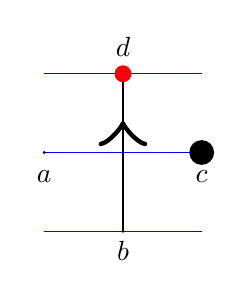
\begin{tikzpicture}[scale=1, transform shape]
\foreach \y in {0,1,2} \draw[blue] (-1,\y) -- (1,\y) ;
\foreach \x in {0} \foreach \y in {2} {\draw[>>] (\x,\y-2) -- (\x,\y) ;}
\draw [fill=black] (1,1) circle [radius=0.1] ;
\node[below] at (-1,0.9) {$a$}; {\draw (-1,1) circle [radius=0.01] ;}
\node[below] at (0,0) {$b$}; {\draw (0,0) circle [radius=0.01] ;}
\node[below] at (1,0.9) {$c$}; {\draw [fill=black] (1,1) circle [radius=0.15] ;}
\node[above] at (0,2.1) {$d$}; {\draw [red, fill=red] (0,2) circle [radius=0.1] ;}
\end{tikzpicture} &\scalebox{3}{$\rightsquigarrow$}&
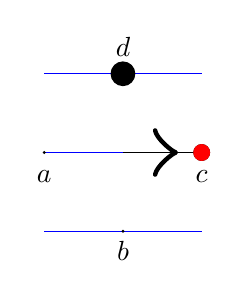
\begin{tikzpicture}[scale=1, transform shape]
\foreach \y in {0,1,2} \draw[blue] (-1,\y) -- (1,\y) ;
\foreach \x in {1} \foreach \y in {1} {\draw[>>] (\x-1,\y) -- (\x,\y) ;}
\draw [fill=black] (1,1) circle [radius=0.1] ;
\node[below] at (-1,0.9) {$a$}; {\draw (-1,1) circle [radius=0.01] ;}
\node[below] at (0,0) {$b$}; {\draw (0,0) circle [radius=0.01] ;}
\node[below] at (1,0.9) {$c$}; {\draw [red, fill=red] (1,1) circle [radius=0.1] ;}
\node[above] at (0,2.1) {$d$}; {\draw [fill=black] (0,2) circle [radius=0.15] ;}
\end{tikzpicture}
\end{tabular}
\end{center}
\caption{Elementary flip illustrating the relation $p(c)T(a,\mk b,\mk c;\mk d)\mk=p(d)T_r(d,\mk a,\mk b;\mk c)$.} \label{fig:flips1}
\end{figure}



%%A: la figure ci dessous pose un problème. La superposition des chiffres et des lettres est trop réduite dans la figure d'origine. C'est résolvable en mettant les scale à 0.7 et en rajoutant des espaces entre les tikspictures au niveau des right arrow.Mais le problème est l'alignement à gauche de l'ensemble : je l'ai donc désactivé le temps de trouver une solution si c'est possible... sinon j'ai fait une capture du résultat pour que l'ensemble soit centré par le biais d'une illustration...

%%\begin{figure}
%%\begin{center}
%%\begin{tabular}{m{4.1cm}m{0.5cm}m{4.1cm}m{0.5cm}m{4.1cm}}
%%\begin{tikzpicture}[scale=0.7]
%%\foreach \y in {0,1,2,3,4,5,6} \draw[blue] (-3,\y) -- (3,\y) ;

%%\foreach \x in {0} \foreach \y in {2,4,6} {\draw[>>] (\x,\y-2) -- (\x,\y) ;}
%%\foreach \x in {-1,1} \foreach \y in {3,5} {\draw[>>] (\x,\y-2) -- (\x,\y) ;}
%%\foreach \x in {-2,2} \foreach \y in {4} {\draw[>>] (\x,\y-2) -- (\x,\y) ;}

%%\node[below] at (0,0) {$a_{0,0}$};
%%\node[below] at (-1,1) {$a_{1,0}$};
%%\node[below] at (1,1) {$a_{0,1}$};
%%\node[below] at (-2,2) {$a_{2,0}$};
%%\node[below] at (0,2) {$a_{1,1}$};
%%\node[below] at (2,2) {$a_{0,2}$};
%%\node[below] at (-3,3) {$a_{3,0}$};
%%\node[below] at (-1,3) {$a_{2,1}$};
%%\node[below] at (1,3) {$a_{1,2}$};
%%\node[below] at (3,3) {$a_{0,3}$};
%%\node[below] at (-2,4) {$a_{3,1}$};
%%\node[below] at (0,4) {$a_{2,2}$};
%%\node[below] at (2,4) {$a_{1,3}$};
%%\node[below] at (-1,5) {$a_{3,2}$};
%%\node[below] at (1,5) {$a_{2,3}$};
%%\node[below] at (0,6) {$a_{3,3}$};

%%\foreach \x in {0} \foreach \y in {0} {\draw [red, fill=red] (\x,\y) circle [radius=0.1] ;}
%%\foreach \x in {-1,1} \foreach \y in {1} {\draw [red, fill=red] (\x,\y) circle [radius=0.1] ;}
%%\foreach \x in {-2,0,2} \foreach \y in {2} {\draw [red, fill=red] (\x,\y) circle [radius=0.1] ;}
%%\foreach \x in {-3,-1,1,3} \foreach \y in {3} {\draw [red, fill=red] (\x,\y) circle [radius=0.1] ;}
%%\foreach \x in {-2,0,2} \foreach \y in {4} {\draw [red, fill=red] (\x,\y) circle [radius=0.1] ;}
%%\foreach \x in {-1,1} \foreach \y in {5} {\draw [red, fill=red] (\x,\y) circle [radius=0.1] ;}
%%\foreach \x in {0} \foreach \y in {6} {\draw [red, fill=red] (\x,\y) circle [radius=0.1] ;}

%%\foreach \x in {0,1,2,3} {\draw [fill=black] (-\x,\x) circle [radius=0.15] ; \draw [fill=black] (\x,\x) circle [radius=0.15] ;}
%%\end{tikzpicture}\;\;\;\;
%%&\scalebox{1.5}{\quad$\rightsquigarrow$}&\quad
%%\begin{tikzpicture}[scale=0.7]
%%\foreach \y in {0,1,2,3,4,5,6} \draw[blue] (-3,\y) -- (3,\y) ;

%%\foreach \x in {1} \foreach \y in {1,3,5} {\draw[>>] (\x-2,\y) -- (\x,\y) ;}
%%\foreach \x in {2} \foreach \y in {2,4} {\draw[>>] (\x-2,\y) -- (\x,\y) ;}
%%\foreach \x in {3} \foreach \y in {3} {\draw[>>] (\x-2,\y) -- (\x,\y) ;}

%%\foreach \x in {-1} \foreach \y in {3,5} {\draw[>>] (\x,\y-2) -- (\x,\y) ;}
%%\foreach \x in {-2} \foreach \y in {4} {\draw[>>] (\x,\y-2) -- (\x,\y) ;}

%%\node[below] at (0,0) {$a_{0,0}$};
%%\node[below] at (-1,1) {$a_{1,0}$};
%%\node[below] at (1,1) {$a_{0,1}$};
%%\node[below] at (-2,2) {$a_{2,0}$};
%%\node[below] at (0,2) {$a_{1,1}$};
%%\node[below] at (2,2) {$a_{0,2}$};
%%\node[below] at (-3,3) {$a_{3,0}$};
%%\node[below] at (-1,3) {$a_{2,1}$};
%%\node[below] at (1,3) {$a_{1,2}$};
%%\node[below] at (3,3) {$a_{0,3}$};
%%\node[below] at (-2,4) {$a_{3,1}$};
%%\node[below] at (0,4) {$a_{2,2}$};
%%\node[below] at (2,4) {$a_{1,3}$};
%%\node[below] at (-1,5) {$a_{3,2}$};
%%\node[below] at (1,5) {$a_{2,3}$};
%%\node[below] at (0,6) {$a_{3,3}$};

%%\foreach \x in {0} \foreach \y in {0} {\draw [red, fill=red] (\x,\y) circle [radius=0.1] ;}
%%\foreach \x in {-1,1} \foreach \y in {1} {\draw [red, fill=red] (\x,\y) circle [radius=0.1] ;}
%%\foreach \x in {-2,0,2} \foreach \y in {2} {\draw [red, fill=red] (\x,\y) circle [radius=0.1] ;}
%%\foreach \x in {-3,-1,1,3} \foreach \y in {3} {\draw [red, fill=red] (\x,\y) circle [radius=0.1] ;}
%%\foreach \x in {-2,0,2} \foreach \y in {4} {\draw [red, fill=red] (\x,\y) circle [radius=0.1] ;}
%%\foreach \x in {-1,1} \foreach \y in {5} {\draw [red, fill=red] (\x,\y) circle [radius=0.1] ;}
%%\foreach \x in {0} \foreach \y in {6} {\draw [red, fill=red] (\x,\y) circle [radius=0.1] ;}

%%\foreach \x in {0,1,2,3} {\draw [fill=black] (-\x,\x) circle [radius=0.15] ; \draw [fill=black] (0,2*\x) circle [radius=0.15] ;}
%%\end{tikzpicture}
%%&  \scalebox{1.6}{\quad\;\;$\rightsquigarrow$} &\qquad
%%\begin{tikzpicture}[scale=0.7]
%%\foreach \y in {0,1,2,3,4,5,6} \draw[blue] (-3,\y) -- (3,\y) ;

%%\foreach \x in {0} \foreach \y in {2,4} {\draw[>>] (\x-2,\y) -- (\x,\y) ;}
%%\foreach \x in {1} \foreach \y in {1,3,5} {\draw[>>] (\x-2,\y) -- (\x,\y) ;}
%%\foreach \x in {-1} \foreach \y in {3} {\draw[>>] (\x-2,\y) -- (\x,\y) ;}
%%\foreach \x in {2} \foreach \y in {2,4} {\draw[>>] (\x-2,\y) -- (\x,\y) ;}
%%\foreach \x in {3} \foreach \y in {3} {\draw[>>] (\x-2,\y) -- (\x,\y) ;}

%%\node[below] at (0,0) {$a_{0,0}$};
%%\node[below] at (-1,1) {$a_{1,0}$};
%%\node[below] at (1,1) {$a_{0,1}$};
%%\node[below] at (-2,2) {$a_{2,0}$};
%%\node[below] at (0,2) {$a_{1,1}$};
%%\node[below] at (2,2) {$a_{0,2}$};
%%\node[below] at (-3,3) {$a_{3,0}$};
%%\node[below] at (-1,3) {$a_{2,1}$};
%%\node[below] at (1,3) {$a_{1,2}$};
%%\node[below] at (3,3) {$a_{0,3}$};
%%\node[below] at (-2,4) {$a_{3,1}$};
%%\node[below] at (0,4) {$a_{2,2}$};
%%\node[below] at (2,4) {$a_{1,3}$};
%%\node[below] at (-1,5) {$a_{3,2}$};
%%\node[below] at (1,5) {$a_{2,3}$};
%%\node[below] at (0,6) {$a_{3,3}$};

%%\foreach \x in {0} \foreach \y in {0} {\draw [red, fill=red] (\x,\y) circle [radius=0.1] ;}
%%\foreach \x in {-1,1} \foreach \y in {1} {\draw [red, fill=red] (\x,\y) circle [radius=0.1] ;}
%%\foreach \x in {-2,0,2} \foreach \y in {2} {\draw [red, fill=red] (\x,\y) circle [radius=0.1] ;}
%%\foreach \x in {-3,-1,1,3} \foreach \y in {3} {\draw [red, fill=red] (\x,\y) circle [radius=0.1] ;}
%%\foreach \x in {-2,0,2} \foreach \y in {4} {\draw [red, fill=red] (\x,\y) circle [radius=0.1] ;}
%%\foreach \x in {-1,1} \foreach \y in {5} {\draw [red, fill=red] (\x,\y) circle [radius=0.1] ;}
%%\foreach \x in {0} \foreach \y in {6} {\draw [red, fill=red] (\x,\y) circle [radius=0.1] ;}

%%\foreach \x in {0,1,2,3} {\draw [fill=black] (-\x,\x) circle [radius=0.15] ; \draw [fill=black] (-\x,6-\x) circle [radius=0.15] ;}
%%\end{tikzpicture}\\
%%\centering (a)&& \centering (b)&&\centering (c)
%%\end{tabular}
%%\end{center}
%%\caption{From $T$ to $T_r$ using flips.} \label{fig:flips2}
%%\end{figure}

\begin{figure}
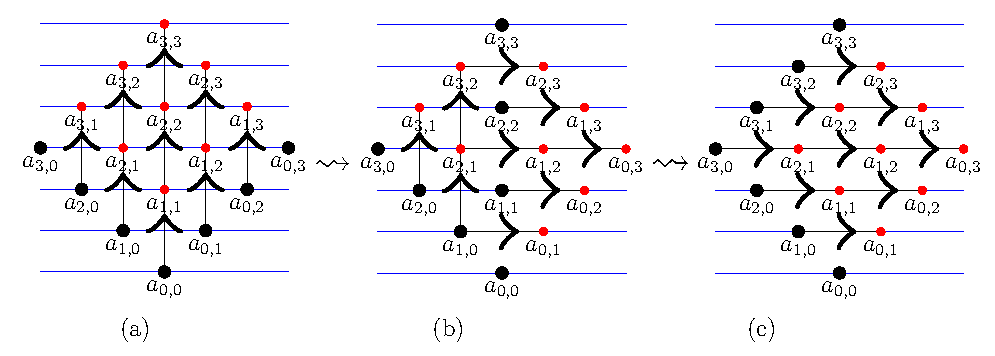
\includegraphics[scale=0.88]{Pictures/Figure-432.pdf} 
\caption{From $T$ to $T_r$ using flips.} \label{fig:flips2}
\end{figure}


Let us define the vertical lines: $V_{-1}=(x+(m-i)\vu+(m-i-1)\vv)_{0\leq i\leq m-1}$, $V_{0}=(x+(m-i)\vu+(m-i)\vv)_{0\leq i\leq m}$, $V_{1}=(x+(m-i-1)\vu+(m-i)\vv)_{0\leq i\leq m-1}$. From~\eqref{eq:tourne}, we deduce that:
\begin{align*}
\Pbb\big(\eta(V_1)\!=(a_{m,m-1},\ldots,a_{1,0}) \, \big| \; \eta(V_0)\!=(a_{m,m},\ldots,a_{0,0}), \eta(V_{-1})\!=(a_{m,m-1},\ldots,a_{1,0})\big)\\
=\prod_{i=0}^{m-1}T_r(a_{m-i,m},a_{m-i,m-i-1},a_{m-i-1,m-i-1};a_{m-i-1,m-i})
\end{align*}

Since this is true for any $x \in \Z_{e}^2$ and any $m\in\NN$, it follows that the rotation of $G(A,\pi_p)$, the space-time diagram of $A$, by the rotation $r$ is a space-time diagram of ${A}_r$, whose transition kernel is $T_r$, under one of its invariant measure that we denote by $\mu$ (observe that we do not specify the dependence on $A$ in that last notation, although the measure depends on $A$). Furthermore, we can express explicitly the finite-dimensional marginals of $\mu$. For any $m\in\NN$, we have
\begingroup
\allowdisplaybreaks
\begin{align}
\mu((&a_{i+1,i})_{0 \leq i \leq m-1},(a_{i,i})_{0 \leq i \leq m})\notag\\*
&\;=\Pbb\left(\eta(V_0)=(a_{m,m},\ldots,a_{0,0}), \eta(V_1)=(a_{m,m-1},\ldots,a_{1,0})\right)\notag\\*
&\; = \sum_{(a_{i,j}\, : \; i,i+1 \neq j)} \; \prod_{i=0}^m p(a_{i,0}) \prod_{j=1}^m p(a_{0,j}) \prod_{1\leq i,j\leq m} T(a_{i,j-1},a_{i-1,j-1},a_{i-1,j};a_{i,j}) \label{calcul_expl1}
\\*
\label{calcul_expl2}
&\; = \sum_{(a_{i,j}\, : \; {j<i})} \; \prod_{i=0}^m p(a_{i,0}) \prod_{j=1}^m p(a_{m,j}) \prod_{1\leq j\leq i+1\leq m} T_r(a_{i+1,j},a_{i+1,j-1},a_{i,j-1};a_{i,j})\mathrlap{\qed}
\end{align}
\endgroup
%\end{itemize}
\let\qed\relax
\end{proof}


Note that in Theorem~\ref{theo:referee} (case $g=r$), the reverse PCA is not necessarily an element of $\triang{S}{p}$. In the space-time diagram $G(A,\pi_p)$, the points $x,x+\vu,x+2\vu,\ldots,x+m\vu,x+m\vu+\vv,\ldots,x+m\vu+m\vv$ consist in independent random variables with distribution $p$. But if we now consider only the three points $x,x+\vv,x+\vu+\vv$, they have no reason to be independent, so that $\mu$ can be different from $\pi_p$. Proposition~\ref{theo:r-rev} below specifies the cases for which the reverse PCA $A_r$ is an element of $\triang{S}{p}$, meaning that $\mu=\pi_p$.

\begin{prop}\label{theo:r-rev}
Let $A \in \triang{S}{p}$. The following properties are equivalent:
\begin{enumerate}
\item \label{list4.4.1}$A$ is $\{r,r^{-1}\}$-quasi-reversible,
\item \label{list4.4.2}$A$ is $r$-quasi-reversible and $A_r \in \triang{S}{p}$,
\item \label{list4.4.3}$A$ is $r^{-1}$-quasi-reversible and $A_{r^{-1}} \in \triang{S}{p}$,
\item \label{list4.4.4}\Cond~\ref{cond:r1rev} and \Cond~\ref{cond:r3rev} hold,
\item \label{list4.4.5}$A$ is $D_4$-quasi-reversible.
\end{enumerate}
\end{prop}

\begin{proofc}
\begin{proof}[$\eqref{list4.4.1} \Rightarrow \eqref{list4.4.2}$] If $A$ is $r$-quasi-reversible, then the transition kernel $T_r$ of its $r$-reverse $A_r$ satisfies:
\[
\sum_{a\in S} p(a) T_r(d,a,b;c) = \sum_{a\in S} p(a)\frac{p(c)}{p(d)}T(a,b,c;d) = p(c),
\]
using \Cond~\ref{cond:r3rev}, since $A$ is $r^{-1}$-quasi-reversible. Thus, \Cond~\ref{cond-pm} holds for $T_r$ and, by Theorem~\ref{theo:gen0}, $A_r \in \triang{S}{p}$.
\let\qed\relax
\end{proof}
\begin{proof}[$\eqref{list4.4.1} \Leftarrow \eqref{list4.4.2}$] Since $A_r \in \triang{S}{p}$, by Corollary~\ref{cor:reversibility}, $A_r$ is $r^2$-quasi-reversible. Then, by the property~\eqref{list2.7.4}  of Proposition~\ref{prop:obvious}, $A$ is $r^3=r^{-1}$-quasi-reversible.
\let\qed\relax
\end{proof}
\begin{proof}[$\eqref{list4.4.1} \Leftrightarrow \eqref{list4.4.3}$] Same proof as $\eqref{list4.4.1} \Leftrightarrow \eqref{list4.4.2}$.
\let\qed\relax
\end{proof}
\begin{proof}[$\eqref{list4.4.1} \Leftrightarrow \eqref{list4.4.4}$] It is a consequence of Theorem~\ref{theo:referee}.
\let\qed\relax
\end{proof}
\begin{proof}[$\eqref{list4.4.1} \Leftrightarrow \eqref{list4.4.5}$] It is a consequence of the points $\eqref{list2.7.2}$ and $\eqref{list2.7.4}$ of Proposition~\ref{prop:obvious}, together with Corollary~\ref{cor:reversibility}.
\end{proof}
\let\qed\relax
\end{proofc}

\subsection{Independence properties of the space-time diagram} \label{sec:ind}

\begin{theo}\label{theo:iid_lines}
Let us consider a PCA $A \in \triangE{S}(p)$ and its stationary space-time diagram $G=(A,\pi_p)$. Then for any $|a|\leq 1$, the points of $G$ indexed by the discrete line $L_{a,b}=\{(x,y)\in \Z_{e}^2 \, : \; y=ax+b\}$ consist in i.i.d. random variables.
\end{theo}

\begin{proof}
This is a consequence of Proposition~\ref{prop:ind}. We can assume without loss of generality that $b=0$ and that $0< a \leq 1$, and we assume that the discrete line is non-empty. Let $(x,y)\in\Z_{e}^2$ be the first point with positive coordinates belonging to the integer line, so that we have in particular $0< y \leq x$. Let us define the sequence $(t_i)_{\in \Z}$ by $t_{i+kx}=i+ky$ for $i\in\{0,\ldots,y-1\}$ and $t_{i+kx}=y+\frac{(-1)^{i-y}-1}{2}+ky$ for $i\in\{y,\ldots,x-1\}$, and any $k\in\Z$. This sequence satisfies the conditions of Proposition~\ref{prop:ind}, so that $(\eta_{t_i}(i) : i\in\Z)\sim p^{\otimes \Z}$. Since $L_{a,b}\subset \{(i,t_i) : i\in \Z\}$, the result follows.
\end{proof}

\begin{theo}\label{theo:iid_lines2}
Let us consider a PCA $A\in \triangE{S}(p)$ satisfying \Cond~\ref{cond:r1rev} or \Cond~\ref{cond:r3rev}. Then, for any line of its stationary space-time diagram $G=(A,\pi_p)$, nodes on that line are i.i.d.
\end{theo}

\begin{proof}
We prove the result for a PCA $A\in \triangE{S}(p)$ satisfying \Cond~\ref{cond:r1rev}. In that case, $A$ is $r$-quasi-reversible. Now, take any line $L$ in $G$.

Let us now consider an equation of the form $y=ax+b$ with $|a|>1$, or $x=c$. We can assume without loss of generality that $b=0$. Let $(x,y) \in \Z_{e}^2$ be the first point with a positive coordinates belonging to the integer line, so that we have in particular $0<|x|<y$. Then we can perform flips, similarly as the ones done in the proof of the Theorem~\ref{theo:referee}, case $g=r$ (see Figure~\ref{fig:flips2}), to obtain that, for any $m$, the points $m\vu, (m-1)\vu, \ldots, \vu, (0,0), (x,y), (2x,2y), \dots, (kx,ky)$ (with $k = \lfloor m/(x+y) \rfloor$) are i.i.d. In particular, $(0,0), (x,y), (2x,2y), \dots, (kx,ky)$ are i.i.d.
\end{proof}

\subsubsection*{PCA with strong independence}
Let us recall the notations $\vu= (-1,1)$, $\vv = (1,1)$.

\begin{defi}\label{def:lrind}
Let $G=(A,\mu)$ be a stationary space-time diagram of a PCA $A$ under one of its invariant measure $\mu$. We say that $G$ is \emph{top} (resp. \emph{bottom}, \emph{left}, \emph{right}) \emph{i.i.d.} if, for any $x \in \Z_{e}^2$, $\{\eta(x), \eta(x-\vu),\eta(x-\vv)\}$ (resp.$\{\eta(x),\eta(x+\vu), \eta(x+\vv)\}$, $\{\eta(x),\eta(x-\vu),\eta(x+\vv)\}$ $\{\eta(x),\eta(x+\vu),\eta(x-\vv)\}$) are i.i.d. A PCA is said to be 3-to-3 i.i.d. if it is top, bottom, left and right i.i.d.
\end{defi}

\begin{prop}
$G=(A,\mu)$ is both top and bottom i.i.d. if and only if $A \in \triangE{S}$ and $\mu$ is its invariant HZPM.
\end{prop}

\begin{proof}
Let $G=(A,\mu)$ be a top and bottom i.i.d. PCA. We denote by $p$ the one-dimensional marginal of $\mu$. Then, we have, for any $a,b,c,d \in S$,
\begin{align*}
\Pbb\left(\eta(x)=d,\eta(x-\vu)=a,\eta(x-\vv)=c\right) & = p(a) p(d) p(c) \text{ (top i.i.d.)} \\
& =\!\sum_{b\in S} p(a) p(b) p(c) T(a,b,c;d)\!\!\text{ (bottom i.i.d.)}.
\end{align*}
Hence, \Cond~\ref{cond-pm} holds and, by Theorem~\ref{theo:gen0}, $A \in \triang{S}{p}$, and $\mu=\pi_p$. The reverse statement is trivial.
\end{proof}

\begin{prop}
$G=(A,\mu)$ is 3-to-3 i.i.d. if and only if $A$ is a $D_4$-quasi-reversible PCA of $\triangE{S}$ and $\mu$ is its invariant HZPM.
\end{prop}

\begin{proof}
Let $(A,\mu)$ be a 3-to-3 i.i.d. PCA, then $A \in \triangE{S}$ because $A$ is both top and bottom i.i.d. Moreover,
\begin{align*}
p(a)p(b)p(d) & = \sum_{c\in S} p(a)p(b)p(c) T(a,b,c;d) \\
\text{ and } \quad p(c)p(b)p(d) & = \sum_{a\in S} p(a)p(b)p(c) T(a,b,c;d),
\end{align*}
using the fact that $A$ is top and left (resp. right) i.i.d. But these are respectively \Cond~\ref{cond:r1rev} and \Cond~\ref{cond:r3rev} and, so, by Theorem~\ref{theo:r-rev}, $A$ is $D_4$-quasi-reversible. The reverse statement is trivial.
\end{proof}

Note that $G=(A,\mu)$ is top, bottom, and left (resp. right) i.i.d. if and only if $A$ is a $r$-quasi-reversible PCA (resp. $r^{-1}$-quasi-reversible PCA) of $\triangE{S}$ and $\mu$ is its invariant HZPM.

\subsubsection*{Connection with previous results for PCA with memory one}
In the special case when the PCA has memory one, meaning that the transition probabilities $T(a,b,c;d)$ do no depend on $b\in S$, \Cond~\ref{cond-pm} reduces to: $\forall a,c,d\in S$, $p(d)=T(a,\cdot\,, c ; d).$ So, the only PCA having an invariant HZPM are trivial ones (no time dependence at all). In that context, it is in fact more relevant to study PCA having simply an invariant horizontal product measure, as done in~\cite{mm_ihp}. Observe that when there is no dependence on $b\in S$, \Cond~\ref{cond:r1rev} et \Cond~\ref{cond:r3rev} become
\[
\forall a,d \in S,\ \sum_{c \in S} p(c) T(a,\cdot,c;d) = p(d) \ \text{and} \ \forall c,d \in S,\ \sum_{a \in S} p(a) T(a,\cdot\,,c;d) = p(d).
\]
We recover the two sufficient conditions for having an horizontal product measure, as described in Theorem~5.6 of~\cite{mm_ihp}. In that article, the space-time diagrams are represented on a regular triangular lattice, which is more adapted to the models that are considered. The authors show that under one or the other of these two conditions, there exists a transversal PCA, so that after an appropriate rotation of the triangular lattice, the stationary space-time diagram can also be described as the one of another PCA. With our terminology, this corresponds to a quasi-reversibility~property.

\subsection{PCA with an explicit invariant law that is not HZPM}\label{notHZPM}

As already mentioned, if a PCA $A \in \triang{S}{p}$ satisfies \Cond~\ref{cond:r1rev} and not \Cond~\ref{cond:r3rev} (or the reverse), we get a PCA $C=A_r$ (or $A_{r^{-1}}$) for which we can compute exactly the marginals of an invariant measure $\mu$, see equations~\eqref{calcul_expl1} and~\eqref{calcul_expl2}. Using the previous results, we can describe conditions on the transitions of a PCA $C$ for being of the form $C=A_r$, with $A$ having an invariant $p$-HZMP. We thus obtain next corollary, highlighting a family of PCA having an invariant measure that can be computed explicitly, although it does not have a well-identified form.

\begin{coro}\label{theo:cool}
Let $C$ be a PCA with transition kernel $U$. If there exists a probability distribution $p$ such that \Cond~\ref{cond:r1rev} and \Cond~\ref{cond:r3rev} hold, then there exists a unique probability distribution $\mu$ on $S^{\ZZ_0} \times S^{\ZZ_{1}}$ such that
\begin{itemize}
\item $\mu$ is invariant by $C$,
\item $(C,\mu)$ is $\{r^{-1},r\}$-quasi-reversible and
\begin{itemize}
\item its $r^{-1}$-reverse is $(C_{r^{-1}},\pi_p)$ with $C_{r^{-1}} \in \triang{S}{p}$, and the transition kernel of $C_{r^{-1}}$ is equal to $U_{r^{-1}}$.
\item its $r$-reverse is $(C_{r},\pi_p)$ with $C_{r} \in \triang{S}{p}$, and the transition kernel of $C_r$ is equal to $U_r$.
\end{itemize}
\item $\mu_{|\ZZ_0} = p^{\otimes \ZZ_0}$ and $\mu_{|\ZZ_{1}} = p^{\otimes \ZZ_{1}}$.
\end{itemize}
Moreover, we have explicit formulas for marginals of $\mu$.
\end{coro}

In Section~\ref{sec:binary}, Example~\ref{exemple:binaire} provides an example of a PCA satisfying only \Cond~\ref{cond:r1rev}, so that its $r$-reverse $A_r$ satisfies the conditions of Corollary~\ref{theo:cool} above.

\section{Horizontal zigzag Markov chains}\label{sec:markov}

After having extensively studied PCA with memory two having an invariant measure with a product form, we now focus on PCA having an invariant measure with a Markovian form, with a similar approach. We characterize such PCA, and among them, those having a quasi-reversibility property, thus justifying the results that were announced in Table~\ref{table:pres-HZMC}. As in the previous section, our results will also allow us to exhibit a new family of PCA having an invariant measure that can be computed explicitly, although it does not have a simple form.

\subsection{Conditions for having an invariant HZMC} \label{sec:invHZMC}

In this section, we recall some previous results obtained in~\cite{Casse17} about PCA with memory two having an invariant measure which is a Horizontal Zigzag Markov Chain. Our purpose is to keep the present article as self-contained as possible.

First, let us recall what is a $(F,B)$-HZMC distribution. This is the same notion as $(D,U)$-HZMC in~\cite{Casse17}, but to be consistent with the orientation chosen here for the space-time diagrams, we prefer using the notations $F$ for forward in time, and $B$ for backward in time (rather than $D$ for down and $U$ for up). The definition we give below relies on the following Lemma~\ref{lemm5.1}.

\begin{lemm}\label{lemm5.1}
Let $S$ be a finite set, and let $F = (F(a;b) : a,b \in S)$ and $B = (B(b;c) : b,c \in S)$ be two positive transition matrices from $S$ to $S$. We denote by $\rho_B$ (resp. $\rho_F$) the invariant probability distribution of $B$ (resp. $F$), that is, the normalised left-eigenvector of $B$ (resp. $F$) associated to the eigenvalue~$1$. If $FB=BF,$ then $\rho_B=\rho_F$.
\end{lemm}

\begin{proof}
Note that by Perron--Frobenius, $B$ and $F$ have a unique invariant probability distribution, satisfying respectively $\rho_BB=B$ and $\rho_F F=F$. Since $FB=BF$, we have $ \rho_B FB = \rho_B B F = \rho_B F,$ so that the vector $\rho_B F$ is an invariant probability distribution of $B$. By uniqueness, we obtain $\rho_B F = \rho_B$. Since the invariant probability distribution of $F$ is also unique, we obtain $\rho_B=\rho_F$.
\end{proof}

\begin{defi}\label{def:hzmc}
Let $S$ be a finite set, and let $F$ and $B$ be two transition matrices from $S$ to $S$, such that $FB=BF$. We denote by $\rho$ their (common) left-eigenvector associated to the eigenvalue~$1$. The $(F,B)$-HZMC (for \emph{Horizontal Zigzag Markov Chain}) on $S^{\ZZ_{t}} \times S^{\ZZ_{t+1}}$ is the distribution $\zeta_{F,B}$ such that, for any $n \in \ZZ_t$, for any $a_{-n},a_{-n+2},\ldots,a_n \in S, b_{-n+1},n_{n+3},\ldots,b_{n-1} \in S$,
\begin{multline*}
\Pbb\left((\zeta_{F,B}(i,t)= a_i, \zeta_{F,B}(i,t+1) = b_i :-n\leq i\leq n)\right) \\
 = \rho(a_{-n}) \prod_{i=-n+1}^{n-1} F(a_{i-1};b_i) B(b_i;a_{i+1}).
\end{multline*}
\end{defi}

\begin{figure}
\begin{center}
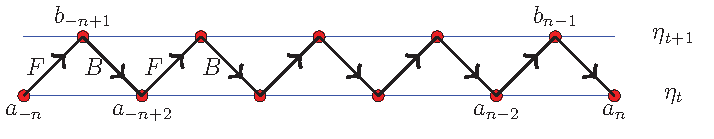
\includegraphics[scale=1]{Pictures/Figure_51.pdf} 
%%\begin{tikzpicture}
%%\foreach \y in {1,2} \draw[blue] (-5,\y) -- (5,\y) ;
%%\foreach \x in {-4,-2,\dots,4} \foreach \y in {2} {\draw [fill=red] (\x,\y) circle [radius=0.1] ;}
%%\foreach \x in {-5,-3,\dots,5} \foreach \y in {1} {\draw [fill=red] (\x,\y) circle [radius=0.1] ;}
%%\foreach \x in {-4,-2,\dots,4} \foreach \y in {2} {\draw[->-,thick] (\x,\y) -- (\x+1,\y-1) ;}
%%\foreach \x in {-4,-2,\dots,4} \foreach \y in {2} {\draw[->-,thick] (\x-1,\y-1) -- (\x,\y) ;}
%%\node at (6,2) {$\eta_{t+1}$};
%%\node at (6,1) {$\eta_{t}$};

%%\node[below] at (-5,1) {$a_{-n}$};
%%\node[below] at (-3,1) {$a_{-n+2}$};
%%\node[below] at (3,1) {$a_{n-2}$};
%%\node[below] at (5,1) {$a_{n}$};
%%\node[above] at (-4,2) {$b_{-n+1}$};
%%\node[above] at (4,2) {$b_{n-1}$};

%%\node[left] at (-4.5,1.5) {$F$};
%%\node[left] at (-3.5,1.5) {$B$};
%%\node[left] at (-2.5,1.5) {$F$};
%%\node[left] at (-1.5,1.5) {$B$};
%%\end{tikzpicture}
\end{center}
\caption{Illustration of Definition~\ref{def:hzmc}.}
\end{figure}

We give a simple necessary and sufficient condition that depends on both $T$ and $(F,B)$ for a $(F,B)$-HZMC to be an invariant measure of a PCA with transition kernel $T$ (in order to remove any ambiguity, let us precise that the definition of a transition kernel is exactly the same as in the previous sections).

\begin{prop}[Lemma~5.10 of~\cite{Casse17}] \label{prop:Casse17}
Let $S$ be a finite set. Let $A$ be a PCA with positive rates and let $F$ and $B$ be two transition matrices from $S$ to $S$. The $(F,B)$-HZMC distribution is an invariant probability distribution of $A$ if and only if:\\
\Cond~\ref{cond:DU-HZMC}: for any $a,c,d \in S$, $F(a;d)B(d;c) = \sum_{b \in S} B(a;b)F(b;c) T(a,b,c;d).$
\end{prop}

We denote by $\triang{S}{F,B}$ the subset of positive-rates PCA with set of symbols $S$ having an invariant $(F,B)$-HZMC.

In the context of PCA having an invariant $(F,B)$-HZMC, Proposition~\ref{prop:ind} can be extended as follows. The proof being similar, we omit it.
%\pagebreak


\begin{prop}\label{prop:ind_m}
Let $A\in\triang{S}{F,B}$, of stationary space-time diagram $G(A,\linebreak\zeta_{F,B})=(\eta_t(i) : t \in \ZZ, i \in \ZZ_t)$. For any zigzag polyline $(i,t_i)_{m\leq i\leq n}$, and any $(a_i)_{m \leq i \leq n}\in S^{n+1}$, we have
\begin{align*}
\Pbb\left(\eta(i,t_i) = a_i : m \leq i \leq n\right) = \rho(a_0) \mathop{\prod_{m\in\{0,\ldots,n-1\}}}_{t_{i+1}=t_i+1} F(a_i;a_{i+1}) \mathop{\prod_{m\in\{0,\ldots,n-1\}}}_{t_{i+1}=t_i-1} B(a_i;a_{i+1}).
\end{align*}
\end{prop}

In general, the knowledge of the transition kernel $T$ alone is not sufficient to be able to tell if the PCA $A$ admits or not an invariant $(F,B)$-HZMC. Until now, the characterization of PCA having an invariant $(F,B)$-HZMC is known in only two cases: when $|S|=2$~\cite[Theorem~5.3]{Casse17}, and when $F=B$~\cite[Theorem~5.2]{Casse17}. In the other cases ($F \neq B$ and $|S|>2$), it is an open problem.

\subsection{Quasi-reversible PCA with invariant HZMC}

This section is devoted to PCA having an HZMC invariant measure, and that are (quasi-)reversible.

Let $A\in \triang{S}{F,B}$. For $a,b\in S$, let us define
\[
\Bh (b;a) = \frac{\rho(a)}{\rho(b)} B(a;b) \text{ and } \Fh (b;a) = \frac{\rho(a)}{\rho(b)} F(a;b).
\]

We also introduce the notations $M_{-\vu}=B$ and $M_{\vv}=F$ (recall that $\vu=(-1,1)$ and $\vv=(1,1)$). For $g\in D_4$, we define
\[
p_{FB}(g(a,b,c))\isdef \rho(g(a))M_{g(-\vu)}(g(a),g(b))\,M_{g(\vv)}(g(b),g(c)),
\]
where $g(-\vu)$ corresponds to the vector $g(a)g(b)$, and $g(\vv)$ to $g(b)g(c)$ (note again the small abuse of notation for the images of the vertices by the permutation induced by $g$). If $g$ is the identity, we have $p_{FB}(a,b,c)=\rho(a)B(a,b)F(b,c).$ And for example in the case where $g=r$, we have
\[
p_{FB}(r(a,b,c))=p_{FB}(d,a,b)=\rho(d)M_{-\vv}(d,a)B(a,b)=\rho(a)F(a,b)B(a,b).
\]

From the transition kernel $T$ of $A$, we define a map $T_g: S^3 \times S\to \mathbb R_+$ by:
\[
\forall a,b,c,d\in S, \quad T_g(g(a,b,c);g(d))\isdef\frac{p_{FB}(a,b,c)}{p_{FB}(g(a,b,c))}T(a,b,c;d).
\]

For example, in the case where $g=r$, this gives:
\begin{equation}\label{eq:rrevtm}
\forall a,b,c,d\in S, \quad T_r(d,a,b;c)\isdef \frac{F(b;c)}{F(a;d)} T(a,b,c;d).
\end{equation}
The expressions of $T_{r^2}, T_{h},$ and $T_{r^{-1}}$ can be found in Table~\ref{table:pres-HZMC}.

Observe that $T_g$ is not necessarily a transition kernel. For example, $T_r$ is a transition kernel if and only if:
\[
\forall a,c,d \in S, \quad \sum_{c\in S} \frac{F(b;c)}{F(a;d)} T(a,b,c;d)=1,
\]
which is equivalent to \Cond~\ref{cond:r1DU}, see again Table~\ref{table:pres-HZMC}. Analogously, $T_{r^{-1}}$ is a transition kernel if and only if \Cond~\ref{cond:r3DU} is satisfied. And it appears that as soon as a PCA belongs to $\triang{S}{F,B}$, $T_{r^2}$ and $T_h$ are transition kernels, since \Cond~\ref{cond:DU-HZMC} is satisfied.

\begin{theo}\label{theo:refereeHZMC}
A PCA $A \in \triang{S}{F,B}$ of transition kernel $T$ is $g$-quasi-reversible if and only if $T_g$ is a transition kernel. In that case, $T_g$ is the transition kernel of the $g$-reverse $A_g$ of $A$.
\end{theo}

The next result is a direct consequence of Theorem~\ref{theo:refereeHZMC}.

\begin{coro}\label{cor:reversibilityHZMC}
Any PCA $A \in \triang{S}{F,B}$ is $r^2$-quasi-reversible and $h$-quasi-reversible.
\end{coro}

\begin{proof}[Proof of Theorem~\ref{theo:refereeHZMC}] The cases $g=\id$ and $g=v$ are obvious by Proposition~\ref{prop:obvious}, and the cases $g=h$ and $g=r^2$ can be handled exactly as in the proof of Theorem~\ref{theo:referee}.
We thus focus on the case $g=r$, for which the proof also follows the same idea as in Theorem~\ref{theo:referee}.
%\begin{itemize}
%\item[$\bullet$]
Suppose that $A$ is $r$-quasi-reversible, and denote by $\tT$ the transition kernel of $A_r$. Then, for any $a,b,c,d\in S$, and any $x \in \Z_{e}^2$,
\begin{equation}\label{eq-rev-mark}
\begin{aligned}
\tT(d,a,b;c)= \Pbb\left(\eta(x+\vv)=c | \eta(x+\vu+\vv)=d,\eta(x+\vu)=a,\eta(x)=b\right)\\
= \frac{\rho(a) B(a;b) F(b;c) T(a,b,c;d)}{\sum_{c'\in S} \rho(a) B(a;b) F(b;c') T(a,b,c';d)} = \frac{F(b;c) T(a,b,c;d)}{\sum_{c'\in S} F(b;c') T(a,b,c';d)}.
\end{aligned}
\end{equation}

For some $x \in \Z_{e}^2$, let us reintroduce the pattern $L=(x,x+\vu,x+\vv, x+2\vu,\linebreak x+\vu+\vv,x+2\vu+\vv)$, see Figure~\ref{fig:pattern}. For $a_0,b_0,b_1,c_0,c_1,d_0 \in S$, we are interested in the quantity: $Q(a_0,b_0,b_1,c_0,c_1,d_0)=\Pbb\left(\eta(L)=(a_0,b_0,b_1,c_0,c_1,d_0)\right).$

On the one hand, we have
\begin{multline*}
Q(a_0,b_0,b_1,c_0,c_1,d_0)\\
=\rho(c_0) B(c_0;b_0) B(b_0;a_0) F(a_0;b_1) T(b_0,a_0,b_1;c_1) T(c_0,b_0,c_1;d_0).
\end{multline*}
On the other hand, we have
\[
Q(a_0,b_0,b_1,c_0,c_1,d_0)=\sum_{b'_1,c'_1\in S}Q(a_0,b_0,b'_1,c_0,c'_1,d_0)\tT(d_0,c_0,b_0;c_1)\tT(c_1,b_0,a_0;b_1).
\]

Using the expressions of $\tT(d_0,c_0,b_0;c_1)$ and $\tT(c_1,b_0,a_0;b_1)$ given by~\eqref{eq-rev-mark} and simplifying, we get:
\begin{multline*}
\bigg(\sum_{b\in S} F(a_0;b) T(b_0,a_0,b;c_1) \bigg) \bigg(\sum_{c\in S} F(b_0;c) T(c_0,b_0,c;d_0) \bigg)\\
= F(b_0;c_1) \sum_{b,c\in S} F(a_0;b) T(b_0,a_0,b;c) T(c_0,b_0,c;d_0).
\end{multline*}
Now summing on $d_0 \in S$, we find, for any $b_0,c_1\in S$,
\[
F(b_0;c_1) = \sum_{b\in S} F(a_0;b) T(b_0,a_0,b;c_1),
\]
so that $\tT=T_r$.

%\item[$\bullet$]
Conversely, suppose that $A$ is a PCA having an invariant measures $(F,B)$-HZMC and that~\Cond~\ref{cond:r1DU} holds. Then, we can perform flips thanks to~\eqref{eq:rrevtm} as in Figures~\ref{fig:flips1} and~\ref{fig:flips2} to obtain the result.
%\qedhere
%\end{itemize}
\end{proof}

\subsection{PCA with an explicit invariant law that is not HZMC}\label{sec:notmarkov}

As mentioned in Section~\ref{notHZPM}, there exist PCA $A\in\triangE{S}(p)$ that are $r$-quasi-reversible, and for which the $r$-reverse $A_r$ does not belong to $\triangE{S}(p)$. In that case, $A_r$ has an invariant measure $\mu$ which is not a product measure, and for which we know formulas allowing to compute exactly all the marginals, see equations~\eqref{calcul_expl1} and~\eqref{calcul_expl2}. Let us point out that the measure $\mu$ cannot be a $(F,B)$-HZMC. Indeed, consider the stationary space-time diagram $(A,\pi_p)=(\eta(i,t): (i,t) \in \Z_{e}^2)$, and assume that $\mu$ is a $(F,B)$-HZMC measure. Then, the marginal of size one of $\mu$ is equal to $\rho=p$, and for any $x\in \Z_{e}^2$, we have $\Pbb\left(\eta(x+\vu)=a,\eta(x)=b\right)=p(a)p(b)=\rho(a)F(a;b)$ and $\Pbb\left(\eta(x)=b,\eta(x+\vv)=c\right)=p(b)p(c)=\rho(c)B(c;b)$. Thus, we obtain \linebreak$F(a;b)=B(c;b)=p(b)$ for any $a,b,c\in S$, meaning that the $(F,B)$-HZMC is in fact a $p$-HZMP, which is not possible since $A_r$ does not belong to $\triangE{S}(p)$.

So, the PCA $A_r$ has an invariant measure that we can compute, and that has neither a product form nor a Markovian one. That was a real surprise of this work. We give an explicit example of such a PCA in Section~\ref{sec:binary}, see Example~\ref{exemple:binaire}.

Similarly, if a PCA $A$ with a $(F,B)$-invariant HZMC is $r$-quasi-reversible, and is such that its $r$-reverse $A_r$ does not have an invariant HZMC, then we can compute exactly the invariant measure of $A_r$, although it does not have a well-known form. This provides an analogous of Corollary~\ref{theo:cool}, in the Markovian case. Precisely, next Corollary~\ref{theo:cool_hzmc} gives conditions on the transitions of a PCA $C$ for being of the form $C=A_r$, with $A$ having a $(F,B)$-invariant HZMC. To the best knowledge of the authors, this is the first time that we can compute from the transition kernel an invariant law that is not Markovian.

\begin{coro}\label{theo:cool_hzmc}
Let $C$ be a PCA of positive transition kernel $U$. If there exist two positive transition matrices $F$ and $B$ from $S$ to $S$ such that $FB=BF$, and such that the two following conditions hold:

\begin{cond} \label{cond:eqrDU-D}
for any $a,b,c \in S$, $F(b;c) = \sum_{d\in S} F(a;d) U(d,a,b;c)$;
\end{cond}

\begin{cond} \label{cond:eqrDU-U}
for any $a,c,d \in S$, $B(d;c) = \sum_{b\in S} B(a;b) U(d,a,b;c)$;
\end{cond}

\noindent% exceptionnellement justifié
then there exists a probability measure $\mu$ on $S$ such that
\begin{itemize}
\item $\mu$ is invariant by $C$,
\item $(C,\mu)$ is $\{r,r^{-1}\}$-quasi-reversible and
\begin{itemize}
\item its $r^{-1}$-reverse is $(C_{r^{-1}},\zeta_{F,B})$, with $C_{r^{-1}}\in\triang{S}{F,B}$, and the transition kernel of $C_{r^{-1}}$ is given by $T(a,b,c;d) = \frac{F(a;d)}{F(b;c)} U(d,a,b;c)$.
\item its $r$-reverse is $(C_r,\zeta_{\Bh,\Fh})$, with $C_r\in\triang{S}{\Bh,\Fh}$, and the transition kernel of $C_{r}$ is given by $T_{r^2}(c,d,a;b) = \frac{B(a;b)}{B(d;c)} U(d,a,b;c)$.
\end{itemize}
\end{itemize}

Moreover, we have explicit formulas for marginals of $\mu$.
\end{coro}

Note that in the above Theorem~\ref{theo:refereeHZMC}, the transition kernel $T$, which is the transition kernel of $C_{r^{-1}}$, corresponds to the transition kernel of the PCA $A$ (having a $(F,B)$-invariant HZMC) such that $C=A_r$. The transition kernels $T$ of $C_{r^{-1}}$ and $T_{r^2}$ of $C_r$ can be written as being equal respectively to $U_{r^{-1}}$ and $U_r$, but with $(F,B)$ replaced by $(B,M_{-\vv})$ when applying the formulas given in Table~\ref{table:pres-HZMC}.

\begin{rema}
In \Cond~\ref{cond:eqrDU-D} (resp. \Cond~\ref{cond:eqrDU-U}), by putting $a=b$ (resp. $a=d$), we find that for any $a\in S$, the vector $(F(a;d) : d \in S) $ (resp. $(B(a;b) : b \in S)$) is the left eigenvector of $(U(d,a,a;c))_{d,c \in S}$ (resp. $(U(a,a,b;c))_{b,c \in S}$) associated to the eigenvalue~$1$. In particular, this allows to determine $F$ and $B$, knowing only $U$. This is in contrast with Proposition~\ref{prop:Casse17}, where in general, the knowledge of $T$ does not allow to find $F$ and $B$.
\end{rema}


\begin{proof}
Let us define
\[
T(a,b,c;d) = \frac{F(a;d)}{F(b;c)}U(d,a,b;c).
\]

\goodbreak
Then, as \Cond~\ref{cond:eqrDU-D} and \Cond~\ref{cond:eqrDU-U} hold, we can check that $T$ is a transition kernel and satisfies \Cond~\ref{cond:DU-HZMC}, so $\zeta_{F,B}$ is an invariant measure of the PCA whose transition kernel is $T$. Moreover,
\[
\sum_{c\in S} F(b;c) {T}(a,b,c;d) = \sum_{c\in S} F(a;d) U(d,a,b;c) = F(a;d).
\]
That is \Cond~\ref{cond:r1DU}, and we conclude by application of Theorem~\ref{theo:refereeHZMC} (case $g=r$). Finally, multidimensional laws of $\mu$ are deduced from the space-time diagram $(C,\mu)$. Indeed, after action of the rotation $r^{-1}$, it has the same distribution as $(C_{r^{-1}},\zeta_{F,B})$ whose transition kernel is $T$. So, we can compute all the finite-dimensional marginals of the space-time diagram, and in particular the multidimensional laws of $\mu$.
\end{proof}

\section{Applications to statistical physics}\label{sec:sp}

In many models of statistical physics (6 and 8-vertex models, enumeration of directed animals, TASEP model, First Passage Percolation / Last Passage Percolation, Eden growth model, Box-Ball Systems\dots), one can find a PCA of order 1 or 2 that provides an alternative description of the system. In most cases, the original models are integrable only on a submanifold of their parameter space, and this corresponds to choices of parameters for which the corresponding PCA has a simple invariant measure, with a product or a Markovian structure.

In Section~\ref{sec:8V} and~\ref{sec:animals}, we show that using this PCA approach, results of previous sections provide new proofs of known results about the 8-vertex model and about the enumeration of directed animals, after associating suitable PCA with these two models. This gives a simpler alternative to transfer-matrix methods, that does not require tedious computations.

The PCA approach also often suggests relevant ways to extend the initial models of statistical physics. Let us indeed assume that when studying the PCA involved, it appears that the family of parameters for which they have a closed-form invariant measure belong to a larger submanifold, defined with more parameters. Then, one can try to backtrack this observation to the original model, by the introduction of new parameters preserving the physical meaning of the model, with a larger domain of parameters on which the model is integrable. This is what we illustrate in Section~\ref{sec:TASEP}, where we define a new TASEP model with variable speed that extends the classical parallel TASEP. The results of previous sections (Theorem~\ref{theo:gen0} and~Proposition~\ref{prop:Casse17}) do not apply directly because the PCA does not have positive rates. Nevertheless, our techniques can still be used to compute some invariant measures of this new model.

\subsection{The \texorpdfstring{$8$}{8}-vertex model} \label{sec:8V}

For some $k\in 2\Z$, we consider the graph $G_k$ whose set of vertices is $V_k=\Z_{e}^2 \cap [-k,k]^2$, the restriction of the even lattice to a finite box, and whose set of edges is $E_k=\{(x,x+\vu) : x,x+\vu\in V_k\}\cup\{(x,x+\vv) : x,x+\vv\in V_k\}$. We define the boundary of $V_k$ by $\partial V_k=\{(x_1,x_2)\in V_k : \max(|x_1|,|x_2|)=k\}$.

For each edge of $G_k$, we choose an orientation. This defines an orientation $O$ of $G_k$, and we denote by $O_k$ the set of orientations of $G_k$. For a given orientation $O\in O_k$, and an edge $e \in E_k$, we denote:
\[
o(e) =
\begin{cases}
0 & \text{if the edge $e$ is oriented from top to bottom in $O$ ($\searrow$ or $\swarrow$)},\\
1 & \text{if the edge $e$ is oriented from bottom to top in $O$ ($\nwarrow$ or $\nearrow$)}.
\end{cases}
\]
Hence, an orientation $O\in O_k$ can be seen as an element $(o(e))_{e \in E_k}$ of $\{0,1\}^{E_k}$.

Around each vertex $x\in V_k\setminus \partial V_k$, there are 4 oriented edges, giving a total of 16 possible local configurations, defining the \emph{type} of the vertex $x$. In the 8-vertex model case, we consider only the orientations $O$ such that around each vertex $x\in V_k\setminus \partial V_k$, there is an even number ($0$, $2$ or $4$) of incoming edges, so that only $8$ local configurations remain, see Figure~\ref{fig:8v}. To each local configuration $i$ among these 8 local configurations, we associate a local weight $w_i>0$. This allows to define a global weight $W$ on the set $\tilde O_k$ of admissible orientations, by:
\begin{equation*}
W(O) = \prod_{x\in V_k\setminus \partial V_k} w_{\text{type}(x)}, \quad \text{ for } O\in\tilde O_k.
\end{equation*}
Thanks to these weights, we finally define a probability distribution $\mathbb{P}_W$ on $\tilde O_k$, by:
\begin{equation*}
\pw{O} = \frac{W(O)}{Z_k}, \qquad \text{ with } \quad {Z_k=\sum_{O \in \tilde O_k} W(O)}.
\end{equation*}

\begin{figure}
\begin{center}
\begin{tabular}{c|c|c|c}
$w_1=w_2=a$ & $w_3=w_4=b$ & $w_5=w_6=c$ & $w_7=w_8=d$ \\ \hline
\espace \haut{1} 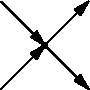
\includegraphics[scale=0.5]{Pictures/typeb1}&
\haut{3}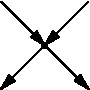
\includegraphics[scale=0.5]{Pictures/typeb3} &
\haut{5}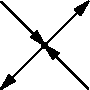
\includegraphics[scale=0.5]{Pictures/typeb5} &
\haut{7} 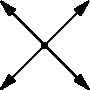
\includegraphics[scale=0.5]{Pictures/typeb7} \\
\haut{2} 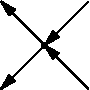
\includegraphics[scale=0.5]{Pictures/typeb2} &
\haut{4} 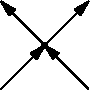
\includegraphics[scale=0.5]{Pictures/typeb4} &
\haut{6}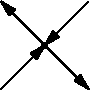
\includegraphics[scale=0.5]{Pictures/typeb6} &
\haut{8}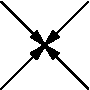
\includegraphics[scale=0.5]{Pictures/typeb8} 
\end{tabular}
\end{center}
\caption{The 8 possible local configurations around any vertex.}\label{fig:8v}
\end{figure}

In the following, we assume that the parameters satisfy $w_1=w_2=a$, $w_3=w_4=b$, $w_5=w_6=c$ and $w_7=w_8=d$, which corresponds to the most studied 8-vertex model. We furthermore assume that $a+c=b+d$. Let us briefly comment on this condition. Among $6$ and $8$-vertex models, a different case that has attracted much attention is the case when $a=b$, which corresponds to the \emph{XXZ model}~\cite{DGHMT16}. But from a physical point of view, this condition is quite restrictive, since it amounts to assuming that the oxygen atoms are arranged on a square lattice. We can relax this condition by assuming that the oxygen atoms are arranged on a diamond-shaped lattice, and within this framework, an interesting specific case for some ranges of temperature and pressure consists in assuming that $a+c=b+d$. As we will see, from a mathematical point of view, this choice of parameters has also the advantage of allowing simple explicit computations. For more information on the 8-vertex model, we refer the interested reader to~\cite{Baxter82,Casse16,DGHMT16, Melotti18}, and references therein. In~\cite{BCG16}, the authors study the $6$-vertex model under an analogous condition, using \emph{transfer matrices}. Understanding the links between these two techniques would be a very interesting subject, but the authors of the present article are not yet sufficiently familiar with these techniques to achieve this.

Following Baxter~\cite[Section~10.2]{Baxter82}, let us define a ``two-to-one'' map $\mathcal{C}_8$ between 2-colorings of faces of $G_k$ and admissible orientations of the 8-vertex model on $G_k$. Let $F_k$ be the set of faces of $G_k$, that is, the set of quadruples $(x,x+\vu,x+\vu+\vv,x+\vv)\in (\Z_{e}^2)^4$ for which at least 3 of the 4 vertices belong to $G_k$. Let $C\in\{0,1\}^{F_k}$ be a 2-coloring of faces of $G_k$, and take any edge $e \in E_k$. We denote by $f_e$ and $f'_e$ the two adjacent faces of $e$. The map consists in setting:
\begin{equation*}
o(e) =
\begin{cases}
1 & \text{if } C(f_e) = C(f'_e), \\
0 & \text{otherwise (i.e. if $C(f_e) \neq C(f'_e)$)}.
\end{cases}
\end{equation*}
It is a ``two-to-one'' map because from an admissible orientation $O$, we obtain two 2-colorings in $\mathcal{C}_8^{-1}(O) = \{C_0,C_1\}$. These two colorings satisfy $C_0(f)=1-C_1(f)$ for any $f \in F_k$, see Figure~\ref{fig:col}.

\begin{figure}
\begin{center}
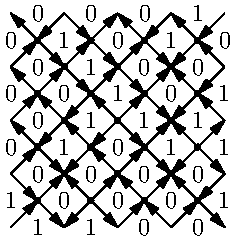
\includegraphics{Pictures/exemple8Kbar.pdf} 
\hspace{10mm}
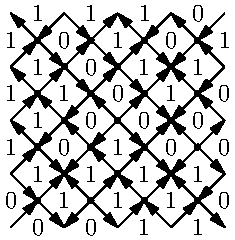
\includegraphics{Pictures/exemple8Kbar2.pdf} 
\end{center}
\caption{An orientation $O$ and its two possible 2-colorings.}\label{fig:col}
\end{figure}

Let us set $q = a/(a+c)$ and $r = b/({b+d})$, and consider the PCA $A_8$ defined in Section~\ref{sec:introExample}. We denote $\mathcal{F}_k$ the law of its space-time diagram $G(A_8,\pi_p)$ under its invariant measure $\pi_p$ restricted to $G_k$.

\begin{proposition}
[Lemma~5.4 and Proposition~1.3 of~\cite{Casse17}]
If $C \sim \mathcal{F}_k$, then $\mathcal{C}_8(C) \sim {\mathbb P}_W$.
\end{proposition}

This proposition is the first application of PCA with memory two in the literature. One can check that the PCA $A_8$ satisfies~\Cond~\ref{cond-pm} with $p(0)=p(1)=1/2$. Theorem~\ref{theo:ergo} implies that this PCA is ergodic. When $n \to \infty$, the center of the square has the same behaviour whatever the boundary conditions are~\cite[Proposition~1.6]{Casse17}.

Note that in what precedes, we have assumed that the weights satisfy the relation $a+c=b+d$. If we now assume that they rather satisfy $a+d=b+c$, we can design a PCA that, when iterated from left to right (or equivalently, from right to left), generates configurations distributed according to the required distribution ${\mathbb P}_W$. When $a=b$ and $c=d$, so that both relations are satisfied, we obtain $q=r$, and the dynamics is $D_4$-reversible.

\subsection{Enumeration of directed animals} \label{sec:animals}
In this section, we give a new proof about a known result (Lemma~\ref{lem:eq}) about enumerations of directed animals. Our new proof is based on the fact that, to any PCA with memory 2 with an HZMC invariant law, one can associate a PCA with memory 1 with the same invariant law.

A directed animal on the square lattice (resp. on the triangular lattice) is a set $A \subset \Z_{e}^2$ such that $(0,0) \in A$ and, for any $z \in A$ there exists a directed path $w=((0,0) = x_0, x_1, \dots, x_{m-1}, x_m=z)$ such that, for any $1 \leq k \leq m$,
\[
x_k-x_{k-1} \in \{u,v\} (\text{resp.}\{u,v,u+v\}),
\]
see Figure~\ref{figure:da} for an illustration on the triangular lattice. Let us denote by $\mathcal{A}_S$ (resp.~$\mathcal{A}_T$) the set of directed animals on the square (resp. triangular) lattice.

\begin{figure}\label{figure:da}
\begin{center}
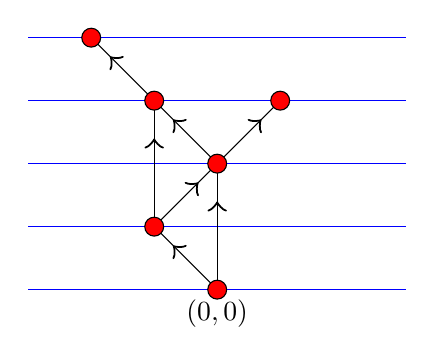
\begin{tikzpicture}[scale=0.8]
\foreach \y in {0,1,2,3,4} \draw[blue] (-3,\y) -- (3,\y) ;
\foreach \x in {0} \foreach \y in {2} {\draw[->-] (\x,\y-2) -- (\x,\y) ;}
\foreach \x in {-1} \foreach \y in {3} {\draw[->-] (\x,\y-2) -- (\x,\y) ;}
\foreach \x in {-1} \foreach \y in {3} {\draw[->-] (\x+1,\y-1) -- (\x,\y) ;}
\foreach \x in {-1} \foreach \y in {1} {\draw[->-] (\x+1,\y-1) -- (\x,\y) ;}
\foreach \x in {-2} \foreach \y in {4} {\draw[->-] (\x+1,\y-1) -- (\x,\y) ;}
\foreach \x in {0} \foreach \y in {2} {\draw[->-] (\x-1,\y-1) -- (\x,\y) ;}
\foreach \x in {1} \foreach \y in {3} {\draw[->-] (\x-1,\y-1) -- (\x,\y) ;}
\node[below] at (0,0) {$(0,0)$};
\draw [fill=red] (0,0) circle [radius=0.15];
\draw [fill=red] (-1,1) circle [radius=0.15];
\draw [fill=red] (0,2) circle [radius=0.15];
\draw [fill=red] (-1,3) circle [radius=0.15];
\draw [fill=red] (-2,4) circle [radius=0.15];
\draw [fill=red] (1,3) circle [radius=0.15];
\end{tikzpicture}
\hspace{2cm}
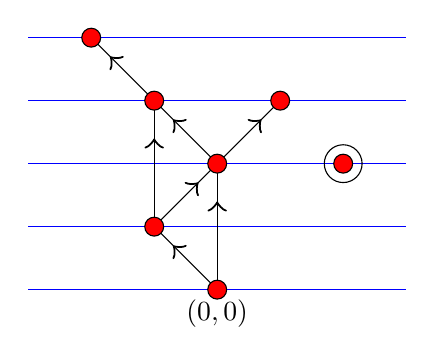
\begin{tikzpicture}[scale=0.8]
\foreach \y in {0,1,2,3,4} \draw[blue] (-3,\y) -- (3,\y) ;
\foreach \x in {0} \foreach \y in {2} {\draw[->-] (\x,\y-2) -- (\x,\y) ;}
\foreach \x in {-1} \foreach \y in {3} {\draw[->-] (\x,\y-2) -- (\x,\y) ;}
\foreach \x in {-1} \foreach \y in {3} {\draw[->-] (\x+1,\y-1) -- (\x,\y) ;}
\foreach \x in {-1} \foreach \y in {1} {\draw[->-] (\x+1,\y-1) -- (\x,\y) ;}
\foreach \x in {-2} \foreach \y in {4} {\draw[->-] (\x+1,\y-1) -- (\x,\y) ;}
\foreach \x in {0} \foreach \y in {2} {\draw[->-] (\x-1,\y-1) -- (\x,\y) ;}
\foreach \x in {1} \foreach \y in {3} {\draw[->-] (\x-1,\y-1) -- (\x,\y) ;}
\node[below] at (0,0) {$(0,0)$};
\draw [fill=red] (0,0) circle [radius=0.15];
\draw [fill=red] (-1,1) circle [radius=0.15];
\draw [fill=red] (0,2) circle [radius=0.15];
\draw [fill=red] (-1,3) circle [radius=0.15];
\draw [fill=red] (-2,4) circle [radius=0.15];
\draw [fill=red] (1,3) circle [radius=0.15];
\draw [fill=red] (2,2) circle [radius=0.15];
\draw (2,2) circle [radius=0.3];
\end{tikzpicture}
\caption{The set on the left is a directed animal on the triangular lattice, while the set on the right is not.}
\end{center}
\end{figure}


The \emph{area} of an animal $A$ is the cardinal of $A$ and the \emph{perimeter} of an animal $A$ is the cardinal of $P(A) = \{x : x \notin A, \{x\} \cup A \text{ is a directed animal}\}$. Let us introduce the generating functions of directed animals enumerated according to their area, on the square lattice and on the triangular lattice:
\begin{equation*}
G_S(z) = \sum_{A \in \mathcal{A}_S} z^{|A|} \qquad \qquad G_T(z) = \sum_{A \in \mathcal{A}_T} z^{|A|}.
\end{equation*}
The computation of these series was done by Dhar in 1982 via the study of hard-particles model~\cite{Dhar82}. Here, we will present this work using PCA, see also~\cite{mm_tcs} for details. Let us introduce the binary state PCA $B_S$ with memory one, and the binary state PCA $B_T$ with memory two, defined respectively by the following transition kernels:
\[
T_S(a,b;1) =
\begin{cases}
p_S & \text{if } a=b=0,\\
0 & \text{else}.
\end{cases}
\qquad T_T(a,b,c;1) =
\begin{cases}
p_T & \text{if} \; a=b=c=0,\\
0 & \text{otherwise}.
\end{cases}
\]
The following Theorem~\ref{theo:Dhar82} connects the generating functions $G_S$ and $G_T$ with these~PCA.

\begin{theo}[\cite{Dhar82,BousquetMelou98,LBM07}] \label{theo:Dhar82}
For any $p_S, p_T\in (0,1)$, let $(\eta_S(i,t): (i,t) \in \Z_{e}^2)$ and $(\eta_T(i,t): (i,t) \in \Z_{e}^2)$ be respectively the space-time diagram of $B_S$ and $B_T$ under their invariant probability measures. Then,
\begin{equation*}
\Pbb\left(\eta(0,0) = 1 \right) = - G_S(-p_S) \qquad \Pbb\left(\eta(0,0) = 1 \right) = - G_T(-p_T).
\end{equation*}
\end{theo}

In the case of directed animal on the square lattice, it is well known that $B_S$ has a simple $(F,B)$-HZMC invariant measure, that can be computed explicitly, see~\cite{BousquetMelou98,CM15,Dhar82,LBM07}. Note also that the ergodicity of $B_S$, for any choice of $p_S\in(0,1)$, was proven in~\cite{hmm}. Using Proposition~\ref{prop:Casse17}, one obtain that if $ p_S = \frac{p_T}{1+p_T}$, then \Cond~\ref{cond:DU-HZMC} holds, so that the same $(F,B)$-HZMC is also an invariant measure of $B_T$. We thus obtain the following Lemma~\ref{lem:eq} (although $B_S$ and $B_T$ do not have positive rates, we can easily extend our sufficient conditions to them).

\begin{lemm}\label{lem:eq}
We have the following:
\begin{equation}\label{eq:eq}
G_T\left(\frac{z}{1+z}\right) = G_S(z).
\end{equation}
\end{lemm}

This allows to obtain the expression of the area generating function of directed animals on the triangular lattice from the one on the square lattice. We give below the two expressions of $G_S$ and $G_T$.

\begin{theo}[\cite{BousquetMelou98,Dhar82}]
The area generating function of directed animals on the square lattice and on the triangular lattice are respectively given by:
\begin{equation*}
G_S(z) = \frac{1}{2} \left(\left(1 - \frac{4z}{1+z} \right)^{-1/2} - 1 \right) \quad \text{ and } \quad G_T(z) = \frac{1}{2} \left(\left(1 - 4z \right)^{-1/2} - 1 \right).
\end{equation*}
\end{theo}

The same questions can be asked for the enumeration according to area and perimeter, but in this case we have no explicit description of the invariant measures of the PCA involved. For more references on the question, see~\cite{LBM07,mm_tcs}.

\subsection{Parallel TASEP of order two} \label{sec:TASEP}

The TASEP (Totally ASymmetric Exclusion Process) describes the evolution of some particles that go from the left to the right on a line without overtaking. There are various kinds of TASEP models, with discrete or continuous time and space, and one or more types of particles. We refer the interested readers to the following articles~\cite{BC15,belitsky,gray} for the description of some models with discrete time and space. Here, we present a new (to the best knowledge of the authors) generalization of TASEP called TASEP of order two on real line and discrete time.

The TASEP presented here models the behaviour of an infinite number of particles (indexed by $\ZZ$) on the real line, that move to the right, and that do not bypass and do not overlap. For $i,t\in\Z$, we denote by $x_i(t)\in \RR$ the position of particle $i$ at time $t$. Time is discrete, and at time $t$, each particle $i\in\ZZ$ moves with a random speed $v_i(t)$, independently of the others. The random speed $v_i(t)$ depends on the distance $x_{i+1}(t)-x_i(t)$ between the particle $i$ and the particle $i+1$ in front of it, and of the speed $v_{i+1}(t-1)=x_{i+1}(t)-x_{i+1}(t-1)$ of the particle $i+1$ at time $t-1$. Formally, the evolution of $(x_i(t))_{i \in \ZZ}$ is defined by:
\begin{equation*}
\forall i\in\ZZ, \quad x_i(t+1) = x_i(t) + v_i(t),
\end{equation*}
where $v_i(t)$ is random and distributed following $\mu_{(x_{i+1}(t)-x_i(t),v_{i+1}(t-1))}$, a probability distribution on $\RR^+$, and $(v_i(t))_{i \in \ZZ}$ are independent, knowing $(x_i(t))_{i\in \ZZ}$ and \linebreak$(x_{i}(t-1))_{i \in \ZZ}$.



It is known that TASEP with discrete time can be represented by PCA~\cite{Casse16,mm_tcs}. We adopt the approach presented in~\cite{Casse16} to show that the TASEP of order two can be represented by a PCA with memory two: take $\eta(i,t) = x_i(t)$, then $(\eta(i,t) : i \in \ZZ, t \in \NN)$ is the space-time diagram of a PCA with memory two whose transition kernel $T$ is, for any $a \in \RR, x,y,v \in \RR^+$,
\begin{equation*}
T(a,a+x,a+x+y;a+v) = \mu_{(x+y,y)}(v).
\end{equation*}


Now, we will focus as an example on the simplest case where $v \in \{0,1\}$ a.s. and particles move on the integer line (for any $i\in\ZZ,t\in\NN$, $x_i(t) \in \ZZ$). The constraints we have on $T$ are the following:
\begin{itemize}
\item $T(a,a+1,a+1;a) =1$ for any $a\in \ZZ$ (and $T(a,b,b+i;c)$ can take any value if $i \neq 0,1$ or $b \leq a$),
\item $T(a,a+k,a+k+i;c) = 0$ for any $a$, $k \geq 0$, $i \in \{0,1\}$ and $c \notin \{a,a+1\}$,
\item $T(a,a+k,a+k+i;a) = T(b,b+k,b+k+i;b)$ for any $k\geq 1$, $i \in \{0,1\}$, $a,b \in \ZZ$.
\end{itemize}
The first two points mean that the next position has to be empty for a particle to move, and that a particle can only move of one unit forward. The last point is an hypothesis of translation invariance. Hence, the PCA can be described by the transitions $(T(0,k,k;0))_{k \geq 2}$ and $(T(0,k,k+1;0))_{k \geq 1}$. Although this PCA is not with positive rates and does not admit an invariant measure, it has some interesting properties that permit to find invariant measures for the parallel TASEP.

The model above is reminiscent of $q$-TASEP models as defined in~\cite{BC15}. In particular, the discrete time \emph{Bernoulli $q$-TASEP} can be interpreted as a TASEP of order two with a time change. In contrast to our model, the number of particles is assumed to be finite, and at each time step, the positions of the particles are updated successively from right to left: each particle can move by one unit, with a probability that depends both on the length of the gap with the foregoing particle and on the fact that the jump of the foregoing particle did occur or not. The \emph{Poisson $q$-TASEP} is a continuous time TASEP, but it also shares the property that the rate at which particles jump forward is modulated by the distance to the next particle, which is also the case of the discrete time \emph{geometric $q$-TASEP}. In this last model, particles can move by several units in one time step. It follows that the geometric $q$-TASEP is tightly related to TAZRP models, and as we may detail in a future work, the PCA approach can be extended to these models.

\begin{figure}
\begin{center}
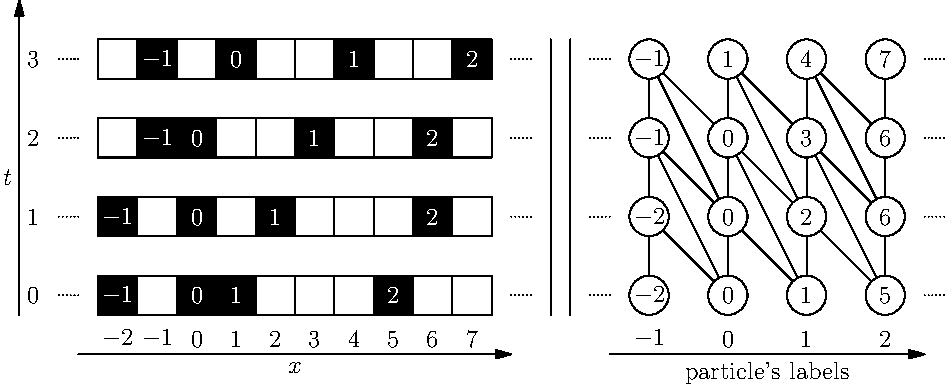
\includegraphics[scale=0.8]{Pictures/TASEP.pdf} 
\end{center}
\caption{On the left, the classical representation of a TASEP: a white square is an empty square; a black square is a square that contains a particle, the white number is the label of this particle. On the right, the PCA that represents this TASEP; each column represents the trajectory of a particle.}
\end{figure}

The first result of this section is about the fact that there exists a family of $(F,B)$-HZMC that is stable by this PCA. First, let us define a $(q,p)$-HZMC for any probability $q$ and $p$ on $\ZZ$: a $(q,p)$-HZMC is a $(F,B)$-HZMC such that, for any $a,k \in \ZZ$, $F(a;a+k) = q(k)$ and $B(a;a+k) = p(k)$.

\begin{lemm}\label{lem:TASEP}
For any transition kernel $T$, if there exist $p$ a probability on $\NN^*$ and $q$ on $\{0,1\}$ such that, for any $k \geq 1$,
\begin{equation}\label{eq:TASEP}
p(k) q(1) T(0,k,k+1;0) + p(k+1) q(0) T(0,k+1,k+1;0) = p(k+1)q(0)
\end{equation}
then if we start under the law such that $(\eta_0,\eta_1)$ is a $(q,p)$-HZMC with $\eta_0(0)=0$ a.s., then any double line $(\eta_t,\eta_{t+1})$ is also distributed as a $(q,p)$-HZMC but the starting point is now $\eta_t(0)$ with
\[
\Pbb\left(\eta_t(0) = k\right) = \binom{t}{k} q(1)^k q(0)^{t-k}.
\]
\end{lemm}

Note that~\eqref{eq:TASEP} also implies
\begin{equation}\label{eq2:TASEP}
p(k) q(1) T(0,k,k+1;1) + p(k+1) q(0) T(0,k+1,k+1;1) = p(k)q(1),
\end{equation}
both equations being equivalent to:
\begin{equation}\label{eqequiv:TASEP}
p(k) q(1) T(0,k,k+1;0) = p(k+1) q(0) T(0,k+1,k+1;1).
\end{equation}
These two conditions~\eqref{eq:TASEP} and~\eqref{eq2:TASEP} are similar to \Cond~\ref{cond:DU-HZMC} of Proposition~\ref{prop:Casse17}.

\begin{proof}
The proof is done by induction on $t\in\NN$. For $t=0$, we assume that $(\eta_0,\eta_1)$ is a $(q,p)$-HZMC with $\eta_0(0)=0$ a.s.
Now, let us suppose that $(\eta_t,\eta_{t+1})$ is a $(q,p)$-HZMC with $ \Pbb\left(\eta_t(0) = k\right) = \binom{t}{k} q(1)^k q(0)^{t-k}$. Then, by conditioning on the possible values $(a_i)_{0 \leq i \leq k+1}$ for $(\eta_t(i))_{0 \leq i \leq k+1}$, we obtain that the finite dimensional laws of $(\eta_{t+1},\eta_{t+2})$ are given by:
\begin{align*}
& \Pbb\left((\eta_{t+1}(i)=b_i)_{0 \leq i \leq k},(\eta_{t+2}(i)=c_i)_{0 \leq i \leq k-1}\right)\\
&= \sum_{a_0,\dots,a_{k+1}}\!\!\binom{t}{a_0} q(1)^{a_0} q(0)^{t-a_0} q(b_0\!-\!a_0)\!\prod_{i=0}^{k-1} p(a_{i+1}\!-\!b_i) q(b_{i+1}\!-\!a_{i+1}) T(b_i,a_{i+1},b_{i+1};c_i) \\
&= \left(\sum_{a_0 } \binom{t}{a_0} q(1)^{a_0} q(0)^{t-a_0} q(b_0-a_0)\right) \\
&\mkern 210mu \left(\prod_{i=0}^{k-1} \; \sum_{a_{i+1} } p(a_{i+1}-b_i) q(b_{i+1}-a_{i+1}) T(b_i,a_{i+1},b_{i+1};c_i)\!\!\right).
\end{align*}
Since the only non-zero terms correspond to $a_i\in\{b_i,b_i-1\}$, the left parenthesis is equal to:
\[
\sum_{a_0\in\{b_0,b_0-1\}} \binom{t}{a_0} q(1)^{a_0} q(0)^{t-a_0} q(b_0-a_0)=\binom{t+1}{b_0} q(1)^{b_0} q(0)^{t+1-b_0},
\]
and the right one to:
\begin{align*}
&\prod_{i=0}^{k-1} \; \sum_{a_{i+1}\in\{b_{i+1},b_{i+1}-1\}} p(a_{i+1}-b_i) q(b_{i+1}-a_{i+1}) T(b_i,a_{i+1},b_{i+1};c_i)\\
&\quad=\prod_{i=0}^{k-1} \; \sum_{a_{i+1\in\{b_{i+1},b_{i+1}-1\}}} p(a_{i+1}-b_i) q(b_{i+1}-a_{i+1}) T(0,a_{i+1}-b_i,b_{i+1}-b_i;c_i-b_i) \\
&\quad=\prod_{i=0}^{k-1} p(b_{i+1}-c_i) q(c_i-b_i), \quad \text{using~\eqref{eq:TASEP} and~\eqref{eq2:TASEP}}.\qedhere
\end{align*}
\end{proof}

We can remark that $q$ is the speed law of a particle under the stationary regime and $p$ the distance law between two successive particles (to be precise the left one at current time $t$ and the right one at previous time $t-1$).



\begin{theo}\label{theo:TASEP}
For any $T$, for any distribution $q$ on $\{0,1\}$ such that
\begin{equation}\label{eq:TASEPZ}
Z = \sum_{k=0}^\infty \left(\frac{q(1)}{q(0)}\right)^k \prod_{m=1}^k \frac{T(0,m,m+1;0)}{T(0,m+1,m+1;1)} < \infty,
\end{equation}
there exists a unique distribution $p$ on $\NN^*$ such that~\eqref{eq:TASEP} hold.

Moreover, this distribution $p$ is, for any $k \geq 1$,
\begin{equation}\label{eq:TASEPp}
p(k) = \frac{\displaystyle \left(\frac{q(1)}{q(0)}\right)^{k-1} \prod_{m=1}^{k-1} \frac{T(0,m,m+1;0)}{T(0,m+1,m+1;1)}}{Z}.
\end{equation}
\end{theo}

\begin{proof}
Let $q$ be a probability measure on $\{0,1\}$. By~\eqref{eqequiv:TASEP}, we have
\begin{equation}\label{eq:TASEPind}
\forall k\geq 1, \quad p(k+1) = p(k) \frac{T(0,k,k+1;0)}{T(0,k+1,k+1;1)} \frac{q(1)}{q(0)}.
\end{equation}
By induction, we obtain
\begin{equation*}
\forall k\geq 1, \quad p(k+1)=\left(\frac{q(1)}{q(0)}\right)^k \prod_{m=1}^k \frac{T(0,m,m+1;0)}{T(0,m+1,m+1;1)} p(1)
\end{equation*}
As $\sum_{k\in\NN^*} p(k) = 1$, we need~\eqref{eq:TASEPZ}. In that case, \eqref{eq:TASEPp} follows.
\end{proof}

In the classical case of parallel TASEP (presented in~\cite[Sections~2.3 \& 4.3]{mm_tcs},~\cite[Section~3.3]{Casse16}), we have
\begin{equation}\label{eq:classTASEP}
T(0,k,k+1;1) = T(0,k+1,k+1;1) = p.
\end{equation}
With Theorem~\ref{theo:TASEP}, we recover the invariant measures of the classical parallel TASEP and can express the one of the generalized TASEP as a renewal process.


\begin{coro}
For any distribution $q$ on $\{0,1\}$ such that~\eqref{eq:TASEPZ} holds and $p$ (given by~\eqref{eq:TASEPp}, with $p(0)=0$) has a finite mean, the TASEP of order 2 has an invariant measure on $\{0,1\}^\ZZ \times \{0,1\}^\ZZ$ such that on the same line, the distance between two consecutive $1$s are i.i.d. and distributed according to $\gamma$ with, for any $k \geq 1$, $\gamma(k) = q(0) p(k) + q(1)p(k-1)$.
\end{coro}

This example goes beyond our previous framework for many reasons. First, the PCA does not have positive rates. Second, studying the invariant measures of this PCA is not interesting because they only correspond to states where nobody moves. That is why we have focused here on families of distributions that are stable by the PCA rather than on only one invariant distribution. And by studying carefully the eigenvectors on the good subspaces, we are able to solve the algebraic issues. This provides some interesting results on a PCA with an infinite alphabet, involving a family of $(F,B)$-HZMC laws (with $F \neq B$), whereas our main explicit results on PCA involve general $(F,B)$-HZMC measures but on an alphabet of size $2$, or PCA with a general alphabet but with an invariant $(F,F)$-HZMC (see the end of Section~\ref{sec:invHZMC} and Section~\ref{sec:general}).

\section{The binary case}\label{sec:binary}

In this section, we specify the conditions obtained in Section~\ref{sec:rqrPCA} to the case of a binary symbol set $S=\{0,1\}$.

\begin{prop}\label{prop:condbinaire}
For a binary symbol set $S=\{0,1\}$,
\begin{enumerate}
\item \label{list7.1.1}\Cond~\ref{cond-pm} is equivalent to\\
\begin{cond}\label{cond1:2col}
$
\forall a,c\in S,\, p(0)T(a,0,c;1)=p(1)T(a,1,c;0).
$
\end{cond}
\item \label{list7.1.2}\Cond~\ref{cond:r1rev} is equivalent to\\
\begin{cond}\label{cond2:2col}
$
\forall a,b\in S,\, p(0)T(a,b,0;1)=p(1)T(a,b,1;0).
$
\end{cond}
\item \label{list7.1.3}\Cond~\ref{cond:r3rev} is equivalent to\\
\begin{cond}\label{cond3:2col}
$
\forall b,c\in S,\,p(0)T(0,b,c;1)=p(1)T(1,b,c;0).
$
\end{cond}
\end{enumerate}
\end{prop}

\begin{proof}
In the binary case, \Cond~\ref{cond-pm} reduces to: 
\[
\forall a,c\in S, \; p(1)=p(0)T(a,0,c;1)+p(1)T(a,1,c;1),
\]
which is itself equivalent to \Cond~\ref{cond1:2col}. The proof is analogous for \Cond~\ref{cond2:2col} and \Cond~\ref{cond3:2col}.
\end{proof}

Let $p$ be a probability measure on $S=\{0,1\}$. If we specify some results of Table~\ref{table:pres} to the case $|S|=2,$ we obtain
\begin{align*}
& \dim \left(\triang{S}{p} \right) = \dim \left(\{A \in \triang{S}{p} : A \text{ is $h$-reversible}\} \right) = 4,\\
& \dim \left(\{A \in \triang{S}{p} : A \text{ is $v$-reversible}\} \right) = \dim \left(\{A \in \triang{S}{p} : A \text{ is $r^2$-reversible}\} \right) = 3,\\
& \dim \left(\{A \in \triang{S}{p} : A \text{ is $D_4$-quasi-reversible}\} \right) \\
&\mkern 280mu =\dim \left(\{A \in \triang{S}{p} : A \text{ is $D_4$-reversible}\} \right) = 1.
\end{align*}

In this section, we describe more precisely these different sets, which give an alternative proof of the value of their dimension, in the binary case. First, the next result shows that in the binary case, the sets above having the same dimension are equal.

\begin{prop}
Let $p$ be any positive probability on $S=\{0,1\}$, and let $A\in\triang{S}{p}$. Then, we have the following properties.
\begin{enumerate}
\item \label{list7.2.1}$A$ is $h$-reversible.
\item \label{list7.2.2}$A$ is $v$-reversible iff $A$ is $r^2$-reversible.
\item \label{list7.2.3}$A$ is $D_4$-quasi-reversible iff $A$ is $D_4$-reversible.
\end{enumerate}
\end{prop}

\begin{proofc}
\begin{proof}[{\eqref{list7.2.1}}] Since $A$ is in $\triang{S}{p}$, $A$ is $h$-quasi-reversible, and the transition kernel $T_h$ of its $h$-reverse satisfies, for any $a,b,c,d \in S$,
\[
T_h(a,d,c;b) = \frac{p(b)}{p(d)} T(a,b,c;d).
\]
For $b=d,$ this gives $T_h(a,b,c;d)=T(a,b,c;d),$ and for $b\not=d$, \Cond~\ref{cond1:2col} provides the result.
\let\qed\relax
\end{proof}
\begin{proof}[{\eqref{list7.2.2}}]It is a corollary of 1. Indeed, if $A$ is in $\triang{S}{p}$ and $v$-reversible, then it is $h$ and $v$-reversible, and so also $r^2 = v \circ h$-reversible. And conversely, if it is $r^2$-reversible, then it is $v=r^2\circ h$-reversible.
\let\qed\relax
\end{proof}
\begin{proof}[{\eqref{list7.2.3}}]This will be a consequence of Proposition~\ref{theo:drev2col}. \qedhere
\end{proof}
\let\qed\relax
\end{proofc}

As a consequence of Proposition~\ref{prop:condbinaire}, we obtain the following descriptions of binary PCA having an invariant HZPM.

\begin{prop}\label{theo:r-rev2col}
Let $A$ be a PCA with transition kernel $T$ (with positive rates). Then $A$ has an invariant HZPM iff

\begin{cond} \label{cond:HZPM2}
there exists $k \in\mathopen]0,\infty[$ such that for any $a,c \in S$,
\[
\frac{T(a,1,c;0)}{T(a,0,c;1)} = k.
\]
\end{cond} More explicitly, this is equivalent to the following condition.


\begin{cond} \label{cond:HZPM2-exp}
there exists $k \in\mathopen]0,\infty[$ and
\[
\begin{cases}
q_{0,0},q_{0,1},q_{1,0},q_{1,1} \in(0,1)&\text{if } k \in (0,1]\\
q_{0,0},q_{0,1},q_{1,0},q_{1,1} \in(1-k^{-1},1)&\text{if } k \in [1,\infty\!)
\end{cases}
\]
such that, for any $a,c\in S$,
\begin{align*}
&T(a,0,c;0) = q_{a,c},\\
&T(a,1,c;0) = k (1-q_{a,c}) = k-kq_{a,c}.
\end{align*}
\end{cond}

In that case, the $p$-HZPM invariant is $(p(0),p(1))$ where
\[ 
p(1) = 1 - p(0)\!=\!\frac{1}{1+k}.
\]
\end{prop}

\begin{proof}
The PCA $A$ has an invariant HZPM iff there exists a probability $p$ on $S$ such that \Cond~\ref{cond1:2col} is satisfied, which can easily be shown to be equivalent to the above conditions.
\end{proof}
\goodbreak

\begin{prop}\label{prop:r2rev2}
Let $p$ be a positive probability on $S$, and let $k=p(0)/p(1)$.
%
Then, $A$ is a $r$-quasi-reversible PCA of $\triang{S}{p}$ iff

\textnormal{\begin{cond} \label{cond:unorder3}
There exist
\[
\begin{cases}
q_0,q_1 \in (0,1) & \text{if } k \in (0,1]\\
q_0,q_1 \in (1-k^{-1},1-k^{-1}+k^{-2}) & \text{if } k \in [1,\infty)
\end{cases}
\]
such that, for any $a\in S$:
\begin{align*}
&T(a,0,0;0) = q_a,\\
&T(a,0,1;0) = T(a,1,0;0) = k (1-q_c) = k-kq_a\\
&T(a,1,1;0) = k (1-k(1-q_c)) = k-k^2+k^2q_a.
\end{align*}
\end{cond}}

Similarly, $A$ is a $r^{-1}$-quasi-reversible PCA of $\triang{S}{p}$ iff

\textnormal{\begin{cond} \label{cond:unorder4}
There exist
\[
\begin{cases}
q_0,q_1 \in (0,1) & \text{if } k \in (0,1]\\
q_0,q_1 \in (1-k^{-1},1-k^{-1}+k^{-2}) & \text{if } k \in [1,\infty)
\end{cases}
\]
such that, for any $c \in S$:
\begin{align*}
&T(0,0,c;0) = q_c,\\
&T(0,1,c;0) = T(1,0,c;0) = k (1-q_c) = k-kq_c\\
&T(1,1,c;0) = k (1-k(1-q_c)) = k-k^2+k^2q_c.
\end{align*}
\end{cond}}
\end{prop}

\begin{proof}
We prove the first statement. Let $A$ be a $r$-quasi-reversible PCA in $\triang{S}{p}$.
Then $T$ satisfies \Cond~\ref{cond1:2col} and~\ref{cond2:2col}, meaning that for any $a,b,c \in S$,
\[
\frac{T(a,1,c;0)}{T(a,0,c;1)} = \frac{T(a,b,1;0)}{T(a,b,0;1)} = k = \frac{p(0)}{p(1)}.
\]
Taking $b=c=0$, we find, for any $a \in S$,
\[
T(a,1,0;0) = T(a,0,1;0) = k T(a,0,0;1)
\]
and taking $b=c=1$, we find that for any $a \in S$,
\[
T(a,0,1;1) = T(a,1,0;1) = k^{-1} T(a,1,1;0).
\]
Hence, for any $a \in S$, we obtain
\[
T(a,1,1;0) = k (1-T(a,0,1;0)) = k (1 - k (1-T(a,0,0;0))).
\]

Then, every $T(a,b,c;d)$ can be express in terms of $T(0,0,0;0) =q_0$, $T(0,0,1;0) =q_1$ and $k$, which gives \Cond~\ref{cond:unorder3}, and the range of $q_0,q_1$ is deduced from the fact that, for any $a,b,c,d \in S$, $T(a,b,c;d) \in (0,1)$.

Conversely, let $A$ be such that \Cond~\ref{cond:unorder3} holds. Then \Cond~\ref{cond1:2col} and~\ref{cond2:2col} hold, so $A \in \triang{S}{p}$ and $A$ is $r$-quasi-reversible.
\end{proof}
%%\pagebreak

\begin{prop}\label{theo:drev2col}
Let $p$ be a positive probability on $S$, and let $k=p(0)/p(1)$.

Then, $A$ is a $\{r,r^{-1}\}$-quasi-reversible PCA of $\triang{S}{p}$ iff

\textnormal{\begin{cond} \label{cond:unorder2}
There exists
\[
\begin{cases}
q_0 \in (0,1) & \text{if } k \in (0,1]\\
q_0 \in (1-k^{-1}+k^{-2}-k^{-3},1-k^{-1}+k^{-2}) & \text{if } k \in [1,\infty)
\end{cases}
\]
such that
\begin{align*}
&T(0,0,0;0) = q_0,\\
&T(0,0,1;0) = T(0,1,0;0) = T(1,0,0;0) = k (1-q_0) = k-kq_0\\
&T(0,1,1;0) = T(1,1,0;0) = T(1,0,1;0) = k (1-k(1-q_0)) = k-k^2+k^2q_0\\
&T(1,1,1;0) = k(1-k(1-k(1-q_0))) = k -k^2 + k^3 -k^3q_0.
\end{align*}
\end{cond}}

Moreover, in that case, $A$ is $D_4$-reversible.
\end{prop}

\begin{proof}
The PCA $A$ is a $\{r,r^{-1}\}$-quasi-reversible PCA of $\triang{S}{p}$ iff \Cond~\ref{cond1:2col}, \ref{cond2:2col} and~\ref{cond3:2col} are satisfied, which can easily be shown to be equivalent to the above condition.
Now, we prove the $D_4$-reversibility of $A$. First, $A$ is symmetric, so $A$ is $v$-reversible. Second, it is easy to check that $T_r=T$, so that $A$ is $r$ and $v$-reversible. By~\eqref{list2.7.5} of Proposition~\ref{prop:obvious}, $A$ is $D_4$-reversible.
\end{proof}

\begin{exam}
Let us consider the special case when $p$ is the uniform distribution on $S$, meaning that $p(0)=p(1)=1/2$. Then, $k=1$, and the family of PCA above corresponds to:
\[
\forall a,b,c,d\in S, \quad T(a,b,c;d)=
\begin{cases}
\;\; q_0  &\text{ if } \; d=a+b+c \mod 2\\
1-q_0  &\text{ otherwise. }
\end{cases}
\]
In the deterministic case ($q_0=1$), we get a linear CA. Such CA have been intensively studied. Here, in the probabilistic setting, the PCA we obtain can be seen as noisy versions of that linear CA (with a probability $1-q_0$ of doing an error, independently for different cells). This is a special case of the $8$-vertex PCA, with $p=r$.
\end{exam}

\begin{exam}\label{exemple:binaire}
Let us consider the probability distribution on $S$ given by $p(0) = 1/3$ and $p(1) = 2/3$, so that $k=2$. When specifying \Cond~\ref{cond:unorder3} to $q_0=3/4$ and $q_1 = 4/5$, we obtain
\begin{align*}
T(0,0,0;0) &= 3/4, & T(1,0,0;0) &= 4/5,\\
T(0,0,1;0) &= T(0,1,0;0) = 1/8, & T(1,0,1;0) &= T(1,1,0;0) = 1/10,\\
T(0,1,1;0) &= 7/16, & T(1,1,1;0) &= 9/20.
\end{align*}
The PCA $A$ of transition kernel $T$ is $r$-quasi-reversible, but one can check that it does not satisfy \Cond~\ref{cond3:2col}, so that it is not $r^{-1}$-quasi-reversible. So, $T_r$ does not belong to $\triang{S}{p}$, and following the argument developed in Section~\ref{sec:notmarkov}, $T_r$ does not have an invariant HZMC either. Nevertheless, one can exactly compute the marginals of its invariant measure $\mu$, see~\eqref{calcul_expl1} and~\eqref{calcul_expl2}. The transitions of $T_r$ are the following ones:
\begin{align*}
T_r(0,0,0;0) &= 3/4,& T_r(1,0,0;0) &= 1/8,\\
T_r(0,0,1;0) &= 1/8,& T_r(1,0,1;0) &= 7/16,\\
T_r(0,1,0;0) &= 4/5,& T_r(1,1,0;0) &= 1/10,\\
T_r(0,1,1;0) &= 1/10,& T_r(1,1,1;0) &= 9/20.
\end{align*}
\end{exam}


\section{Extension to general alphabet} \label{sec:general}

We now present some extensions of our methods and results to general sets of symbols. First of all, we extend the definition of PCA to any Polish space $S$, as it has been done in~\cite{Casse16} for PCA with memory one. The transition kernel $T$ of a PCA with memory two must now satisfy
\begin{itemize}
\item for any Borel set $D \in \borel{S}$, the map
\[
\app{T_D}{S^3}{\RR}{(a,b,c)}{T(a,b,c;D)}
\]
is $\mathcal{B}(S^3)$-measurable;
\item for any $a,b,c\in S$, the map
\[
\app{T_{a,b,c}}{\borel{S}}{\RR}{D}{T(a,b,c;D)}
\]
is a probability measure on~$S$.
\end{itemize}

For any $\sigma$-finite measure $\mu$ on $S$, the transition kernel $T$ is said to be $\mu$-positive if, for $\mu^3$-almost every $(a,b,c)\in S^3$, $T(a,b,c;.)$ is absolutely continuous with respect to $\mu$ and $\mu$ is absolutely continuous with respect to $T(a,b,c;.)$. In that case, thanks to Radon--Nikodym theorem, we can define the density of $T$ with respect to $\mu$, that is a $\mu^4$-measurable positive function where, for $\mu^3$-almost every $(a,b,c)\in S^3$,
\begin{equation*}
t(a,b,c;d) = \frac{\text{d} T(a,b,c;\cdot\,)}{\text{d} \mu}(d)
\end{equation*}
where $ \frac{\text{d} T(a,b,c;\,\cdot\,)}{\text{d} \mu}$ is the Radon--Nikodym derivative of $T(a,b,c;\cdot\,)$ with respect to~$\mu$.

\begin{theo}
Let $\mu$ be any $\sigma$-finite measure on a Polish space $S$. Let $A$ be a PCA with a $\mu$-positive transition kernel $T$ on $S$. Then, $A$ has an invariant $\mu$-positive HZPM iff
\begin{cond} \label{cond:HZPM-polonais}
there exists a $\mu$-measurable positive function $p$ on $S$ such that, for $\mu^3$-almost every $(a,c,d) \in S^3$,
\begin{align*}
& p(d) = \int_E p(b) t(a,b,c;d) \diff{\mu(b)}\\ \text{and}\quad
& \mu(p) = \int_E p(b) \diff{\mu(b)} < \infty,
\end{align*}
where $t$ is the $\mu$-density of $T$.
\end{cond}

Then, the $P$-HZPM is invariant by $A$ where $p(\cdot)/\mu(p)$ is the $\mu$-density of $P$.
\end{theo}
\goodbreak

\begin{proof}
The proof follows the same idea as that of Theorem~\ref{theo:gen0}, except that we are now on a Polish space $S$. Let $A$ be a $\mu$-positive triangular PCA with alphabet $S$.

%\begin{itemize}
%\item[$\bullet$]
Suppose that $A$ has an invariant $\mu$-positive $P$-HZPM and that $(\eta_t,\eta_{t+1})$ follows a $P$-HZPM distribution. Then, for any $\tilde A,\tilde B, \tilde C,\tilde D \in \borel{S}$,
\begin{multline*}
\Pbb\left(\eta_t(i-1) \in \tilde A, \eta_{t+1}(i) \in \tilde D, \eta_t(i+1) \in \tilde C\right) \\
\begin{aligned}
& = \int_{\tilde A \times \tilde C \times \tilde D} p(a) p(c) p(d) \diff{\mu^3(a,c,d)} & \text{ on the one hand,}\\
& = \int_{\tilde A \times \tilde C \times \tilde D} \left(\int_S p(a) p(b) p(c) t(a,b,c;d) \diff{\mu(b)} \right) \diff{\mu^3(a,c,d)} & \text{ on the other hand.}
\end{aligned}
\end{multline*}
Hence, for $\mu$-almost $a,c,d \in S$,
\[
p(a) p(c) \int_S p(b) t(a,b,c;d) \diff{\mu(b)} = p(a) p(d) p(c)
\]
and so, as $p(a),p(c) > 0$ for $\mu$-almost $a,c\in S$, \Cond~\ref{cond:HZPM-polonais} holds.


%\item[$\bullet$]
Conversely, assume that \Cond~\ref{cond:HZPM-polonais} is satisfied, and that $(\eta_{t-1},\eta_t)$ follows a $\mu$-positive $P$-HZPM distribution. For some given choice of $n\in\Z_{t}$, let us denote: $X_i=\eta_{t-1}(n+1+2i), Y_i=\eta_{t}(n+2i), Z_i=\eta_{t+1}(n+1+2i),$ for $i\in \Z$, see Figure~\ref{fig:hzpm_proof} for an illustration. Then, for any $k\geq 1$, for any $\mu$-measurable Borel sets $B_0,B_1,\dots,B_k, C_0,\dots,C_{k-1}$,
\begin{align*}
& \Pbb\left((Y_i)_{0 \leq i \leq k} \in B_0\times \cdots \times B_k, (Z_i)_{0 \leq i \leq k-1} \in C_0 \times \cdots \times C_{k-1}\right) \\
& = \int_{C_0 \times \dots \times C_{k-1}} \int_{B_0 \times \dots \times B_{k}} \left(\prod_{i=0}^{k-1} \int_{S} t(y_i,x_{i},y_{i+1};z_i) p(x_{i}) \diff{\mu(x_{i})} \right) \nonumber \\
&\mkern 275mu p(y_0) \dots p(y_{k}) \diff{\mu(y_0,\dots,y_{k})} \diff{\mu(z_0,\dots,z_{k-1})}\\
& = \int_{C_0 \times \dots \times C_{k-1}} \int_{B_0 \times \dots \times B_{k}} \left(\prod_{i=0}^{k-1} p(z_{i}) \right) p(y_0) \dots p(y_{k}) \diff{\mu(y_0,\dots,y_{k})} \diff{\mu(z_0,\dots,z_{k-1})}
\end{align*}
thus, the $P$-HZPM distribution is invariant by $A$.
%\end{itemize}
\end{proof}

Now, the problem is reduced to finding eigenfunction associated to the eigenvalue~$1$ of some integral operator. If this problem is solved by Gauss elimination in the case of a finite space, this is more complicated in the general case. Indeed, such a function does not always exist, but, when it is the case, the solution is unique (up to a multiplicative constant), see the following lemma.

\begin{lemm}[{\cite[Theorem~6.8.7]{Durrett10}}]
Let $\mathcal{A}$ be an integral operator of kernel $m$:
\[
\mathcal{A}: f \to \left(\mathcal{A}(f) : y \to \int_S f(x) m(x;y) \diff \mu(x)\right).
\]
If $m$ is the $\mu$-density of a $\mu$-positive t. k. $M$ from $S$ to $S$, then $\mathcal{A}$ possesses at most one positive eigenfunction in $L^1(\mu)$ (up to a multiplicative constant).
\end{lemm}

Moreover, the previous results concerning the characterization of reversible and quasi-reversible PCA extend to PCA with general alphabet. The difference is that we are considering $\mu$-positive PCA and that \Cond~\ref{cond:r1rev} and~\ref{cond:r3rev} are respectively replaced by the two following Conditions~\eqref{cond18} and~\eqref{cond19}.

\begin{cond}\label{cond18}
for $\mu^3$-almost every $(a,b,d) \in S^3$, $\int_{S} p(c) t(a,b,c;d) \diff{\mu(c)} = p(d)$
\end{cond}

\begin{cond}\label{cond19}
for $\mu^3$-almost every $(b,c,d) \in S^3$, $\int_{S} p(a) t(a,b,c;d) \diff{\mu(a)} = p(d)$.
\end{cond}

Following the same idea as in~\cite{Casse16}, many results on PCA with invariant $(F,B)$-HZMC can also be generalized to PCA on general alphabets.

\section{Dimensions of the manifolds}\label{sec:dim}

In this section, we give the dimensions of $\triang{S}{p}$ and of its subsets of (quasi-) reversible PCA, as functions of the cardinal $n$ of the alphabet $S$ (see Table~\ref{table:pres}). But first, we need some results about dimensions of sets of matrices.

\subsection{Preliminaries: dimensions of sets of matrices with a given eigenvector}

Let $S$ be a finite set of size $n$, and let $u,v$ be two positive probabilities on $S$. We denote by $\mathcal{M}_S(u,v)$ the set of positive matrices $M = (m_{ij})_{i,j \in S}$ such that $M$ is a stochastic matrix and $uM=v$, i.e.
\begin{align*}
\mathcal{M}_S(u,v) = \quad \{ M = (m_{ij})_{i,j \in S} : & \quad \text{for any } i,j \in S,\ 0 < m_{ij} < 1;\\
& \quad \text{for any } i \in S,\ \sum_{j\in S} m_{ij} = 1;\\
& \quad \text{for any } j \in S,\ \sum_{i\in S} u(i) m_{ij} = v(j)\}.
\end{align*}
As a particular case, when $u=v=p$, the vector $p$ is a left-eigenvector of $M$ associated to the eigenvalue~$1$ and we denote the set $\mathcal{M}_S(p,p)$ simply by $\mathcal{M}_S(p)$. We also define a subset $\mathcal{M}^{\sym}_S(p)$ of $\mathcal{M}_S(p)$ by:
\begin{equation*}
\mathcal{M}^{\sym}_S(p) = \{ M \in \mathcal{M}_S(p) : \forall i,j \in S,\ p(i) m_{ij} = p(j) m_{ji}\}.
\end{equation*}

Our first Lemma~\ref{lem:dim-mp} is about the dimension of $\mathcal{M}_S(u,v)$.

\begin{lemm}\label{lem:dim-mp}
For any positive probabilities $u$ and $v$ on $S$, the manifold $\mathcal{M}_S(u,v)$ satisfies:
\begin{equation*}
\dim \mathcal{M}_S(u,v) = (n-1)^2.
\end{equation*}
\end{lemm}


\begin{proof}
First, we prove $\dim \mathcal{M}_S(u,v) \leq (n-1)^2$. $\mathcal{M}_S(u,v)$ is defined by the $2n$ linear equations $\forall i\in S$, $\sum_{j\in S} m_{ij} = 1$ and $\forall j\in S$, $\sum_{i\in S} u(i) m_{ij} = v(j)$. This gives $2n-1$ independent linear equations on the $n^2$ variables $(m_{ij})_{i,j \in S}$. So $\dim \mathcal{M}_S(p) \leq n^2 - (2n-1) = (n-1)^2$.

We do not have the equality yet because we have the additional condition: $\forall i,j\in S$, $m_{ij}>0$. Hence, we have to ensure that $\mathcal{M}_S(u,v)$ is not empty, and that we are not in any other degenerate case for which the dimension would be strictly smaller than $(n-1)^2$. For that, we first exhibit a solution of the system such that $m_{ij}>0$ and then find a neighbourhood around this solution having the dimension we want.

First, the matrix $M = (v(j))_{i,j \in S}$ is in $M_S(u,v)$. Now, let $s \in S$ be a distinguished element of $S$. Let us set: $S^\star = S \backslash \{s\}$. One can check that there exists a neighbourhood $V_0$ of $0$ in $\RR^{(S^\star)^2}$ such that for any $(\epsilon_{ij} : i,j \in S^\star) \in V_0$, the matrix $M_{\epsilon} = (m_{ij})_{i,j \in S}$ defined by:
\begin{align*}
& m_{ij} = v(j)+\epsilon_{ij} \text{ for any } i,j \in S^\star,\\
& m_{is} = v(s) - \sum_{j' \in S^\star} \epsilon_{ij'},\\
& m_{sj} = v(j) - \frac{\sum_{i' \in S^\star} u(i') \epsilon_{i'j}}{u(s)},\\
& m_{ss} = v(s) + \frac{\sum_{i' \in S^\star} \sum_{j' \in S^\star} u(i') \epsilon_{i'j'}}{u(s)},
\end{align*}
is positive, stochastic, and satisfies $uM=v$. So,
\[
\dim \mathcal{M}_S(p) \geq \dim (S^\star)^2={(n-1)}^2.
\qedhere
\]
\end{proof}

In the particular case when $u=v=p$, we obtain the following.

\begin{coro}\label{cor:dim-mp}
Let $S$ be a finite set of size $n$, then:
\begin{equation*}
\dim \mathcal{M}_S(p) = (n-1)^2.
\end{equation*}
\end{coro}

Now we give two properties about families of matrices in $\mathcal{M}_S(p)$.

\begin{lemm}\label{lem:div-mp}
Let $S$ be a finite set and $p$ be a probability on $S$. Let $(M_k= (m_{k,ij})_{i,j \in S}:k\in S)$ be a collection of positive matrices indexed by $S$ such that, for any $i,j \in S$,
\begin{equation}\label{eq:div-mp}
\sum_{k \in S} p(k) m_{k,ij} = p(j).
\end{equation}
Let $s \in S$ and define $S^\star = S \backslash \{s\}$. If, for any $k \in S^\star$, $M_k \in \mathcal{M}_S(p)$, then $M_s \in \mathcal{M}_S(p)$.
\end{lemm}

\begin{proof}
By~\eqref{eq:div-mp}, the coefficients of the matrix $M_s$ satisfy, for any $i,j \in S$,
\[
m_{s,ij} = \frac{p(j) - \sum_{k \in S^\star} p(k) m_{k,ij}}{p(s)}.
\]

First, let us prove that $M_s$ is stochastic: for any $i$,
\[
\sum_{j\in S} m_{s,ij} = \frac{1 - \sum_{k\in S^\star} p(k)}{p(s)} = \frac{1 - (1-p(s))}{p(s)} =1;
\]
then, that $p$ is a left-eigenvector of $M_s$: for any $j$,
\begin{align*}
\sum_{i \in S} p(i) m_{s,ij} & = \frac{p(j) - \sum_{k \in S^\star} p(k) \sum_{i\in S} p(i) m_{k,ij}}{p(s)}\\
& = \frac{p(j) - \sum_{k \in S^\star} p(k) p(j)}{p(s)}\\
& = p(j) \frac{1 - (1-p(s))}{p(s)} =p(j).\qedhere
\end{align*}
\end{proof}

\begin{lemm}\label{lem:div-rev}
Let $S$ be a finite set and let $p$ be a probability on $S$. Let $M= (m_{ij})_{i,j \in S}$ be a matrix in $\mathcal{M}_S(p)$. Then $\tilde{M} = \left(\frac{p(j)}{p(i)} m_{ji}\right)_{i,j \in S} \in \mathcal{M}_S(p)$.
\end{lemm}

\begin{proof}
First, let us prove that $\tilde{M}$ is stochastic: for any $i\in S$, $\sum_{j \in S} \tilde{m}_{ij}= \sum_{j \in S} \frac{p(j)}{p(i)} m_{ji} = 1$; then, that $p$ is a left-eigenvector of $\tilde{M}$: for any $j\in S$, $\sum_{i \in S} p(i)\linebreak\tilde{m}_{ij} = \sum_{i \in S} p(j) m_{ji} = p(j)$.
\end{proof}

Finally, we get the dimension of $\mathcal{M}^{\sym}_S(p)$.

\begin{lemm}\label{lem:div-sym}
Let $S$ be a finite set of size $n$ and $p$ be a positive probability on $S$, then:
\[
\dim \mathcal{M}^{\sym}_S(p) = \frac{(n-1)n}{2}.
\]
\end{lemm}

\begin{proof}
First, $\dim \mathcal{M}^{\sym}_S(p) \leq \frac{(n-1)n}{2}$ because we know by the proof of Lemma~\ref{lem:dim-mp} that we can describe a matrix in the manifold $\mathcal{M}_S(p)$ by knowing $(m_{ij} : i,j \in S^*)$. But, with the new constraint $p(i) m_{ij} = p(j) m_{ji}$ for any $i,j \in S$, it is sufficient to know only $(m_{ij} : i \leq j,\ i,j \in S^*)$.

Conversely, let us take $(m_{ij} : i \leq j,\ i,j \in S^*)$ in a neighbourhood $V$ of \linebreak$(m_{ij}= p(j) : i \leq j,\ i,j \in S^*)$ in $\mathbb{R}^{n(n-1)/2}$. Let us take:
\begin{itemize}
\item for any $i,j \in S^*$, $i>j$, $m_{ij} =  \frac{p(j)}{p(i)} m_{ji}$;
\item for any $i \in S^*$, $m_{is} = 1 - \sum_{j\in S^*} m_{ij}$;
\item for any $j \in S^*$, $m_{sj} =  \frac{p(j) - \sum_{i \in S^*} p(i) m_{ij}}{p(s)}$;
\item $m_{ss} = 1 - \sum_{j \in S} m_{sj}$.
\end{itemize}
By the same argument as in the proof of Lemma~\ref{lem:dim-mp}, there exists a neighbourhood $V$ of dimension $\frac{(n-1)n}{2}$ such that for any point on it, $M = (m_{ij})_{ij\in S} \in \mathcal{M}^{\sym}_S(p)$. So,
\[
\dim \mathcal{M}^{\sym}_S(p) \geq \frac{(n-1)n}{2}. \qedhere
\]
\end{proof}

These preliminary results will be useful to prove dimensions of sets of (quasi-) reversible PCA.

\subsection{Dimensions of \texorpdfstring{$\triang{S}{p}$}{triangSp} and its subsets}


\begin{theo}\label{theo:dim}
Let $S$ be a set of size $n$, and $p$ be a positive probability on $S$.
\begin{enumerate}
\item \label{list9.6.1}$\dim \left(\triang{S}{p} \right) = n^2 (n-1)^2$.
\item \label{list9.6.2}$\dim \left(\{A \in \triang{S}{p} : \text{$A$ is $r$-quasi-reversible}\} \right) = n (n-1)^3$,
\item \label{list9.6.3}$\dim \left(\{A \in \triang{S}{p} : \text{$A$ is $r^{-1}$-quasi-reversible}\} \right) = n (n-1)^3$,
\item \label{list9.6.4}$\dim \left(\{A \in \triang{S}{p} : \text{$A$ is $D_4$-quasi-reversible}\} \right) = (n-1)^4$.
\item \label{list9.6.5}$ \dim \left(\{A \in \triang{S}{p} : \text{$A$ is $v$-reversible}\} \right) = \frac{(n-1)^2 n (n+1)}{2}$.
\item \label{list9.6.6}$ \dim \left(\{A \in \triang{S}{p} : \text{$A$ is $r^2$-reversible}\} \right) = \frac{(n-1)^2 n (n+1)}{2}$.
\item \label{list9.6.7}$ \dim \left(\{A \in \triang{S}{p} : \text{A is $h$-reversible}\} \right) = \frac{n^3 (n-1)}{2}$.
\item \label{list9.6.8}$ \dim \left(\{A \in \triang{S}{p} : \text{$A$ is $<r^2,v>$-reversible}\} \right) = \frac{(n-1) n^2 (n+1)}{4}$.
\item \label{list9.6.9}$ \dim \left(\{A \in \triang{S}{p} : \text{$A$ is $\vect{r}$-reversible}\} \right) = \frac{n(n-1) (n^2-3n+4)}{4}$.\footnote{OEIS A006528}
\item \label{list9.6.10}$ \dim \left(\{A \in \triang{S}{p} : \text{$A$ is $<r \circ v>$-reversible}\} \right) = \frac{(n-1)^2(n^2-2n+2)}{2}$.\footnote{OEIS A037270}
\item \label{list9.6.11}$ \dim \left(\{A \in \triang{S}{p} : \text{$A$ is $D_4$-reversible}\} \right) = \frac{n(n-1)(n^2-n+2)}{8}$.\footnote{OEIS A002817}
\end{enumerate}
\end{theo}


\begin{proof}
Let $s \in S$, and $S^\star = S \backslash \{s\}$.

\begin{proof}[{\eqref{list9.6.1}}]
By Theorem~\ref{theo:gen0}, a PCA $A$ is in $\triang{S}{p}$ if for all $a,c \in S$, $(T(a,b,c;d))_{b,d \in S} \in \mathcal{M}_S(p)$. It follows, by Corollary~\ref{cor:dim-mp}, that: $\dim \triang{S}{p} = |S|^2 \dim \mathcal{M}_S(p)= n^2 (n-1)^2$.
\let\qed\relax
\end{proof}

\begin{proof}[{\eqref{list9.6.2}}] By Theorem~\ref{theo:gen0}, as $A \in \triang{S}{p}$, for any $a,c \in S$, $(T(a,b,c;d))_{b,d \in S} \in \mathcal{M}_S(p)$. Moreover, $A$ is $r$-reversible so: $\sum_{c\in S} p(c) T(a,b,c;d) = p(d).$ By Lemma~\ref{lem:div-mp}, for any $a \in S$, we can choose freely $(T(a,b,c;d))_{b,d \in S} : c \in S^\star) \in \mathcal{M}_S(p)$, and $(T(a,b,s;d))_{b,d \in S}$ is then uniquely obtained from them and in $\mathcal{M}_S(p)$. Thus,
\[
\dim \left(\{A \in \triang{S}{p} : \text{$A$ is $r$-quasi-reversible}\} \right) = |S| |S^*| \dim \mathcal{M}_S(p) = n (n-1)^3.
\]
\let\qed\relax
\end{proof}

\begin{proof}[{\eqref{list9.6.3}}]
%The proof p.~\pageref{theo:dim} is similar to the previous one p.~\pageref{lem:div-sym}.
The proof is similar to the proof of Lemma~\ref{lem:div-sym}.
%Normalement, on est pas sensé modifier le texte, mais la phrase d'origine de veut pas dire grand chose et les \pageref sont déconseillés (notamment car la page 25 peut se transformer en page 2903 dans la version finale et changer des choses dans la mise en page), et en particulier ici car à un moment, les deux renvoyaient sur la même page.
\let\qed\relax
\end{proof}

\begin{proof}[{\eqref{list9.6.4}}] As before, for any $a,c \in S$, $(T(a,b,c;d))_{b,d \in S} \in \mathcal{M}_S(p)$. By Theorem~\ref{theo:r-rev}, we need in addition that, for any $b,d \in S$,
\begin{align*}
& \sum_{a\in S} p(a) T(a,b,c;d) = p(d) \text{ for any } c \in S, \text{ and }\\
& \sum_{c\in S} p(c) T(a,b,c;d) = p(d) \text{ for any } a \in S.
\end{align*}

Hence, we can choose freely a collection of $|S^*|^2$ matrices $((T(a,b,c;d))_{b,d \in S} \in \mathcal{M}_S(p) : a,c \in S^\star)$. Then, by Lemma~\ref{lem:div-mp}, matrices $((T(s,b,c;d))_{b,d\in S} :c \in S^\star)$ and $(T(a,b,s;d)_{b,d \in S} : a \in S^\star)$ are uniquely defined and in $\mathcal{M}_S(p)$. Finally, the last matrix $(T(s,b,s;d))_{b,d \in S}$ can be obtained from two various methods but define the same matrix at the end (the proof is similar to the one of Lemma~\ref{lem:dim-mp}). Hence,
\[
\dim \left(\{A \in \triang{S}{p} : \text{$A$ is $D_4$-quasi-reversible}\} \right) = |S^*|^2 \dim \mathcal{M}_S(p) = (n-1)^4.
\]
\let\qed\relax
\end{proof}

\begin{proof}[{\eqref{list9.6.5}}] If $A \in \triang{S}{p}$ is $v$-reversible, then $(T(a,b,c;d))_{b,d
\in S} \in \mathcal{M}_S(p)$ and $T(a,b,\linebreak c;d)= T(c,b,a;d)$. So, matrices $\{(T(a,b,a;d))_{b,d \in S} : a \in S\}$ can be freely chosen in $\mathcal{M}_S(p)$, but as $T(a,b,c;d) = T(c,b,a;d)$ when $a \neq c$, hence only $\{ (T(a,b,c;d))_{b,d \in S} : a<c \}$ can be chosen freely in $\mathcal{M}_S(p)$, $\{ (T(a,b,c;d))_{b,d \in S} : a>c \}$ are imposed by $\{ (T(c,b,a;d))_{b,d \in S} : c<a \}$. Hence
\begin{align*}
\dim \left(\{A \in \triang{S}{p} : \text{$A$ is $v$-reversible}\} \right) & = \left(|S| + \binom{|S|}{2} \right) \dim \mathcal{M}_S(p) \\
& = \left(n + \frac{n(n-1)}{2} \right) (n-1)^2\\
& = \frac{(n-1)^2 n (n+1)}{2}.
\end{align*}
\let\qed\relax
\end{proof}

\begin{proof}[{\eqref{list9.6.6}}] If $A \in \triang{S}{p}$ is $r^2$-reversible, then $(T(a,b,c;d))_{b,d \in S} \in \mathcal{M}_S(p)$ and\linebreak $T(c,d,a;b)= \frac{p(b)}{p(d)}T(a,b,c;d)$. Hence, if we take a matrix $(T(a,b,c;d))_{b,d \in S} \in \mathcal{M}_S(p)$ with $a<c$, then $(T(c,b,a;d))_{b,d \in S}$ is known and $\in \mathcal{M}_S(p)$ by Lemma~\ref{lem:div-rev}. So, we can just choose freely matrices $(T(a,b,c;d))_{b,d \in S} \in \mathcal{M}_S(p)$ with $a \leq c$. That is why the dimension is the same as for $v$-reversible matrices.
\let\qed\relax
\end{proof}

\begin{proof}[{\eqref{list9.6.7}}] If $A \in \triang{S}{p}$ is $h$-reversible, then $(T(a,b,c;d))_{b,d
\in S} \in \mathcal{M}_S(p)$ and\linebreak $T(a,d,c;b)= \frac{p(b)}{p(d)} T(a,b,c;d)$. Then, for any $a,c \in S$, $(T(a,b,c;d))_{b,d \in S} \in
\mathcal{M}^{\sym}_S(p)$ and, moreover, they can be chosen freely. So, by Lemma~\ref{lem:div-sym},
\[
\dim \left(\{A \in \triang{S}{p} : \text{$A$ is $h$-reversible}\} \right) = |S|^2 \dim \mathcal{M}^{\sym}_S(p) = \frac{(n-1) n^3}{2}.
\]
\let\qed\relax
\end{proof}

\begin{proof}[{\eqref{list9.6.8}}]If $A \in \triang{S}{p}$ is $<r^2,v>$-reversible, then $(T(a,b,c;d))_{b,d \in S} \in \mathcal{M}_S(p)$, $T(a,b,c;d) = T(c,b,a;d)$ and $T(a,d,c;b) = \frac{p(b)}{p(d)} T(a,b,c;d)$. Then, it is equivalent to choose freely $\{ (T(a,b,c;d))_{b,d \in S} : a \leq c \}$ in $\mathcal{M}^{\sym}_S(p)$. That's why,
\begin{align*}
\dim \left(\{A \in \triang{S}{p} : \text{$A$ is $<r^2,v>$-reversible}\} \right) & = \left(|S| + \binom{|S|}{2} \right) \dim \mathcal{M}^{\sym}_S(p) \\
& = \frac{n(n+1)}{2} \frac{(n-1) n}{2} \\
& = \frac{(n-1)n^2(n+1)}{4}.
\end{align*}
\let\qed\relax
\end{proof}

\begin{proof}[{\eqref{list9.6.9}}, {\eqref{list9.6.10}}, {\eqref{list9.6.11}}]
Proofs are long and relatively similar. They are done in Section~\ref{annex:longdim}.
\end{proof}
\let\qed\relax
\end{proof}

\begin{coro}\label{cor:dimp}
Let $S$ be a set of size $n$, then:
\[
\dim \left(\cup_p \triang{S}{p} \right) = (n^3-n^2+1)(n-1).
\]
\end{coro}

\begin{proof}
We just add to the previous result the dimension of the set of positive probability measures on $S$, which is equal to $n-1$.
\end{proof}

Let us now say a word about the dimension of the set $\triang{S}{F,B}$ of PCA having a $(F,B)$-HZMC invariant distribution.

\begin{prop}
Let $S$ be a set of size $n$. For any $(F,B)$ such that $FB=BF$,
\begin{equation*}
\dim \triang{S}{F,B} = n^2 (n-1)^2.
\end{equation*}
\end{prop}

%%\pagebreak

\begin{proof}
For any $(F,B)$, $A$ is in $\triang{S}{F,B}$ iff the two following conditions hold (see Proposition~\ref{prop:Casse17}):
\begin{enumerate}
\item for any $a,b,c \in S$, $\sum_{d\in S} T(a,b,c;d) = 1$,
\item for any $a,c,d \in S$,
\[
\frac{F(a;d)B(d;c)}{(FB)(a;c)} = \sum_{b\in S} \frac{B(a;b)F(b;c)}{(FB)(a;c)} T(a,b,c;d).
\]
\end{enumerate}

Now, by Lemma~\ref{lem:dim-mp}, for any positive vectors $u, v$,
\[
\dim \mathcal{M}_S(u,v) = (n-1)^2.
\]

To conclude, we just have to say that, for any $a,c\in S$, we can take freely $(T(a,b,c;d))_{b,d \in S} \in \mathcal{M}_S(u,v)$ 
\[ 
\text{ with }u= \left(\frac{B(a;b)F(b;c)}{(FB)(a;c)} \right)_{b\in S}\\
\text{ and }
v = \left(\frac{F(a;d)B(d;c)}{(FB)(a;c)}\right)_{d \in S}.\qedhere
\]
\end{proof}

Let us however mention that getting the dimension of $ \cup_{\{(F,B) : FB=BF\}} \triang{S}{F,B}$ seems out of reach. Understanding the structure of the set $\{(F,B) : FB=BF\}$ is indeed listed as a difficult problem, see~\cite{Gerstenhaber61,Guralnick92,MT55}.

\subsection{Proofs of Points 9, 10 and 11 of Theorem~\ref{theo:dim}} \label{annex:longdim}

We recall that $S$ is a set of size $n$, $s$ a given element of $S$, and $p$ a positive probability measure on $S$. We denote $S^* = S \backslash \{s\}$.

The proofs of the last three points of Theorem~\ref{theo:dim} are long because they consist in reducing an affine system with $|S|^4$ equations and $|S|^4$ variables (containing some redundant equations) into one with only free equations describing the same manifold. Furthermore, we must ensure that there exists a solution with positive coefficients and that we are not in a degenerate case (see the discussion in the middle of the proof of Lemma~\ref{lem:dim-mp}). Since the proofs of the three points are similar, but not exactly the same, we first define some conditions that are useful for the three cases, then we detail the proof of Point~\eqref{list9.6.9} and finally, we focus on the differences for the two other cases in comparison with Point~\eqref{list9.6.9}.

\subsubsection{Preliminary results}

This section is technical and must be seen as a reference for the sections that are following, so it can be omitted in a first lecture.

First, we define some conditions on the transition kernel $T$.


\begin{cond} \label{cond:Ts}
For any $a,b,c,d \in S^*$, we have
\begingroup
\allowdisplaybreaks
\begin{gather}\label{eq:Ts-abcs}
T(a,b,c;s) = 1 - \sum_{d \in S^*} T(a,b,c;d);
\\*
\label{eq:Ts-sbcd}
T(s,b,c;d) = \frac{p(d)}{p(s)} - \sum_{a \in S^*} \frac{p(a)}{p(s)} T(a,b,c;d);
\\
\label{eq:Ts-ascd}
T(a,s,c;d) = \frac{p(d)}{p(s)} - \sum_{b \in S^*} \frac{p(b)}{p(s)} T(a,b,c;d);
\\
\label{eq:Ts-absd}
T(a,b,s;d) = \frac{p(d)}{p(s)} - \sum_{c \in S^*} \frac{p(c)}{p(s)} T(a,b,c;d);
\\
\label{eq:Ts-sbcs}
T(s,b,c;s) = p(s) \left(1 - \left(\frac{1-p(s)}{p(s)} \right)^2 \right) + \sum_{a \in S^*} \sum_{d \in S^*} \frac{p(a)}{p(s)}T(a,b,c;d);
\\
\label{eq:Ts-ascs}
T(a,s,c;s) = p(s) \left(1 - \left(\frac{1-p(s)}{p(s)} \right)^2 \right) + \sum_{b \in S^*} \sum_{d \in S^*} \frac{p(b)}{p(s)}T(a,b,c;d);
\\
\label{eq:Ts-abss}
T(a,b,s;s) = p(s) \left(1 - \left(\frac{1-p(s)}{p(s)} \right)^2 \right) + \sum_{c \in S^*} \sum_{d \in S^*} \frac{p(c)}{p(s)}T(a,b,c;d);
\\
\label{eq:Ts-sscd}
T(s,s,c;d) = p(d) \left(1 - \left(\frac{1-p(s)}{p(s)} \right)^2 \right) + \sum_{a \in S^*} \sum_{b \in S^*} \frac{p(a)p(b)}{p(s)^2}T(a,b,c;d);
\\
\label{eq:Ts-sbsd}
T(s,b,s;d) = p(d) \left(1 - \left(\frac{1-p(s)}{p(s)} \right)^2 \right) + \sum_{a \in S^*} \sum_{c \in S^*} \frac{p(a)p(c)}{p(s)^2}T(a,b,c;d);
\\
\label{eq:Ts-assd}
T(a,s,s;d) = p(d) \left(1 - \left(\frac{1-p(s)}{p(s)} \right)^2 \right) + \sum_{b \in S^*} \sum_{c \in S^*} \frac{p(b)p(c)}{p(s)^2}T(a,b,c;d);
\\
\label{eq:Ts-sscs}
T(s,s,c;s) = p(s) \left(1 + \left(\frac{1-p(s)}{p(s)} \right)^3 \right) - \sum_{a \in S^*} \sum_{b \in S^*} \sum_{d \in S^*} \frac{p(a)p(b)}{p(s)^2}T(a,b,c;d);
\\
\label{eq:Ts-sbss}
T(s,b,s;s) = p(s) \left(1 + \left(\frac{1-p(s)}{p(s)} \right)^3 \right) - \sum_{a \in S^*} \sum_{c \in S^*} \sum_{d \in S^*} \frac{p(a)p(c)}{p(s)^2}T(a,b,c;d);
\\
\label{eq:Ts-asss}
T(a,s,s;s) = p(s) \left(1 + \left(\frac{1-p(s)}{p(s)} \right)^3 \right) - \sum_{b \in S^*} \sum_{c \in S^*} \sum_{d \in S^*} \frac{p(b)p(c)}{p(s)^2}T(a,b,c;d);
\end{gather}
\begin{multline}\label{eq:Ts-sssd}
T(s,s,s;d) = p(d) \left(1 + \left(\frac{1-p(s)}{p(s)} \right)^3\right)\\- \sum_{a \in S^*} \sum_{b \in S^*} \sum_{c \in S^*} \frac{p(a)p(b)p(c)}{p(s)^3}T(a,b,c;d);
\end{multline}
\begin{multline}\label{eq:Ts-ssss}
T(s,s,s;s) = p(s) \left(1 - \left(\frac{1-p(s)}{p(s)} \right)^4 \right)\\+ \sum_{a \in S^*} \sum_{b \in S^*} \sum_{c \in S^*} \sum_{d \in S^*} \frac{p(a)p(b)p(c)}{p(s)^3}T(a,b,c;d).
\end{multline}
\endgroup
\end{cond}

\begin{cond} \label{cond:prob}
For any $a,b,c \in S$, $\sum_{d\in S} T(a,b,c;d) = 1$.
\end{cond}


\begin{cond} \label{cond:vp}
For any $a,c,d \in S$, $\sum_{b\in S} p(b) T(a,b,c;d) = p(d)$.
\end{cond}


\begin{cond} \label{cond:prob2}
For any $a,b,c,d \in S$, $0< T(a,b,c;d) <1$.
\end{cond}

\begin{lemm}\label{lem:TsProb}
\Cond~\ref{cond:Ts} $\Rightarrow$ \Cond~\ref{cond:prob}
\end{lemm}

\begin{proof}
%\begin{itemize}
%\item
For any $a,b,c \in S^*$,
\begin{align*}
\sum_{d \in S} T(a,b,c;d) & = T(a,b,c;s) + \sum_{d \in S^*} T(a,b,c;d) \\
& = 1 - \sum_{d \in S^*} T(a,b,c;d) + \sum_{d \in S^*} T(a,b,c;d) \\
& = 1.
\end{align*}

%\item
For any $a,b \in S^*$,
\begingroup
\allowdisplaybreaks
\begin{align*}
\sum_{d \in S} T(a,b,s;d) & = T(a,b,s;s) + \sum_{d \in S^*} T(a,b,s;d) \\*
& = p(s) \left(1 - \left(\frac{1-p(s)}{p(s)} \right)^2 \right) + \sum_{c \in S^*} \sum_{d \in S^*} \frac{p(c)}{p(s)}T(a,b,c;d) \\*
&\qquad+ \sum_{d \in S^*} \left(\frac{p(d)}{p(s)} - \sum_{c \in S^*} \frac{p(c)}{p(s)} T(a,b,c;d)\right) \\
& = p(s) \left(1 - \left(\frac{1-p(s)}{p(s)} \right)^2 \right) + \frac{1-p(s)}{p(s)} \\
& = p(s) - (1-p(s)) \frac{1-p(s)}{p(s)} + \frac{1-p(s)}{p(s)} \\*
& = p(s) + (1 - p(s)) =1.
\end{align*}
\endgroup
%\item
Similarly, for any $a,b,c \in S^*$,
\[
\sum_{d\in S} T(a,s,c;d) =1 \text{ and } \sum_{d\in S} T(s,b,c;d) =1.
\]

%\item
For any $a \in S^*$,
\begin{align*}
\sum_{d \in S} T(a,s,s;d) & = T(a,s,s;s) + \sum_{d \in S^*} T(a,s,s;d) \\
& = p(s) \left(1 + \left(\frac{1-p(s)}{p(s)} \right)^3 \right) - \sum_{b \in S^*} \sum_{c \in S^*} \sum_{d \in S^*} \frac{p(b)p(c)}{p(s)^2}T(a,b,c;d) \\
&\quad+ \sum_{d \in S^*} \left(p(d) \left(1 - \left(\frac{1-p(s)}{p(s)} \right)^2 \right) + \sum_{b \in S^*} \sum_{c \in S^*} \frac{p(b)p(c)}{p(s)^2}T(a,b,c;d) \right)\\
& = p(s) \left(1 + \left(\frac{1-p(s)}{p(s)} \right)^3 \right)+ (1-p(s)) \left(1 + \left(\frac{1-p(s)}{p(s)} \right)^2 \right) \\
& = p(s) + \frac{(1-p(s))^3}{p(s)^2} + 1 - p(s) - \frac{(1-p(s))^3}{p(s)^2}\\
& = 1.
\end{align*}
%\item
Similarly, for any $b,c \in S^*$,
\[
\sum_{d\in S} T(s,b,s;d) =1 \text{ and } \sum_{d\in S} T(s,s,c;d) =1.
\]

%\item
Finally,
\begin{align*}
\sum_{d \in S} T(s,s,s;d) & = T(s,s,s;s) + \sum_{d \in S^*} T(s,s,s;d) \\
& =p(s)\!\left(\!1 -\!\left(\frac{1-p(s)}{p(s)} \right)^4 \right)\!+ \sum_{a \in S^*} \sum_{b \in S^*} \sum_{c \in S^*} \sum_{d \in S^*} \frac{p(a)p(b)p(c)}{p(s)^3}T(a,b,c;d) \\
&\; +\!\sum_{d \in S^*}\!\left(\!p(d)\!\left(\!1\!+\!\left(\!\frac{1\!-\!p(s)}{p(s)}\!\right)^{\!3}\right)\!- \sum_{a \in S^*} \sum_{b \in S^*} \sum_{c \in S^*} \frac{p(a)p(b)p(c)}{p(s)^3}T(a,b,c;d)\!\right) \\
& = p(s) - \frac{(1-p(s))^4}{p(s)^3} + 1 - p(s) + \frac{(1-p(s))^4}{p(s)^3} \\
& = 1.\mathrlap{\mkern 460mu \qed}
\end{align*}
%\end{itemize}
\let\qed\relax
\end{proof}

\subsubsection{Proof of~(\ref{list9.6.9}) of Theorem~\ref{theo:dim} (\texorpdfstring{$r$}{r}-reversible)} To prove point~\eqref{list9.6.9}, we define now the following condition:

\begin{cond} \label{cond:rrevS}
For any $a,b,c,d \in S$, $p(a) T(a,b,c;d) = p(d) T(b,c,d;a)$.
\end{cond}
Hence, by Theorems~\ref{theo:gen0} and~\ref{theo:rev},
\begin{multline}
\dim \left(\{A \in \triang{S}{p} : \text{$A$ is $\vect{r}$-reversible}\} \right) \label{eq:p5th-1}
\\
= \dim \{(T(a,b,c;d) : a,b,c,d \in S) : \textnormal{\Cond}\,\ref{cond:prob} + \textnormal{\Cond}\,\ref{cond:vp} + \textnormal{\Cond}\,\ref{cond:prob2} + \textnormal{\Cond}\,\ref{cond:rrevS}\}
\end{multline}

Now, we define a condition similar to \Cond~\ref{cond:rrevS} but only on $S^*$:\\
\begin{condd} \label{cond:rrevS*}
For any $a,b,c,d \in S^*$, $p(a) T(a,b,c;d) = p(d) T(b,c,d;a)$.
\end{condd}

We have some properties that connect all these previous conditions by the two following Lemmas~\ref{lemm9.10} and~\ref{lem:equiv-5}.
\begin{lemm}\label{lemm9.10}
(\Cond~\ref{cond:prob} + \Cond~\ref{cond:vp} + \Cond~\ref{cond:rrevS}) $\Leftrightarrow$ (\Cond~\ref{cond:prob} + \Cond~\ref{cond:rrevS})
\end{lemm}

\begin{proof}
$\Rightarrow$ is obvious. Now to prove $\Leftarrow$ we do the following computation: for any $a,c,d\in S$,
\begin{align*}
\sum_{b\in S} p(b) T(a,b,c;d) & = \sum_{b\in S} p(b) \frac{p(d)}{p(a)} T(b,c,d;a) \\
& = \sum_{b\in S} p(b) \frac{p(d)}{p(a)} \frac{p(a)}{p(b)} T(c,d,a;b) = p(d).\qedhere
\end{align*}
\end{proof}

\begin{lemm}\label{lem:equiv-5}
(\Cond~\ref{cond:prob} + \Cond~\ref{cond:rrevS}) $\Leftrightarrow$ (\Cond~\ref{cond:Ts} + \Cond~\ref{cond:rrevS}*)
\end{lemm}

\begin{proof}
This proof is algebraic.

\begin{proof}[$\Rightarrow$]
Let suppose that $T$ satisfy \Cond~\ref{cond:prob} + \Cond~\ref{cond:rrevS}. Then \Cond~\ref{cond:rrevS}* obviously holds. Now, we will prove that \Cond~\ref{cond:Ts} holds too.
%\begin{itemize}
%\item
For any $a,b,c \in S^*$,
\[
T(a,b,c;s) = 1 - \sum_{d \in S^*} T(a,b,c;d).
\]
%\item
For any $a,b,d \in S^*$,
\begin{align*}
T(a,b,s;d) &= \frac{p(d)}{p(s)} T(d,a,b;s) \\
&= \frac{p(d)}{p(s)} \left(1 - \sum_{c \in S^*} T(d,a,b;c)\right) = \frac{p(d)}{p(s)} - \sum_{c \in S^*} \frac{p(c)}{p(s)} T(a,b,c;d).
\end{align*}
%\item
Similarly, we get~\eqref{eq:Ts-sbcd} and~\eqref{eq:Ts-ascd}.

%\item
For any $a,b \in S^*$,
\begin{align*}
T(a,b,s;s) & = 1 - \sum_{d \in S^*} T(a,b,s;d) \\
& = 1 - \sum_{d \in S^*} \left(\frac{p(d)}{p(s)} - \sum_{c \in S^*} \frac{p(c)}{p(s)}T(a,b,c;d) \right)\\
& = \frac{2p(s)-1}{p(s)} + \sum_{c \in S^*} \sum_{d \in S^*} \frac{p(c)}{p(s)}T(a,b,c;d)\\
& = p(s) - \frac{(1-p(s))^2}{p(s)} + \sum_{c \in S^*} \sum_{d \in S^*} \frac{p(c)}{p(s)}T(a,b,c;d)\\
& = p(s) \left(1 - \left(\frac{1-p(s)}{p(s)}\right)^2 \right) + \sum_{c \in S^*} \sum_{d \in S^*} \frac{p(c)}{p(s)}T(a,b,c;d).
\end{align*}
%\item
Similarly, we get~\eqref{eq:Ts-sbcs} and~\eqref{eq:Ts-ascs}.

%\item
For any $a,d \in S^*$,
\begin{align*}
T(a,s,s;d) & = \frac{p(d)}{p(s)} T(d,a,s;s) \\
& = \frac{p(d)}{p(s)} \left(2 - \frac{1}{p(s)} + \sum_{b \in S^*} \sum_{c \in S^*} \frac{p(b)}{p(s)}T(d,a,b;c)\right)\\
& = \frac{p(d)}{p(s)} \left(2 -\frac{1}{p(s)} \right) + \sum_{b \in S^*} \sum_{c \in S^*} \frac{p(b)p(c)}{p(s)^2}T(a,b,c;d)\\
& = p(d) \left(1 - \left(\frac{1-p(s)}{p(s)} \right)^2 \right) + \sum_{b \in S^*} \sum_{c \in S^*} \frac{p(b)p(c)}{p(s)^2}T(a,b,c;d);
\end{align*}
%\item
Similarly, we get~\eqref{eq:Ts-sbsd} and~\eqref{eq:Ts-sscd}.
%\end{itemize}

%\begin{itemize}
%\item
For any $a \in S^*$,
\begin{align*}
T(a,s,s;s) & = 1 - \sum_{d \in S^*} T(a,s,s;d) \\
& = 1 - \sum_{d \in S^*} \left(\frac{p(d)}{p(s)} \left(2 - \frac{1}{p(s)}\right) + \sum_{b \in S^*} \sum_{c \in S^*} \frac{p(b)p(c)}{p(s)^2}T(a,b,c;d) \right)\\
& = \frac{3 p(s)^2 - 3p(s) + 1}{p(s)^2} - \sum_{b \in S^*} \sum_{c \in S^*} \sum_{d \in S^*} \frac{p(b)p(c)}{p(s)^2}T(a,b,c;d)\\
& = p(s) \left(1 + \left(\frac{1-p(s)}{p(s)} \right)^3 \right) - \sum_{b \in S^*} \sum_{c \in S^*} \sum_{d \in S^*} \frac{p(b)p(c)}{p(s)^2}T(a,b,c;d);
\end{align*}
%\item
Similarly, we get~\eqref{eq:Ts-sbss} and~\eqref{eq:Ts-sscs}.

%\item
For any $d \in S^*$,
\begin{align*}
T(s,s,s;d) & = \frac{p(d)}{p(s)} T(s,s,d;s) \\
& = p(d) \left(1 - \frac{(1-p(s))^3}{p(s)^3} \right) - \sum_{a \in S^*} \sum_{b \in S^*} \sum_{c \in S^*} \frac{p(b)p(c)p(d)}{p(s)^3}T(b,c,d;a)\\
& = p(d) \left(1 + \left(\frac{1-p(s)}{p(s)} \right)^3\right) - \sum_{a \in S^*} \sum_{b \in S^*} \sum_{c \in S^*} \frac{p(a)p(b)p(c)}{p(s)^3}T(a,b,c;d)
\end{align*}
%\end{itemize}
and, finally,
\begingroup
\allowdisplaybreaks
\begin{align*}
T(s,s,s;s) & = 1 - \sum_{d \in S^*} T(s,s,s;d) \\*
& = 1 - \sum_{d \in S^*} \bigg(p(d) \Big(1 + \frac{(1-p(s))^3}{p(s)^3} \Big)\\*
&\mkern 235mu - \sum_{a \in S^*} \sum_{b \in S^*} \sum_{c \in S^*} \frac{p(a)p(b)p(c)}{p(s)^3}T(a,b,c;d) \bigg)\\
& = 1 - (1-p(s)) \left(1 + \frac{(1-p(s))^3}{p(s)^3} \right)\\*
&\mkern 215mu+ \sum_{a \in S^*} \sum_{b \in S^*} \sum_{c \in S^*} \sum_{d \in S^*} \frac{p(a)p(b)p(c)}{p(s)^3}T(a,b,c;d) \\
& = p(s) \left(1 - \left(\frac{1-p(s)}{p(s)} \right)^4 \right) + \sum_{a \in S^*} \sum_{b \in S^*} \sum_{c \in S^*} \sum_{d \in S^*} \frac{p(a)p(b)p(c)}{p(s)^3}T(a,b,c;d).
\end{align*}
\endgroup
So, \Cond~\ref{cond:Ts} holds.
\let\qed\relax
\end{proof}

\begin{proof}[$\Leftarrow$]
Now, suppose that \Cond~\ref{cond:Ts} and \Cond~\ref{cond:rrevS}* hold. \Cond~\ref{cond:prob} hold by Lemma~\ref{lem:TsProb}. We will prove that~\Cond~\ref{cond:rrevS} holds. It is obvious when $a,b,c,d \in S^*$ by \Cond~\ref{cond:rrevS}*. Furthermore, we have the following properties.

%\begin{itemize}
%\item
For any $a,b,c \in S^*$,
\begin{align*}
p(a) T(a,b,c;s) & = p(a) \left(1 - \sum_{d \in S^*} T(a,b,c;d) \right)\\
& = p(a) - \sum_{d\in S^*} p(a) T(a,b,c;d) \\
& = p(s) \left(\frac{p(a)}{p(s)} - \sum_{d \in S^*} \frac{p(d)}{p(s)} T(b,c,d;a) \right) \\
& = p(s) T(b,c,s,a).
\end{align*}
%\item
For any $a,b,d \in S^*$,
\begin{align*}
p(a) T(a,b,s;d) & = \frac{p(a)p(d)}{p(s)} - \sum_{c \in S^*} \frac{p(c)}{p(s)} p(a) T(a,b,c;d) \\
& = \frac{p(a)p(d)}{p(s)} - \sum_{c \in S^*} \frac{p(c)}{p(s)} p(d) T(b,c,d;a) \\
& = p(d) \left(\frac{p(a)}{p(s)} - \sum_{c \in S^*} \frac{p(c)}{p(s)} T(b,c,d;a) \right) \\
& = p(d) T(b,s,d;a).
\end{align*}
%\item
Similarly, for any $a,c,d \in S^*$, $p(a) T(a,s,c;d) = p(d) T(s,c,d;a)$.

%\item
For any $b,c,d \in S^*$,
\begin{align*}
p(s) T(s,b,c;d) & = p(d) - \sum_{a\in S^*} p(a) T(a,b,c;d)\\
& = p(d) (1 - \sum_{a \in S^*} T(b,c,d;a) \\
& = p(d) T(b,c,d;s).
\end{align*}

%\item
For any $a,b \in S^*$,
\begin{align*}
p(a) T(a,b,s;s) & = p(a) p(s) \left(1 - \left(\frac{1-p(s)}{p(s)}\right)^2 \right) + \sum_{c \in S^*} \sum_{d \in S^*} \frac{p(c)}{p(s)} p(a) T(a,b,c;d)\\
& = p(a) p(s) \left(1 - \left(\frac{1-p(s)}{p(s)}\right)^2 \right) + \sum_{c \in S^*} \sum_{d \in S^*} \frac{p(c)}{p(s)} p(d) T(b,c,d;a)\\
& = p(s) \left(p(a) \left(1 - \left(\frac{1-p(s)}{p(s)}\right)^2 \right) + \sum_{c \in S^*} \sum_{d \in S^*} \frac{p(c)p(d)}{p(s)^2} T(b,c,d;a) \right)\\
& = p(s) T(b,s,s;a).
\end{align*}

%\item
The other cases are similar and left to the readers.
%\qedhere
%\end{itemize}
\end{proof}
\let\qed\relax
\end{proof}

Due to~\eqref{eq:p5th-1} and the two preceding lemmas, we obtain
\begin{multline*}
\dim \left(\{A \in \triang{S}{p} :A \text{ is $\vect{r}$-reversible}\} \right) \\
\leq \dim \{(T(a,b,c;d) : a,b,c,d \in S^*) : \text{\Cond}~\ref{cond:rrevS}^*\}.
\end{multline*}

Now, we compute $\dim \{(T(a,b,c;d) : a,b,c,d \in S^*) : \text{\Cond}~\ref{cond:rrevS}^*\}$ to find the upper bound.

\begin{lemm}\label{lem:dim-5*}
For any finite set $S$,
\begin{equation*}
\dim \left\{(T(a,b,c;d) : a,b,c,d \in S^*) : \text{\Cond}~\ref{cond:rrevS}^*\right\} = \frac{n (n-1) (n^2-3n+4)}{4}.
\end{equation*}
\end{lemm}

\begin{proof}
This proof is half-algebraic and half-combinatorics. The goal is to use \Cond~\ref{cond:rrevS}* to split the set $\{T(a,b,c;d) : a,b,c,d \in S^*\}$ in some subsets such that variables in each subset depend of only one free parameter. The partition is the following one: {\small
\begin{align*}
& \left \{ \left\{ T(i,i,i;i) \right\}: i \in S^* \right\} \\
&\bigcup \left \{ \left\{ T(i,i,i;j), T(i,i,j;i), T(i,j,i;i), T(j,i,i;i) \right\}: i,j \in S^*, i \neq j \right\} \\
&\bigcup \left \{ \left\{ T(i,j,i;j), T(j,i,j;i) \right\}: i,j \in S^*, i<j \right\} \\
&\bigcup \left \{ \left\{ T(i,i,j;j), T(i,j,j;i), T(j,j,i;i), T(j,i,i;j) \right\}: i,j \in S^*, i \neq j \right\} \\
&\bigcup \left \{ \left\{ T(i,k,i;j), T(k,i,j;i), T(i,j,i;k), T(j,i,k;i) \right\}: i,j,k\in S^*,i\neq j,k,j<k \right\}\\
&\bigcup \left \{ \left\{ T(i,i,j;k), T(i,j,k;i), T(j,k,i;i), T(k,i,i;j) \right\}: i,j,k \in S^*, i \neq j \neq k \neq i \right\} \\
&\bigcup \left \{ \{ T(a,b,c;d), T(b,c,d;a), T(c,d,a;b), T(d,a,c;b) \right\}\\
&\mkern 330mu: a,b,c,d \in S^*, a \neq b \neq c \neq d \neq a \neq c, d \neq b \}
\end{align*}
}

One can check that, in each subset of this partition, there is exactly only one free variable, according to \Cond~\ref{cond:rrevS}*, see Table~\ref{table:partition1} to find the equations that connect them. Now, the dimension is just the size of this partition. Enumeration is done in Table~\ref{table:partition1}. By adding the fourth column, we find
\[
\dim \{(T(a,b,c;d) : a,b,c,d \in S^*) : \text{\Cond}~\ref{cond:rrevS}^*\} =  \frac{n (n-1) (n^2-3n+4)}{4}. \qedhere
\]
\end{proof}

{\footnotesize
\begin{table}[!h]
\renewcommand{\arraystretch}{1.25}
\caption{Partition of $\{T(a,b,c;d) : a,b,c,d \in S^*\}$ according to~\Cond~\ref{cond:rrevS}*. On each line, we detail one of the type of the subset involved in the partition. The first column is the subset type. The second gives the equations that connect the variables in the subset; these equations are obtained by specifications of \Cond~\ref{cond:rrevS}*. The third column gives conditions on the arguments to get independent sets when we enumerate them. The fourth column is the enumeration of subsets of that type.}
 \label{table:partition1}
\begin{center}
\begin{tabular}{|c|c|c|c|}
\hline Subset type & Involved equations & Conditions on & Number of subsets \\
& & the arguments & of this type \\
\hline $\{T(i,i,i;i)\}$ & $T(i,i,i;i)$ & $i \in S^*$ & $|S^*| = n-1$ \\
\hline $
\begin{matrix} \{T(i,i,i;j), \\ T(i,i,j;i), \\ T(i,j,i;i),\\ T(j,i,i;i)\}
\end{matrix}$ & $
\begin{matrix} \phantom{=}\, p(i) T(i,i,i;j) \\ = p(j) T(i,i,j;i) \\ = p(j) T(i,j,i;i) \\ = p(j) T(j,i,i;i)
\end{matrix}$ & $
\begin{matrix} i,j \in S^* \\ i \neq j
\end{matrix}$ & $
\begin{matrix} \displaystyle \binom{|S^*|}{1} \binom{|S^*|-1}{1} \\ \displaystyle = (n-1) (n-2)
\end{matrix}$ \\ 
\hline $
\begin{matrix} \{T(i,j,i;j),\\ T(j,i,j;i)\}
\end{matrix}$ & $
\begin{matrix} \phantom{=}\, p(i) T(i,j,i;j) \\ = p(j) T(j,i,j;i)
\end{matrix}$ & $
\begin{matrix} i,j \in S^* \\ i < j
\end{matrix}$ & $\displaystyle \binom{|S^*|}{2} = \frac{(n-1)(n-2)}{2}$ \\
\hline $
\begin{matrix} \{T(i,i,j;j),\\ T(i,j,j;i),\\ T(j,j,i;i),\\ T(j,i,i;j)\}
\end{matrix}$ & $
\begin{matrix} \phantom{=}\, p(i) T(i,i,j;j) \\ = p(j) T(i,j,j;i) \\ = p(j) T(j,j,i;i) \\ = p(i) T(j,i,i;j)
\end{matrix}$ & $
\begin{matrix} i,j \in S^* \\ i \neq j
\end{matrix}$ & $\displaystyle \binom{|S^*|}{2} = \frac{(n-1)(n-2)}{2}$ \\
\hline $
\begin{matrix} \{T(i,k,i;j),\\ T(k,i,j;i),\\ T(i,j,i;k),\\ T(j,i,k;i)\}
\end{matrix}$ & $
\begin{matrix} \phantom{=}\, p(i) p(k) T(i,k,i;j) \\ = p(j) p(k) T(k,i,j;i) \\ = p(i) p(j) T(i,j,i;k) \\ = p(j) p(k) T(j,i,k;i)
\end{matrix}$ & $
\begin{matrix} i,j,k \in S^* \\ i \neq j,k \\ j<k
\end{matrix}$ & $
\begin{matrix} \displaystyle \binom{|S^*|}{1} \binom{|S^*|-1}{2} \\ = \displaystyle \frac{(n-1)(n-2)(n-3)}{2}
\end{matrix}$ \\
\hline $
\begin{matrix} \{T(i,i,j;k),\\ T(i,j,k;i),\\ T(k,j,i;i),\\ T(j,i,i;k)\}
\end{matrix}$ & $
\begin{matrix} \phantom{=}\, p(i) p(j) T(i,i,j;k) \\ = p(j) p(k) T(i,j,k;i) \\ = p(j) p(k) T(j,k,i;i) \\ = p(i) p(k) T(k,i,i;j)
\end{matrix}$ & $
\begin{matrix} i,j,k \in S^* \\ i \neq j \neq k \neq i
\end{matrix}$ & $
\begin{matrix} \displaystyle \binom{|S^*|}{1} \binom{|S^*-1|}{1} \binom{|S^*|-2}{1} \\ = (n-1) (n-2)(n-3)
\end{matrix}$ \\
\hline $
\begin{matrix} \{T(a,b,c;d),\\ T(b,c,d;a),\\ T(c,d,a;b),\\ T(d,a,b;c)\}
\end{matrix}$ & $
\begin{matrix} \phantom{=}\, p(a) p(b) p(c) T(a,b,c;d) \\ = p(b) p(c) p(d) T(b,c,d;a) \\ = p(a) p(c) p(d) T(c,d,a;b) \\ = p(a) p(b) p(d) T(d,a,b;c)
\end{matrix}$ & $
\begin{matrix} a,b,c,d \in S^* \\ a < b,c,d \\ b \neq c \neq d \neq b
\end{matrix}$ & $
\begin{matrix} \displaystyle \frac{1}{4} |S^*| (|S^*|-1) (|S^*|-2) (|S^*|-3) \\ = \displaystyle \frac{(n-1)(n-2)(n-3)(n-4)}{4}
\end{matrix}$ \\
\hline
\end{tabular}
\end{center}
\end{table}}

To get the lower bound for $\dim \left(\{A \in \triang{S}{p} : \text{$A$ is $\vect{r}$-reversible}\} \right)$, we use a similar trick that we have done in the proof of Lemma~\ref{lem:dim-mp}. We first remark that $T(a,b,c;d) = p(d)$ is a solution and, then by all the previous equations, it is not difficult to construct a neighbourhood whose dimension is $\dim \{(T(a,b,c;d) : a,b,c,d
\in S^*) : \text{\Cond}~\ref{cond:rrevS}^*\}$ and for which we do not lose positivity of $T(a,b,c;d)$ for any $a,b,c,d \in S$. Then, we obtain
\begin{multline*}
\dim \left(\{A \in \triang{S}{p} : \text{$A$ is $\vect{r}$-reversible}\} \right) \\
\geq \dim \{(T(a,b,c;d) : a,b,c,d \in S^*) : \text{\Cond}~\ref{cond:rrevS}^*\}.
\end{multline*}
That ends the proof of point~\eqref{list9.6.9} of Theorem~\ref{theo:dim}.

\subsubsection{Proof of~(\ref{list9.6.10}) of Theorem~\ref{theo:dim} (\texorpdfstring{$r \circ v$}{r circ v}-reversible)}

The proof of~\eqref{list9.6.10} is similar to the one of~\eqref{list9.6.9}. Hence, we will omit some parts of the proof that are the same. We only detail the partition in Lemma~\ref{lem:dim-6*}, because it differs from the one of Lemma~\ref{lem:dim-5*}.

The conditions we will need here are the two following ones.

\begin{cond} \label{cond:rvrevS}
For any $a,b,c,d \in S$, $p(a) T(a,b,c;d) = p(d) T(d,c,b;a)$.
\end{cond}

\begin{condd} \label{cond:rvrevS*}
For any $a,b,c,d \in S^*$, $p(a) T(a,b,c;d) = p(d) T(d,c,b;a)$.
\end{condd}

The conditions above are linked by the following lemma.

\begin{lemm}\label{lem:equiv-6}
$(\text{\Cond}~\ref{cond:prob} + \text{\Cond}~\ref{cond:vp} + \text{\Cond}~\ref{cond:rvrevS}) \Leftrightarrow (\text{\Cond}~\ref{cond:Ts} + \text{\Cond}~\ref{cond:rvrevS}^*).$
\end{lemm}

\begin{proof}
The proof is similar to the one of Lemma~\ref{lem:equiv-5}.
\end{proof}

Hence, by Theorems~\ref{theo:gen0} and~\ref{theo:rev} and Lemma~\ref{lem:equiv-6}, we obtain
\begin{multline*}
\dim \left(\{A \in \triang{S}{p} : A \text{is } \vect{r \circ v}-\text{reversible}\} \right) \\
\leq \dim \{(T(a,b,c;d) : a,b,c,d \in S^*) : \text{\Cond}~\ref{cond:rvrevS}^*\}.
\end{multline*}

Now, we compute the upper bound.

\begin{lemm}\label{lem:dim-6*}
For any finite set $S$:
\begin{equation*}
\dim \{(T(a,b,c;d) : a,b,c,d \in S^*) : \text{\Cond}~\ref{cond:rvrevS}^*\} = \frac{(n-1)^2 (n^2-2n+2)}{2}.
\end{equation*}
\end{lemm}

\begin{proof}
The proof is similar to the one of Lemma~\ref{lem:dim-5*}, except that the variable space is not partitioned in the same way. The new partition (based on \Cond~\ref{cond:rvrevS}*) and its enumeration is given in the Table~\ref{table:part10}. Thus, the size of this partition is $ \frac{(n-1)^2 (n^2-2n+2)}{2}$.

\begin{table}[!ht]
\caption{Partition of $\{T(a,b,c;d) : a,b,c,d \in S^*\}$ according to~\Cond~\ref{cond:rvrevS}*. } \label{table:part10}
%%\begin{center}
{\footnotesize
\renewcommand{\arraystretch}{1.80}
\begin{tabular}{|c|c|c|c|}
\hline Subset type & Involved equations & Conditions on & Number of subsets \\[-0.5em]
& & the arguments & of this type \\
\hline $\{T(i,i,i;i)\}$ & $T(i,i,i;i)$ & $i\in S^*$ & $|S^*| = n-1$ \\
\hline $
\begin{matrix} \{T(i,i,i;j), \\ T(j,i,i;i)\}
\end{matrix}$ & $
\begin{matrix} \phantom{=} \, p(i) T(i,i,i;j) \\ = p(j) T(j,i,i;i)
\end{matrix}$ & $
\begin{matrix} i,j \in S^* \\ i \neq j
\end{matrix}$ & $
\begin{matrix} \displaystyle \binom{|S^*|}{1} \binom{|S^*|-1}{1} \\ \displaystyle = (n-1) (n-2)
\end{matrix}$ \\
\hline $
\begin{matrix} \{T(i,i,j;i), \\ T(i,j,i;i)\}
\end{matrix}$ & $
\begin{matrix} \phantom{=}\, p(i) T(i,i,j;i) \\ = p(j) T(i,j,i;i)
\end{matrix}$ & $
\begin{matrix} i,j \in S^* \\ i \neq j
\end{matrix}$ & $
\begin{matrix} \displaystyle \binom{|S^*|}{1} \binom{|S^*|-1}{1} \\ \displaystyle = (n-1)(n-2)
\end{matrix}$ \\
\hline $
\begin{matrix} \{T(i,j,i;j),\\ T(j,i,j;i)\}
\end{matrix}$ & $
\begin{matrix} \phantom{=}\, p(i) T(i,j,i;j) \\ = p(j) T(j,i,j;i)
\end{matrix}$ & $
\begin{matrix} i,j \in S^* \\ i < j
\end{matrix}$ & $\displaystyle \binom{|S^*|}{2} = \frac{(n-1)(n-2)}{2}$ \\
\hline $
\begin{matrix} \{T(i,i,j;j),\\ T(j,j,i;i) \}
\end{matrix}$ & $
\begin{matrix} \phantom{=}\, p(i) T(i,i,j;j) \\ = p(j) T(j,j,i;i)
\end{matrix}$ & $
\begin{matrix} i,j \in S^* \\ i < j
\end{matrix}$ & $\displaystyle \binom{|S^*|}{2} = \frac{(n-1)(n-2)}{2}$ \\
\hline $\{T(i,j,j;i) \}$ & $T(i,j,j;i)$ & $
\begin{matrix} i,j \in S^* \\ i \neq j
\end{matrix}$ & $
\begin{matrix} \displaystyle \binom{|S^*|}{1} \binom{|S^*|-1}{1} \\ \displaystyle = (n-1) (n-2)
\end{matrix}$ \\
\hline $
\begin{matrix} \{T(i,i,j;k),\\ T(k,j,i;i)\}
\end{matrix}$ & $
\begin{matrix} \phantom{=}\, p(i) T(i,i,j;k) \\ = p(k) T(k,j,i;i)
\end{matrix}$ & $
\begin{matrix} i,j,k \in S^* \\ i \neq j \neq k \neq i
\end{matrix}$ & $
\begin{matrix} \displaystyle \binom{|S^*|}{1} \binom{|S^*|-1}{1} \binom{|S^*|-2}{1} \\ = (n-1) (n-2) (n-3)
\end{matrix}$ \\
\hline $
\begin{matrix} \{T(i,j,i;k),\\ T(k,i,j;i)\}
\end{matrix}$ & $
\begin{matrix} \phantom{=}\, p(i) T(i,j,i;k) \\ = p(k) T(k,i,j;i)
\end{matrix}$ & $
\begin{matrix} i,j,k \in S^* \\ i \neq j \neq k \neq i
\end{matrix}$ & $
\begin{matrix} \displaystyle \binom{|S^*|}{1} \binom{|S^*|-1}{1} \binom{|S^*|-2}{1} \\ = (n-1) (n-2) (n-3)
\end{matrix}$ \\
\hline $
\begin{matrix} \{T(i,j,k;i),\\ T(i,k,j;i)\}
\end{matrix}$ & $
\begin{matrix} \phantom{=}\, T(i,j,k;i) \\ = T(i,k,j;i)
\end{matrix}$ & $
\begin{matrix} i,j,k \in S^* \\ i \neq j,k \\ j< k
\end{matrix}$ & $
\begin{matrix} \displaystyle \binom{|S^*|}{1} \binom{|S^*|-1}{2} \\ \displaystyle = \frac{(n-1)(n-2)(n-3)}{2}
\end{matrix}$ \\
\hline $
\begin{matrix} \{T(j,i,i;k),\\ T(k,i,i;j)\}
\end{matrix}$ & $
\begin{matrix} \phantom{=}\, p(j) T(j,i,i;k) \\ = p(k) T(k,i,i;j)
\end{matrix}$ & $
\begin{matrix} i,j,k \in S^* \\ i \neq j,k \\ j< k
\end{matrix}$ & $
\begin{matrix} \displaystyle \binom{|S^*|}{1} \binom{|S^*|-1}{2} \\ \displaystyle = \frac{(n-1)(n-2)(n-3)}{2}
\end{matrix}$ \\
\hline $
\begin{matrix} \{T(a,b,c;d),\\ T(d,c,b;a)\}
\end{matrix}$ & $
\begin{matrix} \phantom{=}\, p(a) T(a,b,c;d) \\ = p(d) T(d,c,b;a)
\end{matrix}$ & $
\begin{matrix} a,b,c,d \in S^* \\ a < d \\ a \neq b \neq c \neq a \\ d \neq b,c
\end{matrix}$ & $
\begin{matrix} \displaystyle \frac{1}{2} |S^*| (|S^*|-1) (|S^*|-2) (|S^*|-3) \\ \displaystyle = \frac{(n-1)(n-2)(n-3)(n-4)}{2}
\end{matrix}$ \\
\hline
\end{tabular}}
%%\end{center}
\end{table}

The end of the proof is like the ones of Lemmas~\ref{lem:dim-mp} and~\ref{lem:dim-5*}. It consists in checking that there exists a neighbourhood of the point $(T(a,b,c;d) = p(d) : a,b,c,d \in S)$ with the good dimension such that any point of this neighbourhood satisfies the required conditions.
\end{proof}

\subsubsection{Proof of~(\ref{list9.6.11}) of Theorem~\ref{theo:dim} (\texorpdfstring{$D_4$}{D4}-reversible)}
The proof of point~\eqref{list9.6.11} is similar to the two previous ones. We begin by introducing the two new following conditions.

\begin{cond} \label{cond:d4revS}
For any $a,b,c,d \in S$, $T(a,b,c;d) = T(c,b,a;d)$.
\end{cond}

\begin{condd} \label{cond:d4revS*}
For any $a,b,c,d \in S^*$, $T(a,b,c;d) = T(c,b,a;d)$.
\end{condd}

We have then the following relation.

\begin{lemm}\label{lem:equiv-7}
$(\text{\Cond}~\ref{cond:prob} + \text{\Cond}~\ref{cond:rrevS} + \text{\Cond}~\ref{cond:d4revS}) \Leftrightarrow (\text{\Cond}~\ref{cond:Ts} + \text{\Cond}~\ref{cond:rrevS}^* + \text{\Cond}~\ref{cond:d4revS}^*).$
\end{lemm}

By Theorems~\ref{theo:gen0} and~\ref{theo:rev} and Lemma~\ref{lem:equiv-7}, we have
\begin{multline*}
\dim \left(\{A \in \triang{S}{p} : \text{$A$ is $D_4$-reversible}\} \right) \\
\leq \dim \{(T(a,b,c;d) : a,b,c,d \in S^*) : \text{\Cond}~\ref{cond:rrevS}^*+ \text{\Cond}~\ref{cond:d4revS}^*\}.
\end{multline*}

Now, we compute the dimension.

\begin{lemm}
\begin{equation*}
\dim \{(T(a,b,c;d) : a,b,c,d \in S^*) : \text{\Cond}~\ref{cond:rrevS}^* + \text{\Cond}~\ref{cond:d4revS}^*\} = \frac{(n-1)^2 (n^2-2n+2)}{2}.
\end{equation*}
\end{lemm}

\begin{proof}
As before, the main argument is to find the partition of $T$ based on \Cond~\ref{cond:rrevS}* and \Cond~\ref{cond:d4revS}*. This partition and its enumeration is given in Table~\ref{table:part11}. Thus, the size of this partition is $ \frac{n (n-1) (n^2-n+2)}{8}$.


\begin{table}[!ht]
\renewcommand{\arraystretch}{1.25}
\caption{Partition of $\{T(a,b,c;d) : a,b,c,d \in S^*\}$ according to~\Cond~\ref{cond:rrevS}* and \Cond~\ref{cond:d4revS}*.} \label{table:part11}
{\footnotesize
\begin{tabular}{|c|c|c|c|}
\hline Subset type & Involved equations & Conditions on & Number of subsets \\
& & the arguments & of this type \\
\hline $\{T(i,i,i;i)\}$ & $T(i,i,i;i)$ & $i\in S^*$ & $|S^*|=n-1$ \\
\hline $
\begin{matrix} \{T(i,i,i;j), \\ T(i,i,j;i), \\ T(i,j,i;i),\\ T(j,i,i;i)\}
\end{matrix}$ & $
\begin{matrix} \phantom{=}\, p(i) T(i,i,i;j) \\ = p(j) T(i,i,j;i) \\ = p(j) T(i,j,i;i) \\ = p(j) T(j,i,i;i)
\end{matrix}$ & $
\begin{matrix} i,j \in S^* \\ i \neq j
\end{matrix}$ & $
\begin{matrix} \displaystyle \binom{|S^*|}{1} \binom{|S^*|-1}{1} \\ \displaystyle = (n-1) (n-2)
\end{matrix}$ \\
\hline $
\begin{matrix} \{T(i,j,i;j),\\ T(j,i,j;i)\}
\end{matrix}$ & $
\begin{matrix} \phantom{=}\, p(i) T(i,j,i;j) \\ = p(j) T(j,i,j;i)
\end{matrix}$ & $
\begin{matrix} i,j \in S^* \\ i < j
\end{matrix}$ & $\displaystyle \binom{|S^*|}{2} = \frac{(n-1)(n-2)}{2}$ \\
\hline $
\begin{matrix} \{T(i,i,j;j),\\ T(i,j,j;i),\\ T(j,j,i;i),\\ T(j,i,i;j)\}
\end{matrix}$ & $
\begin{matrix} \phantom{=}\, p(i) T(i,i,j;j) \\ = p(j) T(i,j,j;i) \\ = p(j) T(j,j,i;i) \\ = p(i) T(j,i,i;j)
\end{matrix}$ & $
\begin{matrix} i,j \in S^* \\ i < j
\end{matrix}$ & $\displaystyle \binom{|S^*|}{2} = \frac{(n-1)(n-2)}{2}$ \\
\hline $
\begin{matrix} \{T(i,i,j;k),\\ T(k,i,i;j),\\ T(j,k,i,i), \\ T(i,j,k;i),\\ T(j,i,i;k),\\ T(i,i,k;j),\\ T(i,k,j;i),\\ T(k,j,i;i) \}
\end{matrix}$ & $
\begin{matrix} \phantom{=}\, p(i) p(j) T(i,i,j;k) \\ = p(j) p(k) T(i,j,k;i) \\ = p(j) p(k) T(j,k,i;i) \\ = p(i) p(k) T(k,i,i;j) \\ = p(i) p(j) T(j,i,i;k) \\ = p(j) p(k) T(k,j,i;i) \\ = p(j) p(k) T(i,k,j;i) \\ = p(i) p(k) T(i,i,k;j)
\end{matrix}$ & $
\begin{matrix} i,j,k \in S^* \\ i \neq j,k \\ j<k
\end{matrix}$ & $
\begin{matrix} \displaystyle \binom{|S^*|}{1} \binom{|S^*|-1}{2} \\ = \displaystyle \frac{(n-1)(n-2)(n-3)}{2}
\end{matrix}$ \\
\hline $
\begin{matrix} \{T(i,j,i;k),\\ T(k,i,j;i),\\ T(i,k,i;j),\\ T(j,i,k;i)\}
\end{matrix}$ & $
\begin{matrix} \phantom{=}\, p(i) p(k) T(i,k,i;j) \\ = p(j) p(k) T(k,i,j;i) \\ = p(i) p(j) T(i,j,i;k) \\ = p(j) p(k) T(j,i,k;i)
\end{matrix}$ & $
\begin{matrix} i,j,k \in S^* \\ i \neq j,k \\ j<k
\end{matrix}$ & $
\begin{matrix} \displaystyle \binom{|S^*|}{1} \binom{|S^*-1|}{2} \\ = \displaystyle \frac{(n-1)(n-2)(n-3)}{2}
\end{matrix}$ \\
\hline $
\begin{matrix} \{T(a,b,c;d),\\ T(d,a,b;c),\\ T(c,d,a;b),\\ T(b,c,d;a), \\ T(c,b,a;d),\\ T(b,a,d;c),\\ T(a,d,c;b),\\ T(d,c,b;a) \}
\end{matrix}$ & $
\begin{matrix} \phantom{=}\, p(a) p(b) p(c) T(a,b,c;d) \\ = p(b) p(c) p(d) T(b,c,d;a) \\ = p(a) p(c) p(d) T(c,d,a;b) \\ = p(a) p(b) p(d) T(d,a,b;c) \\ = p(a) p(b) p(c) T(c,b,a;d) \\ = p(b) p(c) p(d) T(d,c,b;a) \\ = p(a) p(c) p(d) T(a,d,c;b) \\ = p(a) p(b) p(d) T(b,a,d;c)
\end{matrix}$ & $
\begin{matrix} a,b,c,d \in S^* \\ a < b,c,d \\ b<c,d \\ c \neq d
\end{matrix}$ & $
\begin{matrix} \displaystyle \frac{1}{8} |S^*| (|S^*|-1) (|S^*|-2) (|S^*|-3) \\ = \displaystyle \frac{(n-1)(n-2)(n-3)(n-4)}{8}
\end{matrix}$ \\
\hline
\end{tabular}}
\end{table}

To prove equality between $\dim \left(\{A \in \triang{S}{p} : \text{$A$ is $D_4$-reversible}\} \right)$ and $\dim \{(T(a,b,\linebreak c;d) : a,b,c,d \in S^*) : \text{Cond}~\ref{cond:rrevS}^*+ \text{Cond}~\ref{cond:d4revS}^*\}$, we use the same trick as developed in the end of the proof of Lemma~\ref{lem:dim-mp}.
\end{proof}



\begin{thebibliography}{99}
\bibitem{Baxter82}Baxter, Rodney J. Exactly solved models in statistical mechanics, 1982 (http://physics.anu.edu.au/theophys/\_files/Exactly.pdf) | Zbl | MR
\bibitem{BC15}Borodin, Alexei; Corwin, Ivan Discrete time $q$-TASEPs, Int. Math. Res. Not., Volume 2015 (2015) no. 2, pp. 499-537 | DOI | Zbl | MR
\bibitem{BCG16}Borodin, Alexei; Corwin, Ivan; Gorin, Vadim Stochastic six-vertex model, Duke Math. J., Volume 165 (2016) no. 3, pp. 563-624 | DOI | Zbl | MR
\bibitem{belitsky}Belitsky, Vladimir; Ferrari, Pablo A. Invariant measures and convergence properties for cellular automaton 184 and related processes, J. Stat. Phys., Volume 118 (2005) no. 3-4, pp. 589-623 | DOI | Zbl | MR
\bibitem{belyaev}Belyaev, Yuriĭ K.; Gromak, Yu. I.; Malyshev, Vadim A. Invariant random Boolean fields (in Russian)., Mat. Zametki, Volume 6 (1969), pp. 555-566 | Zbl
\bibitem{BousquetMelou98}Bousquet-Mélou, Mireille New enumerative results on two-dimensional directed animals, Discrete Math., Volume 180 (1998) no. 1-3, pp. 73-106 | DOI | Zbl | MR
\bibitem{bmm_aap}Bušić, Ana; Mairesse, Jean; Marcovici, Irène Probabilistic cellular automata, invariant measures, and perfect sampling, Adv. Appl. Probab., Volume 45 (2013) no. 4, pp. 960-980 | DOI | Zbl | MR
\bibitem{Casse16}Casse, Jérôme Probabilistic cellular automata with general alphabets possessing a Markov chain as an invariant distribution, Adv. Appl. Probab., Volume 48 (2016) no. 2, pp. 369-391 | DOI | Zbl | MR
\bibitem{Casse17}Casse, Jérôme Edge correlation function of the 8-vertex model when $ a+ c=b+ d$, Ann. Inst. Henri Poincaré D, Comb. Phys. Interact. (AIHPD), Volume 5 (2018) no. 4, pp. 557-619 | DOI | Zbl | MR
\bibitem{CM15}Casse, Jérôme; Marckert, Jean-François Markovianity of the invariant distribution of probabilistic cellular automata on the line, Stochastic Processes Appl., Volume 125 (2015) no. 9, pp. 3458-3483 | DOI | Zbl | MR
\bibitem{DGHMT16}Duminil-Copin, Hugo; Gagnebin, Maxime; Harel, Matan; Manolescu, Ioan; Tassion, Vincent The Bethe ansatz for the six-vertex and XXZ models: An exposition, Probab. Surv., Volume 15 (2018), pp. 102-130 | DOI | Zbl | MR
\bibitem{Dhar82}Dhar, Deepak Equivalence of the two-dimensional directed-site animal problem to Baxter’s hard-square lattice-gas model, Phys. Rev. Lett., Volume 49 (1982) no. 14, pp. 959-962 | DOI | MR
\bibitem{Durrett10}Durrett, Rick Probability: theory and examples, Cambridge Series in Statistical and Probabilistic Mathematics, 31, Cambridge University Press, 2010 | Zbl | MR
\bibitem{Gerstenhaber61}Gerstenhaber, Murray On dominance and varieties of commuting matrices, Ann. Math., Volume 73 (1961), pp. 324-348 | DOI | MR
\bibitem{gray}Gray, Lawrence; Griffeath, David The ergodic theory of traffic jams, J. Stat. Phys., Volume 105 (2001) no. 3-4, pp. 413-452 | DOI | Zbl | MR
\bibitem{GKLM}Goldstein, Sheldon; Kuik, Roelof; Lebowitz, Joel L.; Maes, Christian From PCAs to equilibrium systems and back, Commun. Math. Phys., Volume 125 (1989) no. 1, pp. 71-79 | DOI | Zbl | MR
\bibitem{Guralnick92}Guralnick, Robert Mickael A note on commuting pairs of matrices, Linear Multilinear Algebra, Volume 31 (1992) no. 1-4, pp. 71-75 | DOI | Zbl | MR
\bibitem{hmm}Holroyd, Alexander E.; Marcovici, Irène; Martin, James B. Percolation games, probabilistic cellular automata, and the hard-core model, Probab. Theory Relat. Fields, Volume 174 (2019) no. 3-4, pp. 1187-1217 | DOI | Zbl | MR
\bibitem{kozlov}Kozlov, O.; Vasilyev, N. B. Reversible Markov chains with local interaction, Multicomponent random systems (Advances in Probability and Related Topics), Volume 6, Marcel Dekker, 1980, pp. 451-469 | Zbl | MR
\bibitem{LBM07}Le Borgne, Yvan; Marckert, Jean-François Directed animals and gas models revisited, Electron. J. Comb., Volume 14 (2007) no. 4, R71, 36 pages | MR | Zbl
\bibitem{LMS}Lebowitz, Joel L.; Maes, Christian; Speer, Eugene R. Statistical mechanics of probabilistic cellular automata, J. Stat. Phys., Volume 59 (1990) no. 1-2, pp. 117-170 | DOI | Zbl | MR
\bibitem{marco_cie}Marcovici, Irène Ergodicity of Noisy Cellular Automata: The Coupling Method and Beyond, 12th Conference on Computability in Europe, CiE 2016, Proceedings (Beckmann, Arnold; Jonoska, Natasša, eds.), Springer (2016), pp. 153-163 | DOI
\bibitem{Melotti18}Melotti, Paul The free-fermion eight-vertex model: couplings, bipartite dimers and Z-invariance (2018) (https://arxiv.org/abs/1811.02026)
\bibitem{mm_tcs}Mairesse, Jean; Marcovici, Irène Around probabilistic cellular automata, Theor. Comput. Sci., Volume 559 (2014), pp. 42-72 | DOI | Zbl | MR
\bibitem{mm_ihp}Mairesse, Jean; Marcovici, Irène Probabilistic cellular automata and random fields with i.i.d. directions, Ann. Inst. Henri Poincaré, Probab. Stat., Volume 50 (2014) no. 2, pp. 455-475 | DOI | Numdam | Zbl | MR
\bibitem{MT55}Motzkin, Theodore Samuel; Taussky, Olga Pairs of matrices with property ${L}$. II, Trans. Am. Math. Soc., Volume 80 (1955) no. 2, pp. 387-401 | Zbl | MR
\bibitem{dobrushin}Toom, André; Vasilyev, N. B.; Stavskaya, O. N.; Mityushin, L. G.; Kurdyumov, G. L.; Pirogov, S. A. Discrete local Markov systems, Stochastic cellular systems: ergodicity, memory, morphogenesis (Nonlinear Science: Theory \& Applications), Manchester University Press, 1990, pp. 1-175
\bibitem{vasilyev}Vasilyev, N. B. Bernoulli and Markov stationary measures in discrete local interactions, Developments in statistics, Vol. 1 (Krishnaiah, Paruchuri R., ed.), Academic Press Inc., 1978, pp. 99-112
\end{thebibliography}
\end{document}
